\chapter{Mathematical setup}
Quantum mechanics is the science of small systems in which the particles move at non-relativistic speeds. The involved speeds need to be non-relativistic (i.e. relatively low) since if the this is not the case, the energies involved will be so large that particles can be created and annihilated. Since conservation of particle number is central in QM it cannot accommodate a variable number of particles without problems. This is the reason for introducing QFT later on. \newline
A quantum mechanical system is defined as a system which is disturbed by the act of (a very careful) measurement\footnote{There exist several interpretations of quantum mechanics, including The Copenhagen interpretation and Bohmian mechanics (pilot wave theory). The former assume probability waves are the true nature of quantum mechanics and upon measurement the probability wave collapse into a particle. The latter assume there is a real particle that are pused around by real waves of unknown nature. The two interpretations yield the same predictions, but have different interpretations. Only the Copenhagen interpretation, however, have a relativistic version in QFT. This is because QFT require all possible particle paths to be equally real, which is not the case in Bohmian mechanics where there is a real particle that takes a single path.}. In the words of Paul Dirac~\citep{dirac}
\begin{quote}
	“\textit{... We have to assume that there is a limit to the finiteness of our powers of observation and the smallness of the accompanying disturbance - a limit which is inherent in the nature of things and can never be surpassed by improved technique or increased skill on the part of the observer.}”
\end{quote}
Because measurements disturb the systems in quantum mechanics the QM system is fundamentally different from a system of classical mechanics. In classical mechanics the physical state of a system can be specified by specifying the system particles' positions and momenta ($q_i,p_i$) at a given time. Because the act of measurement disturbs a quantum mechanical system, the data that can be assigned to a quantum mechanical system depends on whether or not measurements of the different quantities disturb each other. In the words of Paul Dirac~\citep[p.11]{dirac}
\begin{quote}
	“\textit{The limitation in the power of observation puts a limitation on the number of data that can be assigned to a state. Thus a state of an atomic system must be specified by fewer or more indeterminate data...}”
\end{quote} 
\begin{quote}
	“\textit{A state of a system may be defined as an undisturbed motion that is restricted by as many conditions or data as are theoretically possible without mutual interference or contradiction.}”
\end{quote} 

\section{The vector space of quantum mechanics}
Because of this difference (from classical mechanics) the quantum mechanical state of a system is represented as a vector, called the \emph{state vector}\index{State vector}, in a complex vector space of $N$ dimensions. If the possible results of a measurement make up an infinite set, as is the case when measuring position or momentum, the vector space is of infinite dimension and called a \emph{Hilbert space}\index{Hilbert space}\footnote{However, physicists often denote the vector space of quantum mechanics a Hilbert space even if the dimensions are finite!}. I shall use the notation of Paul Dirac, and call a vector in the complex vector space (of any dimension) a \emph{ket}. I will refer to general vectors representing a general physical state as $\ket{\alpha},\ket{\beta}, \ket{\gamma},...$. Initially I will take the state vector to the independent of time. This provides the opportunity to introduce symmetry operators and derive the Schroedinger equation later on\footnote{How to describe the time-dependence of the state vector is, as so many other things in QM, a matter of taste.}. For two arbitrary vectors, $\ket{\alpha}$ and $\ket{\beta}$, in the complex vector space the following axioms ~apply\citep{Sakurai}.
\begin{enumerate} 
	\item Two vectors can be added to form a new vector
	\begin{equation}
		\ket{\alpha}+\ket{\beta}=\ket{\gamma}.
	\end{equation}  
	\item Vector addition is cumulative
	\begin{equation}
		\ket{\alpha}+\ket{\beta}=\ket{\beta}+\ket{\alpha}.
	\end{equation} 
	\item Vector addition is associative
	\begin{equation}
		(\ket{\alpha}+\ket{\beta})+\ket{\gamma}=\ket{\beta}+(\ket{\alpha}+\ket{\gamma}).
	\end{equation} 
	\item There is a unique vector which can be added, to another vector, which results in the first vector(null vector)
	\begin{equation}
		\ket{0}+\ket{\alpha}=\ket{\alpha}.
	\end{equation} 
	\item Given any ket, there is a unique ket that when added results in zero
	\begin{equation}
		\ket{\alpha}+(-\ket{\alpha})=0.
	\end{equation} 
	\item The distributive property holds (for a complex number $c$)
	\begin{equation}
		c(\ket{\alpha}+\ket{\beta})=c\ket{\alpha}+c\ket{\beta}.
	\end{equation} 
	\item Vectors can be multiplied with a complex number to form a new vector
	\begin{equation}
		c\ket{\alpha}=\ket{\alpha'}.
	\end{equation} 
\end{enumerate}
Axioms 6 and 7 together are called linearity. Ordinary 3-vectors would satisfy these axioms, except for one thing: Axiom 7 allows a vector to be multiplied with a complex number, whereas ordinary 3-vectors are only allowed to be multiplied with a real number. If axiom 7 is applied to the state vector, it would change the length of the vector, but not the physical state the vector is referring to - it is only the direction, not the magnitude, of the state vector that is of importance (regarding the physical state of the system).\newline
Just like complex numbers have dual versions in the form of complex conjugate numbers, so have the ket vector space a dual version that is essentially the complex conjugate version. This dual vector space contains vectors called bra's. For each ket there exists a bra and there is a one-to-one correspondence between the vectors in the two vector spaces, i.e. for each ket $\ket{\alpha}$ there exists a bra $\bra{\alpha}$. The above axioms containing kets apply for bra's if all kets are replaced with bra's.\newline
Because the act of measurement disturbs the system, measurements in quantum mechanics are represented by operators, which are applied to the state vector. Operators representing a measurable physical quantity are called \emph{observables}, and could be position ($x, y,z$), momentum($p$), energy($H$) and so on\footnote{A common notation for operators is a hat. However, this notation is absent in more advanced texts and so it is a good exercise to get used to it from the beginning.}. Mathematically a general operator, $A$, operates on the ket to its right to form a new ket
\begin{equation}
	A\cdot(\ket{\alpha})=A\ket{\alpha}=\ket{\alpha'},
	\label{random}
\end{equation} 
where $\ket{\alpha'}$ just denotes that the result of an operator operating on a ket is just another ket. Likewise, an operator operates on a bra from the right side to form a new bra
\begin{equation}
	(\bra{\alpha})\cdot A=\bra{\alpha}A=\bra{\alpha
		'}.
\end{equation} 
The ket $A\ket{\alpha}$ and bra $\bra{\alpha}A$ are, in general, not dual to each other. The operator operating on a dual bra to create a bra dual to $A\ket{\alpha}$ is denoted as the \emph{Hermitian adjoint of operator}\index{Hermitian adjoint} of an operator. It is defined as
\begin{equation}
	A\ket{\alpha}\iff\bra{\alpha}A^\dagger
\end{equation} 
With the Hermitian adjoint operator comes the following axioms.
\begin{enumerate} 
	\item The Hermitian adjoint of a ket is a bra
	\begin{equation}
		(\ket{\alpha})^\dagger=\bra{\alpha}.
	\end{equation} 
	\item Considering an operator sandwiched by a ket and bra the operator will initially act on the ket to the right, however by taking the Hermitian adjoint of the operator the operator can be made to act on the bra to the right. That is\footnote{The Hermitian adjoint is defined as the operator giving the complex conjugate eigenvalue if operating on a dual eigenvector to the left. If one made the operator operate to the right the outcome would in general not be the complex conjugate eigenvector. So $A^\dagger\ket{a'}\neq a'^*\ket{a'}$.}
	\begin{equation}
		\bra{\beta}(A\ket{a})=(\bra{\beta}A^\dagger)\ket{a}.
	\end{equation} 
	\item The Hermitian adjoint of an operator that is already the Hermitian adjoint of an operator is the operator itself
	\begin{equation}
		(A^\dagger)^\dagger=A.
	\end{equation} 
	\item The Hermitian adjoint is distributive in the way that
	\begin{equation}
		(AB)^\dagger=B^\dagger A^\dagger,
	\end{equation} 
	where  $B$ is just another operator.
	\item The Hermitian adjoint is also distributive in the way that
	\begin{equation}
		(A+B)^\dagger=A^\dagger+B^\dagger.
	\end{equation} 
	\item The Hermitian adjoint of a number is the complex conjugate of the number
	\begin{equation}
		c^\dagger=c^*.
	\end{equation} 
	\item Taking the Hermitian adjoint of two operators reverses the direction they act but also the order
	\begin{equation}
		\bra{\beta}AB\ket{\alpha}=(\bra{\beta}A^\dagger)B\ket{\alpha}=((\bra{\beta}A^\dagger)B^\dagger)\ket{\alpha}.
	\end{equation} 
\end{enumerate}
If an operator is equal to the Hermitian adjoint of itself it is said to be \emph{Hermitian}\index{Hermitian operator}. That is an operator is Hermitian if
\begin{equation}
	A=A^\dagger.
\end{equation} 
This is the case for all operators corresponding to a measurable physical quantity, i.e. for observables. The reason for this is that Hermitian operators have real eigenvalues, and the eigenvalues are the possible outcomes of a measurement\index{Outcome of an experiment, QM}. Since a measurement must be a real number, the operators corresponding to something measurable must be Hermitian. For general operators, $A, B$ and $C$, the following axioms apply.
\begin{enumerate} 
	\item Addition of operators are commutative
	\begin{equation}
		A+B=B+A.
	\end{equation}  
	\item Addition of operators are associative
	\begin{equation}
		A+(B+C)=(A+B)+C.
	\end{equation} 
	\item The majority of operators are linear\footnote{With the exception of the time-reversal operator, all operators in is linear.}
	\begin{equation}
		A(c_\alpha\ket{\alpha}+c_\beta\ket{\beta})=c_\alpha A\ket{\alpha}+c_\beta A\ket{\beta}.
	\end{equation} 
	\item Multiplication of operators are in general \emph{not} commutative
	\begin{equation}
		AB\neq BA.
	\end{equation} 
	\item Multiplication of operators are associative
	\begin{equation}
		A(BC)=(AB)C=ABC.
	\end{equation} 
\end{enumerate}
In general when a linear operator acts on a vector, it will change the direction of the vector. However, for a given operator, there will be a set of vectors that will have the same direction, but possibly a different magnitude, after the operator acts upon them - these vectors are called \emph{eigenvectors}\index{Eigenvector}, and the constant representing the possible change in length of the eigenvector is called the \emph{eigenvalue}\index{Eigenvalue}. It is said that the eigenvectors corresponds to an eigenvalue, and therefore these vectors are written in a special way
\begin{equation}
	A\ket{a'}=a'\ket{a'} \qquad \mbox{and} \qquad \bra{a'}A^\dagger=\bra{a'}a'^*,
	\label{eig1}
\end{equation} 
where the primed notation denote that there can be more, and that the vector and constant belong together in sets. In general when considering a ket that is an eigenvector of some observable I will indicate it with a label (subscript, superscript or primed notation). The eigenvalue is in general a complex number, but for the physically measurable quantities (hermitian operators) the eigenvalues are, as mentioned, what can be the outcome of an experiment, and must be \emph{real}.\newline
With both kets, bras and operators defined, I move on to the inner product. Between the two vector spaces, the ket and bra space, an inner product, which results is a complex number in general, is defined as $\braket{\alpha|\beta}$\footnote{The definition of the inner product is the reason for the names of the ket and bra. When put together to an inner product they form a bracket.}. For the inner product applies the following axioms.
\begin{enumerate} 
	\item Inner products are linear
	\begin{equation}
		\bra{\gamma}(\ket{\alpha}+\ket{\beta})=\braket{\gamma|\alpha}+\braket{\gamma|\beta}.
	\end{equation}  
	\item Interchanging bras and kets correspond to complex conjugation
	\begin{equation}
		\braket{\alpha|\beta}=\braket{\beta|\alpha}^*.
	\end{equation} 
	\item The inner product between corresponding bras and kets is a real, positive number
	\begin{equation}
		\braket{\alpha|\alpha}=\Re\geq 0.
	\end{equation} 
\end{enumerate}
where the equality in axiom 3 only holds if $\ket{\alpha}$ is a null ket and the part about $\braket{\alpha|\alpha}$ being real in axiom 3 follows from axiom 2. Two kets are said to be orthogonal if the inner product between the one as a ket and the other as a bra is zero,  i.e.
\begin{equation}
	\braket{\alpha|\beta}=0.
\end{equation}   
This analog to 3-space, where the inner product between orthogonal vectors, eg. representing two of the axis of 3-space, is zero.  From the inner product a normalized ket can be constructed
\begin{equation}
	\ket{\tilde{\alpha}}=\bigg(\frac{1}{\sqrt{\braket{\alpha|\alpha}}}\bigg)\ket{\alpha}.
	\label{norm}
\end{equation} 
The normalized ket has the property
\begin{equation}
	\braket{\tilde{\alpha}|\tilde{\alpha}}=1.
\end{equation} 
Because $\ket{\alpha}$ and $c\ket{\alpha}$ represent the same physical state, physical states are by convention required to be normalized\footnote{Although obviously an un-normalized state vector corresponds to the same physical.}. In practice when evaluating the inner product the identity operator is used to project the state vector onto a set of basis vectors. The identity operator is defined from the completeness relation (defined in equation \eqref{identity operator} and \eqref{identity operator2}), and state that the sum of outer products (eg. $\ket{a'}\bra{a'}$) between kets of a complete, orthogonal set is $1$. The completeness relation\index{Completeness relation} exists both in a discrete and continuous version
\begin{equation}
	\sum_{a'}^{}\ket{a'}\bra{a'}=1,
	\label{identity operator}
\end{equation}  
\begin{equation}
	\int_{-\infty}^{\infty}\ket{x}\bra{x}dx=1,
	\label{identity operator2}
\end{equation} 
where $a'$ is just an example, and it could be another complete, orthogonal, discrete set of vectors as well (eg. $\ket{n}$) and $1$ is the identity operator; it has the property of  $1\ket{\alpha}=\ket{\alpha}$ for any $\ket{\alpha}$. Equation \eqref{identity operator2} can be used to write the inner product\footnote{Between to identical state vectors in this case - it could be two arbitrary kets in general.} as
\begin{equation}
	\braket{\alpha|\alpha}=\int_{-\infty}^{\infty}\braket{\alpha|x}\braket{x|\alpha}dx,
\end{equation} 
where $\braket{x|\alpha}$ is a complex function called the wave function\footnote{If the variables are defined, the inner product becomes a complex number in general. You can view it as $\braket{x=1|\alpha}=number$ or $\psi(x=1)=number$ - the two are equivalent.}. The wave function is a central element in QM since it describes the state vector in the often utilized position basis. One finds a complete orthogonal set of kets as the eigenkets of \emph{any} arbitrary observable! It is a fundamental theorem of quantum mechanics that the eigenvectors of Hermitian operators make up a complete, orthogonal ($\braket{\alpha|\beta}=\delta_{\alpha\beta}$) set. The complete, orthogonal set of vectors span the vector space in which the operator is defined. Hence, as an example, the complete set from the spin operator span a different vector space than the complete set from the Hamiltonian operator for the harmonic oscillator. This might seem like a mathematical subtlety, however it becomes relevant when the complete, orthogonal set is used to expand a state vector upon.

\section{Matrix notation}
So far I have used the notation of Paul Dirac for the vectors in the complex vector space. However, as is clear from the axioms regarding both operators and kets, the operators and kets obey axioms that are similar to that of linear algebra. This means that operators\footnote{Any \emph{linear} operator can be represented by a matrix. Almost all operators are linear, but not all!}, with discrete eigenvalues, obeying the axioms can be regarded as matrices and kets and bras as vectors. In the words of Paul Dirac~\citep[p.69]{dirac}
\begin{quote}
	“\textit{We can summarize our results for the case when there is only one $\xi$ and it has discrete eigenvalues as follows \newline
		(i) Any linear operator is represented by a matrix. \newline
		(ii) The unit operator is represented by the unit matrix. \newline
		(iii) A real linear operator is represented by a Hermitian matrix.\newline
		(iv) $\xi$ and functions of $\xi$ are represented by diagonal matrices.\newline
		(v) The matrix representing the product of two linear operators is the product of the matrices representing the two factors.}”
\end{quote}

In order to develop the matrix notation I consider the operator $B$. I use the completeness relation twice, such that
\begin{equation}
	B=\sum_{a'}^{}\sum_{a''}^{}\ket{a''}\bra{a''}B\ket{a'}\bra{a'},
	\label{matrixop}
\end{equation} 
where $\{\ket{a'}\}$ is a complete orthogonal set, which are in general \emph{not} eigenvectors of $B$, and $\ket{a''}$ and $\ket{a'}$ are just kets from $\{\ket{a'}\}$. The elements (numbers) $\bra{a''}B\ket{a'}$ determine the operator ($B$) completely. They can be arranged in a matrix to represent $B$ in matrix representation. They are in general calculated by using the completeness relation twice
\begin{equation}
	\begin{split}
		\braket{a''|B|a'}&=\int_{-\infty}^{\infty}\int_{-\infty}^{\infty}\braket{a''|x'}\braket{x'|B|x}\braket{x|a'}dxdx'\\
		&=\int_{-\infty}^{\infty}\psi_{a'}^*(x)b(x)\psi_{a'}(x)dx,
	\end{split}
	\label{B}
\end{equation} 
where\footnote{$\psi_{a'}(x)$ is completely analog to $\psi_n(x)$.} I have used that $B=B(x)$, and thereby the eigenvalues of the operator can be inserted in its place; $B(x)\ket{x}=b(x)\ket{x}$. The eigenvalue of the operator is the "scalar" operator in the position basis. This is analog to the known relation $V(x)\ket{x}=V(x)\ket{x}$. By using $B(x)\ket{x}=b(x)\ket{x}$ I find that $\braket{x'|B|x}=b(x)\delta(x'-x)$ - which reduces the double integral to a single integral. To interpret the physical significance of the the matrix elements, $\braket{i|B|j}$, I cite from \citet[p.45]{dirac}
\begin{quote}
	“\textit{In classical mechanics an observable always, as we say, 'has a value' for any particular state of the system. What is there in quantum mechanics corresponding to this? If we take any observable $\xi$ and any two states $x$ and $y$, corresponding to the vectors $\bra{x}$ and $\ket{y}$, then we can form the number $\braket{x|\xi|y}$. This number is not very closely analogous to the value which an observable can 'have' in the classical theory, for the reasons, namely, (i) it refers to \emph{two} states of the system, while the classical value always refers to \emph{one}, (ii) it is in general not a real number, and (iii) it is not uniquely determined by the observables and the states, since the vectors $\bra{x}$ and $\ket{y}$ contain arbitrary numerical factors. Even if we impose on $\bra{x}$ and $\ket{y}$ the condition that they shall be normalized, there will still be an undetermined factor of modulus unity in $\braket{x|\xi|y}$. These three reasons cease to apply, however, if we take the two states to be identical and $\ket{y}$ to be the conjugate imaginary vector to $\bra{x}$. The number that we then get, namely $\braket{x|\xi|x}$ is necessarily real, and also it is uniquely determined when $\bra{x}$ is normalized, since we multiply $\bra{x}$ by the numerical factor $e^{ic}$, c being some real number, we must multiply $\ket{x}$ by $e^{-ic}$ and $\braket{x|\xi|x}$ will be unaltered.\newline(...) We therefore make the general assumption that if the measurement of the observable $\xi$ for the system in the state corresponding to $\ket{x}$ is made a large number of times, the average of all the results obtained will be $\braket{x|\xi|x}$, provided $\ket{x}$ is normalized. If $\ket{x}$ is not normalized, as is necessarily the case if the state x is an eigenstate of some observable belonging to an eigenvalue in a range, the assumption becomes that the average result of a measurement of $\xi$ is proportional to $\braket{x|\xi|x}$.}”
\end{quote}
To recap; the general element $\braket{i|B|j}$ does not hold any special position whilst $\braket{i|B|i}$ denotes the expectation value of measuring the operator $B$. In matrix notation, and in the basis of $\ket{a'}$, the operator, $B$, can be represented by
\begin{equation}
	B\doteq\begin{bmatrix}
		\braket{a'|B|a'} & \braket{a'|B|a''}&\dots\\
		\braket{a''|B|a'} & \braket{a''|B|a''} &\\
		\vdots&  &\ddots\\
	\end{bmatrix},
	\label{matrix11}
\end{equation}  
where $\ket{a'}$,as states before, in general are not the eigenvectors of $B$. In the special case where the basis kets \emph{are} eigenvectors of the operator, equation \eqref{matrixop} reduces to
\begin{equation}
	A=\sum_{a'}^{}\sum_{a''}^{}\ket{a''}\bra{a''}A\ket{a'}\bra{a'}=\sum_{a'}^{}a'\ket{a'}\bra{a'},
	\label{matrixop1}
\end{equation} 
where I have used that the square matrix $\bra{a''}A\ket{a'}$ is diagonal in its eigenbasis. Therefore
\begin{equation}
	\bra{a''}A\ket{a'}=\bra{a'}A\ket{a'}\delta_{a'a''}=a'\delta_{a'a''}.
	\label{matrixop2}
\end{equation} 
Equation \eqref{matrixop1} is used to express an operator when the eigenvalues and eigenvectors are known.\newline
Going back to the general case where the basis is not the eigenbasis of the operator; I use the information (that $B$ can be represented as a matrix) to define kets and bras as vectors. I use equation \eqref{random} with $B$ instead of $A$, and the general kets $\ket{\gamma}$ and $\ket{\alpha}$ instead of the eigenkets. I write
\begin{equation}
	\ket{\gamma}=B\ket{\alpha}.
\end{equation}  
I now sandwich with $\bra{a'}$ from the left and insert the completeness relation
\begin{equation}
	\braket{a'|\gamma}=\sum_{a''}^{}\bra{a'}B\ket{a''}\braket{a''|\alpha}.
	\label{vector def}
\end{equation}  
Equation \eqref{vector def} can be considered as a linear transformation. The matrix is represented by the elements $\bra{a'}B\ket{a''}$ whereas the kets are represented by the vector elements $\ket{\alpha}\doteq\braket{a''|\alpha}$ and $\ket{\gamma}\doteq\braket{a'|\gamma}$. Thus, I can represent the kets in vector notation as
\begin{equation}
	\ket{\alpha^j}\doteq\begin{bmatrix}\braket{a'|\alpha^j}\\ \braket{a''|\alpha^j}\\ \braket{a'''|\alpha^j}\\ \vdots \\\braket{a^{i}|\alpha^j}\end{bmatrix}, \quad
	\ket{\gamma^j}\doteq\begin{bmatrix}\braket{a'|\gamma^j}\\ \braket{a''|\gamma^j}\\ \braket{a'''|\gamma^j}\\ \vdots \\\braket{a^{i}|\gamma^j}\end{bmatrix},
\end{equation} 
where the superscript "j" denotes that there are different eigenvectors of $B$ - each corresponding to an eigenvalue. As for the bra's; in matrix notation they are represented as the complex conjugate transposed of the kets. Thus, the inner product can be written in matrix form as 
\begin{equation}
	\braket{a|b}=\begin{bmatrix}a_1^* & a_2^* & a_3^* &...& a_i^* \end{bmatrix}\begin{bmatrix}b_1\\ b_2\\ b_3\\ \vdots  \\b_i\end{bmatrix}=a_1^*b_1+\dots a_i^*b_i.
\end{equation} 
So, what is the purpose of going to a matrix notation instead of the notation of Dirac? Well, first of all; most people are more used to linear algebra, so it is more familiar to them, but the main reason is because the eigenvalue problem, given eg. by equation \eqref{eig1}, can be solved quite neatly by using linear algebra. To illustrate this I consider the task of finding the eigenvalues and eigenvectors of an operator, $B$. The eigenvectors and eigenvalues of $B$ are defined from the eigenvalue equation
\begin{equation}
	B\ket{b'}=b'\ket{b'},
	\label{eig2}
\end{equation} 
where $b'$ and $\ket{b'}$ are to be determined. I sandwich equation \eqref{eig2} from the left with $\bra{a''}$, which I assume is from the \emph{known} set $\{\ket{a'}\}$(else I would not be able to calculate the matrix elements), and use the completeness relation\footnote{I take $\ket{a'}$ to (still) be the eigenkets of an observable, and therefore make up a complete set of orthogonal vectors. Thus, i can use the completeness relation.}
\begin{equation}	\sum_{a'}^{}\bra{a''}B\ket{a'}\braket{a'|b'}=b'\braket{a''|b'}.
	\label{matrix5}	
\end{equation} 
Equation \eqref{matrix5} can be written in matrix notation as
\begin{equation}
	\begin{bmatrix}
		\braket{a'|B|a'} & \braket{a'|B|a''}&\dots\\
		\braket{a''|B|a'} & \braket{a''|B|a''} &\\
		\vdots& & \ddots \\
	\end{bmatrix}
	\begin{bmatrix}
		\braket{a'|b'}\\
		\braket{a''|b'}\\
		\vdots\\
	\end{bmatrix}
	=b'\begin{bmatrix}
		\braket{a'|b'}\\
		\braket{a''|b'}\\
		\vdots\\
	\end{bmatrix}.
	\label{matrixeig1}
\end{equation}  
From Cramers rule, equation \eqref{matrixeig1} only has non-trivial for $\braket{a^{(k)}|b^{(l)}}$ when
\begin{equation}
	det(B-\lambda I)=0,
	\label{cramer1}
\end{equation} 
where $I$ is the identity matrix. This corresponds to diagonalizing\footnote{When diagonalization of an operator is mentioned the operator is always implicitly thought of in matrix notation.} $B$. The eigenvalues of $B$ are the eigenvalues of $B$ and the eigenvectors of $B$ make up the coefficients $\braket{a^{(k)}|b^{(l)}}$, which are the elements of the eigenvectors of $B$. Thus
\begin{equation}
	\lambda_i=b^i=\mbox{eigenvalues of $B$},
\end{equation} 
\begin{equation}
	\ket{b'}\doteq\begin{bmatrix}
		\braket{a'|b'}\\
		\braket{a''|b'}\\
		\vdots\\
	\end{bmatrix}= \mbox{the b'th eigenvector of $B$}.
	\label{eigenket}
\end{equation} 
The elements, $\braket{a^{(k)}|b^{(l)}}$, of the eigenvectors, $\ket{b^{(l)}}$, can be arranged into a matrix called the \emph{transformation matrix} ($U$) \index{Transformation matrix}, which can be used to transform an operator, or state vector, from the basis of $\ket{a'}$ to the basis of $\ket{b'}$. I will come back to how the eigenvectors fit into the transformation matrix, but before I do so, let me make a formal introduction of the transformation operator! A transformation of basis becomes relevant when one considers two non-commuting observables. These does not have simultaneous eigenvectors, but since they are both observables, their eigenvectors clearly make a complete, orthogonal set and span the same vector space. Thus, one might be interested in changing from representing a given state vector, say $\ket{\alpha}$, in one basis to the other. To this end the transformation operator is used. To be more explicit, I consider the eigenkets of two non-commuting observables, $A$ and $B$ ($[A,B]\neq0$); $\{\ket{a'}\}$ and $\{\ket{b'}\}$. I define the operator corresponding to the transformation matrix as the operator responsible for a basis transformation
\begin{equation}
	U\ket{a^{(l)}}=\ket{b^{(l)}}.
	\label{eig3}
\end{equation} 
The obvious representation of $U$ is\footnote{Because it operates on $\ket{a^{(l)}}$ with $\bra{a^{(k)}}$. Since there kets are orthogonal the inner product is $1$ when $a^{(l)}=a^{(k)}$ and $0$ otherwise. In the case where it is $1$, the corresponding ket $\ket{b^{(k)}}=\ket{b^{(l)}}$ gets to "survive" - the rest of the b's don't.}
\begin{equation}
	U=\sum_{k}^{}\ket{b^{(k)}}\bra{a^{(k)}}.
	\label{unit}
\end{equation} 
From equation \eqref{unit} it is clear that $U$ is a unitary operator ($UU^\dagger=1$). I can represent $U$ in matrix form by multiplying $\bra{a^{(k)}}$ from the left
\begin{equation}
	\bra{a^{(k)}}U\ket{a^{(l)}}=\braket{a^{(k)}|b^{(l)}}.
	\label{trans matrix}
\end{equation} 
From equation \eqref{trans matrix} it is clear that the elements of the transformation matrix is the elements of the eigenvectors of $B$. In matrix notation
\begin{equation}
	U=
	\begin{bmatrix}
		\braket{a^{1}|b^{1}} & \braket{a^{1}|b^{2}}&\dots\\
		\braket{a^{2}|b^{1}} & \braket{a^{2}|b^{2}} &&&\\
		\vdots& &\ddots \\
	\end{bmatrix}=
	\begin{bmatrix}
		&&&&\\
		&&&&\\
		\ket{b^{1}} & \ket{b^{2}}&\dots\\
		&&&&\\
		&&&&\\
	\end{bmatrix},
	\label{U}
\end{equation} 
where the last "matrix" in equation \eqref{U} is to be interpreted such that the eigenvectors of $B$ are listed from left to right as column vectors in the matrix $U$. So, say I have an operator $C$ in the basis $\ket{a'}$ under consideration. I want to transform the basis to that of $\ket{b'}$. If I have $\ket{b'}$ in the basis of $\ket{a'}$ I just list the kets, $\ket{b^1}, \ket{b^2}, \ket{b^3},...$ as columns in a matrix. That matrix is then the transformation matrix, $U$, responsible for transforming operators in the basis of $\ket{a'}$ to that of $\ket{b'}$! Now, in this case the new basis, $\ket{b'}$, is not the eigenbasis of the operator $C$, but it could have been - it applies in that case too.\newline 
To show how $U$ transforms operators and kets to different basis', I consider the operator, $C$, expressed in the basis of $\ket{a'}$ - just like in equation \eqref{matrixop} with $B\Rightarrow C$. I sandwich it with kets from the basis $\ket{b'}$
\begin{equation}
	\begin{split}
		\overbrace{\braket{b''|C|b'}}^{C'}&
		=\sum_{a'}^{}\sum_{a''}^{}\braket{b''|a''}\bra{a''}C\ket{a'}\braket{a'|b'}\\
		&=\sum_{a'}^{}\sum_{a''}^{}\underbrace{\braket{a''|U^\dagger|a''}}_{U^\dagger}\underbrace{\bra{a''}C\ket{a'}}_{C}\underbrace{\braket{a'|U|a'}}_{U}
	\end{split}\Rightarrow  C'=U^\dagger CU.
	\label{matrixop3}
\end{equation} 
The above transformation transforms the operator $C$ from the basis of $\ket{a'}$ to the basis of $\ket{b'}$ ($C\Rightarrow C'$). Equation \eqref{matrixop3} may seem complicated, but in matrix notation it is just the linear transformation of $C$ from one basis to another, given by $C'=U^\dagger CU$. where the hermitian adjoint\index{Hermitian adjoint} of the transformation matrix is the complex conjugate transposed; $U^\dagger=(U^*)^T$.\newline 
To illustrate how $U$ performs a basis change for a general ket, I consider the case where I would like to change the basis to that of $\{\ket{b'}\}$, from the basis of $\ket{a'}$. I am therefore interested in finding the expansion coefficients in the basis; $\braket{b^{(k)}|\alpha}$. I find these by multiplying $\bra{b^{(k)}}$ from the left and using equation \eqref{trans matrix}
\begin{equation}
	\begin{split}
		\braket{b^{(k)}|\alpha}&
		=\sum_{l}^{}\braket{b^{(k)}|a^{(l)}}\braket{a^{(l)}|\alpha}\\
		&=\sum_{l}^{}\braket{a^{(k)}|U^\dagger|a^{(l)}}\braket{a^{(l)}|\alpha}\\
		&\doteq\begin{bmatrix}
			\braket{b^1|a^1} & \braket{b^1|a^2} & \braket{b^1|a^3} & \dots\\
			\braket{b^2|a^1} & \braket{b^2|a^2} & \braket{b^2|a^3} & \\
			\vdots &  &  & \ddots \\
		\end{bmatrix}\begin{bmatrix}
			\braket{a^1|\alpha} \\
			\braket{a^2|\alpha}\\
			\vdots \\
		\end{bmatrix}
		=\begin{bmatrix}
			\braket{b^1|\alpha} \\
			\braket{b^2|\alpha}\\
			\vdots \\
		\end{bmatrix}.
	\end{split}
	\label{transform}
\end{equation} 
As is clear from equation \eqref{transform}; $U^\dagger$ transforms the basis vectors from one basis to another. Thus, $U$ is central to making a basis transformation of both operators and basis vectors. To recap in an intuitive notation
\begin{equation}
	\mbox{Operator:}\qquad A_{new}=U^\dagger A_{old}U,
\end{equation} 
\begin{equation}
	\mbox{Basis vectors:}\qquad\braket{new|\alpha}=U^\dagger\braket{old|\alpha},
\end{equation} 
where $A$ is just some general operator and the column vectors in $U$ is the eigenvectors of the \emph{new} basis, expressed in the \emph{old} basis.

\begin{example}
	\index{Eigenvalue problem, matrix notation}
	\emph{An operator, $A$, is given by}
	\begin{equation}
		A=2\ket{1}\bra{1}+3\ket{2}\bra{2}+\ket{1}\bra{2}+\ket{2}\bra{1}.
	\end{equation} 
	
	\emph{where $\ket{1}$ and $\ket{2}$ are normalized and orthogonal.}\newline
	\begin{enumerate}
		\item \emph{Write $A$ as a $2x2$ matrix.}\newline
		I take $\ket{1}$ and $\ket{2}$ as a complete, orthogonal basis and use equation \eqref{matrixop} to represent the operator as a matrix
		\begin{equation}
			A\doteq \begin{bmatrix}
				\braket{1|A|1} & \braket{1|A|2}\\
				\braket{2|A|1} & \braket{2|A|2} \\
			\end{bmatrix}=
			\begin{bmatrix}
				2 & 1\\
				1 & 3 \\
			\end{bmatrix}.
		\end{equation} 
		
		\item \emph{Find the eigenvalues of $[A]$ and show they are real.}\newline
		I use equations \eqref{eig2} through \eqref{matrixeig1} to write
		\begin{equation}	
			A\ket{a'}=a'\ket{a'}.
		\end{equation} 
		\begin{equation}	
			\sum_{b'}^{}\bra{b''}A\ket{b'}\braket{b'|a'}=a'\braket{b''|a'}.
		\end{equation} 
		Because the basis only contains $\ket{1}$ and $\ket{2}$		
		\begin{equation}
			\begin{bmatrix}
				\braket{1|A|1} & \braket{1|A|2}\\
				\braket{2|A|1} & \braket{2|A|2} \\
			\end{bmatrix}
			\begin{bmatrix}
				\braket{1|a'}\\
				\braket{2|a'}\\
			\end{bmatrix}
			=\lambda\begin{bmatrix}
				\braket{1|a'}\\
				\braket{2|a'}\\
			\end{bmatrix}.
			\label{matrixeig2}
		\end{equation} 
		Hereafter I use equation \eqref{cramer1} to write
		\begin{equation}
			det\begin{bmatrix}
				2-\lambda & 1\\
				1 & 3-\lambda \\
			\end{bmatrix}
			=\lambda^2-5\lambda+5=0.
			\label{matrixeig3}
		\end{equation} 
		Equation \eqref{matrixeig3} reveals a second order polynomial. Defining $a=1$, $b=-5$ and $c=5$ the solutions are on the form
		\begin{equation}
			\lambda_{1,2}=\frac{-b\pm\sqrt{b^2-4ac}}{2a}=\frac{5\pm\sqrt{5}}{2}.
			\label{roots}
		\end{equation} 
		It is clear that both eigenvalues are real. Thereby $A$ \emph{can} be an observable since the eigenvalues, which are the possible results of measurement, is real - as they must be in order to be physically measurable. \newline
		
		\item \emph{Find the eigenkets and show they are orthogonal.}\newline
		The eigenkets are found by finding the eigenvectors of $A$ and hereafter using equation \eqref{eigenket}. By inserting $\lambda_1$ in equation \eqref{matrixeig2} I find
		\begin{equation}
			\begin{bmatrix}
				2-\frac{5+\sqrt{5}}{2} & 1\\
				1 & 3 -\frac{5+\sqrt{5}}{2}\\
			\end{bmatrix}
			\begin{bmatrix}
				\braket{1|a'}\\
				\braket{2|a'}\\
			\end{bmatrix}
			=\begin{bmatrix}
				0\\
				0\\
			\end{bmatrix}.
		\end{equation} 
		Taking just the first equation
		\begin{equation}
			(2-\frac{5+\sqrt{5}}{2})\braket{1|a'}+\braket{2|a'}=0.
			\label{egv}	
		\end{equation} 
		The other equation is not linearly independent, so it cannot be used. From equation \eqref{egv} I can find the non-normalized eigenvector corresponding to $\lambda_1$. To normalize it I require
		\begin{equation}
			|\braket{1|a'}|^2+|\braket{2|a'}|^2=1,
		\end{equation} 
		where in general $\braket{1|a'}$ can be a complex number. However, since the elements of $A$ are all real numbers, the coefficients are also real. Thus, I can use\footnote{If the numbers could be imaginary, I would define: $\braket{1|a'}=real$ and $\braket{1|a'}=Ae^{i\theta}$. This would result in more complex criterion's for normality.}
		\begin{equation}
			\braket{1|a'}^2+\braket{2|a'}^2=1.
		\end{equation} 
		Using normality, I find the eigenvector corresponding to $\lambda_1$. Thus, if $\lambda_1$ is obtained from measuring $A$, the system is in the eigenstate denoted by
		\begin{equation}
			\lambda_1=a'\Rightarrow
			\ket{a'}=\begin{bmatrix}
				\braket{1|a'}\\
				\braket{2|a'}\\
			\end{bmatrix}=\begin{bmatrix}
				0.526\\
				0.851\\
			\end{bmatrix}=0.526\ket{1}+0.851\ket{2}.
		\end{equation} 
		Likewise for $\lambda_2$ I find
		\begin{equation}
			\lambda_2=a''\Rightarrow
			\ket{a''}=\begin{bmatrix}
				\braket{1|a''}\\
				\braket{2|a''}\\
			\end{bmatrix}=\begin{bmatrix}
				0.851\\
				-0.526\\
			\end{bmatrix}=0.851\ket{1}-0.526\ket{2}.
		\end{equation} 	
		That the eigenvectors are orthogonal can be found from the inner product
		\begin{equation}
			\begin{split}
				\braket{a'|a''}&=\begin{bmatrix}
					0.526 & 0.851\\
				\end{bmatrix}\begin{bmatrix}
					0.851\\
					-0.526\\
				\end{bmatrix}\\
				&=0.526\cdot0.851-0.851\cdot0.526=0.
			\end{split}
		\end{equation} 	
	\end{enumerate}
\end{example}
\begin{example}
	\index{Eigenvalue prob., intuitive understanding}
	\emph{Consider $A$ from the previous example. A system is prepared in $\ket{1}$ before a measurement of $A$ is performed.}\newline
	
	\begin{enumerate}
		\item \emph{What are the possibilities of measuring $A$?}\newline
		The possible outcomes of measuring an observable is the eigenvalues of the operator. thus, the possible values that can be measured is $\lambda_i$. For the same reason the eigenvalues of the operator must be real in order for the operator to be an observable! \newline
		\item \emph{What is the probability of measuring either outcome?}\newline
		The probability of measuring $\lambda_i$, i.e. finding the system in a given state, is given as the squared amplitude of the inner product between the eigenstate and the initial state. The initial state goes to the right in the inner product, that is
		\begin{equation}
			\mbox{Probability of measuring $\lambda_i$}=|\braket{a^i|1}|^2.
		\end{equation} 
		For example
		\begin{equation}
			\mbox{Probability of measuring $\lambda_1=a'$}=|\braket{a'|1}|^2=0.526^2=0.276,
		\end{equation} 
		\begin{equation}
			\mbox{Probability of measuring $\lambda_2=a''$}=|\braket{a''|1}|^2=0.851^2=0.724,
		\end{equation} 
		where of course $|\braket{a'|1}|^2+|\braket{a''|1}|^2=1$ must hold, since the system must be in either of the possible states.\newline	
		
		\item \emph{What is the ket of the system in each case?}\newline
		The ket of the system is the ket corresponding to the eigenvalue that is measured. That is
		\begin{equation}
			\lambda_1=a'\Rightarrow\ket{a'},
		\end{equation} 
		\begin{equation}
			\lambda_2=a''\Rightarrow\ket{a''}.
		\end{equation} 
		
	\end{enumerate}
\end{example}

\chapter{Generalization of the classical schemes}
\label{chp:4}
With the mathematical setup of QM in the bag it is time to consider the generalization of the classical schemes to QM. To do so I will consider the time evolution in quantum mechanics. It turns out that there are different, equivalent, interpretations of time evolution in QM. Time evolution is represented by symmetry operator.

\section{Symmetry operators}
\index{Symmetry operators}
So far I have considered the mathematical setup of QM; I have introduced operators, vector spaces, kets, bras, commutators, wave functions and a useful way to view it all; in terms of matrices and vectors. The next step is to consider how to make things move in space and time - this is done by a special class of operators; symmetry operators!\newline
The space and time evolution of the state vector is a special case of transformations that can be performed on the state of a system. This is also true in classical mechanics where the motion of the system is represented as a transformation of the phase space position. Transformations that do not change the properties of the system is called a symmetry transformation. A symmetry is a transformation on the space of physical configurations, so in quantum mechanics, it must be represented by a map from the Hilbert space onto itself. The transformation should map states to physically equivalent states, so the inner product between a pair of transformed states must be the same as the inner product between
the original states. Because the inner product contains information about the probabilities of measurement, this can be restated as requiring conservation of probability. Conservation of probability leads to requiring the operator to be unitary. To be specific I define an infinitesimal symmetry operator ($\mathcal{S}(\epsilon)$), that differs infinitesimally from the unitary operator, to be given by
\begin{equation}
	\mathcal{S}(\epsilon)=1-\frac{i\epsilon}{\hbar}G.
	\label{sym}
\end{equation} 
where $\epsilon$ is the infinitesimal transformation, the $1$ comes from the fact that the transformation is infinitesimal and $G$ is the Hermitian operator generating the symmetry in question. If a transformation is zero, then the original state must be recovered. Thus, an infinitesimal transformation must only differ slightly from the identity operator. Conservation of probability leads to
\begin{equation}
	\braket{\beta|\alpha}=\braket{\beta'|\alpha'}=\braket{\beta|\mathcal{S}(\epsilon)^\dagger\mathcal{S}(\epsilon)|\alpha} \quad \Rightarrow \quad \mathcal{S}^\dagger(\epsilon)\mathcal{S}(\epsilon)=1.
\end{equation} 
Which illustrates the requirement of the symmetry operator to be unitary. The group of symmetries where the symmetries are continuous is called the \emph{Lie group}\index{Lie group}\footnote{See chapter \ref{chp:group theory}}. This group contain, among other symmetries, spatial, time and rotational translation.
\begin{enumerate}
	\item \emph{Translation operator:}\newline
	The infinitesimal translation operator is defined as the operator translating the state of a system by an infinitesimal amount. That is
	\begin{equation}
		\mathcal{T}(d\vec{x}')\ket{\vec{x}'}=\ket{\vec{x}'+d\vec{x}'}.
	\end{equation} 
	The generator of translation is linear momentum, and the infinitesimal transformation is in this case spatial translation. Thereby, from equation \eqref{sym}
	\begin{equation}
		\mathcal{T}(d\vec{x}')=1-\frac{id\vec{x}'}{\hbar}\vec{p}.
		\label{trans}
	\end{equation} 
	The operator responsible for finite translations can be found by compounding infinitesimal translations
	\begin{equation}
		\mathcal{T}(\Delta\vec{x}')=\lim\limits_{N\Rightarrow\infty}\bigg(1-\frac{i\Delta\vec{x}'}{\hbar N}\vec{p}\bigg)^N=e^{-\frac{i\Delta\vec{x}'\vec{p}}{\hbar}},
		\label{trans finit}
	\end{equation} 
	where the exponential is understood to be a function of the vector operator $\vec{p}$. The exponential applied to a state will generate a finite translation of the state. That is
	\begin{equation}
		\begin{split}
			\mathcal{T}(\Delta\vec{x}')\ket{\vec{x}'}&=e^{-\frac{i\Delta\vec{x}'\vec{p}}{\hbar}}\ket{\vec{x}'}\\
			&=\bigg(1-\frac{i\vec{p}}{\hbar}\Delta\vec{x}'+\frac{(-i)^2}{2}\bigg(\frac{\vec{p}\Delta \vec{x}'}{\hbar}\bigg)^2+...\bigg)\ket{\vec{x}'}\\
			&=\ket{\vec{x}'+\Delta\vec{x}'}.
		\end{split}
	\end{equation} 
	Performing two subsequent translations corresponds to one translation of the length equal to the sum of the two translations. Hence
	\begin{equation}
		\mathcal{T}(d\vec{x}'')\mathcal{T}(d\vec{x}')=\mathcal{T}(d\vec{x}'+d\vec{x}'').
	\end{equation} 
	
	\item \emph{Rotational translation operator:}\newline
	The rotational translation operator is defined as the operator rotating some state an infinitesimal angle around some axis. The generator of rotational translation is the angular momentum operator. By a completely analog procedure the infinitesimal rotational operator is given by
	\begin{equation}
		\mathcal{D}(\hat{e}_n,d\phi)=1-\frac{i\hat{e}_n\cdot\vec{J}}{\hbar}d\phi,
		\label{trans3}
	\end{equation} 
	where $\vec{J}$ is the angular momentum vector operator and $\hat{e}_n$ denotes a unit vector in the $\vec{n}$-direction. For a finite rotational translation around the $z$-axis
	\begin{equation}
		\mathcal{D}_z(\Delta\phi)=\lim\limits_{N\Rightarrow\infty}\bigg(1-\frac{i\Delta\phi}{\hbar N}J_z\bigg)^N=e^{-\frac{i\Delta \phi J_z}{\hbar}}.
		\label{trans finit3}
	\end{equation} 
	
	\item \emph{Time translation operator:}\newline
	The time translation operator can be defined in complete analogy to the translation operator; the time translation operator can be defined as the operator translating the state of a system by an infinitesimal amount in time. That is
	\begin{equation}
		\mathcal{U}(dt)\ket{\alpha,t_0}=\ket{\alpha,t_0+dt}.
		\label{eq a}
	\end{equation} 
	The generator of time translations is the Hamiltonian operator. The Hamiltonian operator describes the energy of the system and it can be found by quantizing the classical Hamiltonian. By using a generic, quantized Hamiltonian operator as the generator of time translations 
	\begin{equation}
		U(dt)=1-\frac{idt}{\hbar}H.
		\label{trans2}
	\end{equation} 
	The specific form of the time evolution operator depends on the time dependence of the Hamiltonian operator. 
	In analog to the translation operator the time evolution operator applied twice to the same state will be the same as applying a single time translation of the summed duration once. Hence
	\begin{equation}
		U(t_2,t_1)\mathcal{U}(t_1,t_0)=\mathcal{U}(t_2,t_0).
		\label{ttrans}
	\end{equation} 
	From equation \eqref{eq a} it is clear that the ket, $\ket{\alpha,t_0+dt}$, acquires a time dependence (on $dt$) from the time evolution operator. This interpretation of kets as time dependent, and operators as time-independent, is characteristic of one of the generalized schemes from classical mechanics. This scheme is called the Schroedinger scheme. Another scheme is defined by making another interpretation; consider a generic matrix element in which the states are time-dependent
	\begin{equation}
		\braket{a(t)|C|b(t)}=\bra{a}U^\dagger CU\ket{b}.
		\label{eq b}
	\end{equation} 
	From equation \eqref{eq b} the time evolution operators can be interpreted as acting upon the states - this is the Schroedinger picture. However, it is equally valid to interpret the time evolution operators as time-evolving the operator, i.e. $C$ in this case, and leaving the kets time-independent. This gives rise to a second scheme of QM called the Heisenberg scheme. In this scheme the operators depend on time whereas the kets do not. These two different approaches will lead to two different equations of motion; one for the time-dependent state vector (the Schroedinger equation) and one for the time-dependent operator (the Heisenberg equation). These two equations define each scheme.
\end{enumerate}

\section{The Schroedinger Scheme}
As mentioned the Schroedinger scheme is defined by interpreting the kets as time-dependent and the operators as time-independent. That is
\begin{equation}
	\ket{\alpha(t)}_s\equiv\ket{\alpha(t)}=U(t,t_0)\ket{\alpha} \quad \wedge \quad A^{s}\neq A(t).
\end{equation}   
The index "s" denotes that the quantity belongs to the Schroedinger picture. The sub/super-scripts denoting the scheme are usually omitted in place of an explicit denotation of time-dependence of the kets and operators involved.
To derive the EOM, the Schroedinger equation (SE), for the time-dependence of the states, which characterize the time-evolution of the system, I begin with the time evolution operator. I start out by exploiting the identity of the time evolution operator given by equation \eqref{ttrans}. By letting $t_1=t$ and $t_2=t+dt$
\begin{equation}
	U(t+dt,t_0)=U(t+dt,t)U(t,t_0)=\bigg(1-i\frac{H}{\hbar}dt\bigg)U(t,t_0).
\end{equation}  
By subtracting $U(t,t_0)$ the LHS is going to express the change in the time evolution operator ($U(t+dt,t_0)-U(t,t_0)$). Taking the differential of this and dividing $dt$ to the LHS along with $i\hbar$
\begin{equation}
	i\hbar\frac{\partial U(t,t_0)}{\partial t}=HU(t,t_0).
	\label{U1}
\end{equation}  
This equation is the SE equation for the time evolution operator. From equation \eqref{U1} the specific form of the time evolution operator can be determined, depending on how the Hamiltonian operator depends on time. The simplest case, in which the Hamiltonian is independent of time, is the one encountered most often. Here equation \eqref{U1} reduces to a first order differential equation from which the time evolution operator can be found to be
\begin{equation}
	U(t,t_0)=e^{-\frac{iH(t-t_0)}{\hbar}}.
	\label{TEO}
\end{equation} 
If the Hamiltonian depends on time the time evolution operator will take a different form.\newline
From equation \eqref{U1} the SE is found by multiplying both sides with $\ket{\alpha}$
\begin{equation}
	i\hbar\frac{\partial \ket{\alpha(t)}}{\partial t}=H\ket{\alpha(t)}.
	\label{SE}
\end{equation} 
As is evident from equation \eqref{SE} the time-evolution of the state vector is determined by the Hamiltonian operator. The Hamiltonian operator for a single particle is determined by quantizing the classical Hamiltonian via what is called \emph{canonical quantization}\index{Canonical quantization}. Canonical quantization consists of taking the dynamical variables of classical mechanics, i.e. $q,p$, promoting them to operators and imposing the canonical commutator relation. The commutator\index{Commutator, definition} is a generalization of the Poisson bracket cf.
\begin{equation}
	\{A,B\}=\sum_i\frac{\partial A}{\partial q_i}\frac{\partial B}{\partial p_i}-\frac{\partial A}{\partial p_i}\frac{\partial B}{\partial q_i}\Rightarrow \frac{1}{i\hbar}[A,B]=AB-BA.
\end{equation} 
The commutator denotes whether or not two operators interfere with one another; if two operators commute, i.e. $[A,B]=0$, they do not interfere and they therefore have simultaneous eigenstates and can be measured simultaneously.

\begin{example}
	\emph{Let $A$ and $B$ be observables. Suppose the simultaneous eigenkets of $A$ and $B$, $\{\ket{a',b'}\}$ form a complete orthonormal set of base kets. Can it always be concluded that $[A,B]=0$? Prove your answer.}\newline
	
	If two observables have simultaneous eigenstates, their commutator will always be zero - that comes from the definition! So the answer is yes. This can be proved by first expanding the commutator on two completeness relations
	\begin{equation}
		[A,B]=\sum_{a',b'}^{}\sum_{a'',b''}^{}\ket{a',b'}\braket{a',b'|[A,B]|a'',b''}\bra{a'',b''}.
	\end{equation} 
	If this is to be zero, then the following must be true
	\begin{equation}
		[A,B]\ket{a'',b''}=AB\ket{a'',b''}-BA\ket{a'',b''}=(a''b''-b''a'')\ket{a'',b''}=0.
	\end{equation} 
	This is always true since the last part is just numbers, and numbers commute. Thereby $[A,B]=0$ for observables with simultaneous eigenstates.
\end{example}

\begin{example}
	\index{Simultaneous eigenkets}
	\emph{Two Hermitian operators anti-commute}
	\begin{equation}
		\{A,B\}=AB+BA=0.
	\end{equation} 
	
	\emph{Is it possible to have a simultaneous eigenket of $A$ and $B$?}\newline
	No, it is not possible since it is the commutator, not the anti-commutator, that has to be zero. The one being zero eliminates the possibility of the other being zero in general.
\end{example}

\begin{example}
	\index{Eigenstates, simultaneous}
	\emph{Consider a three dimensional ket space. If a certain set of orthogonal kets - say, $\ket{1}, \ket{2}, \ket{3}$ - are used as the base kets, the operators $A$ and $B$ are represented by}
	\begin{equation}
		A\doteq
		\begin{bmatrix}
			a & 0 & 0 \\
			0 & -a & 0\\
			0 & 0 & -a \\
		\end{bmatrix}, \quad B\doteq\begin{bmatrix}
			b & 0 & 0 \\
			0 & 0 & -ib\\
			0 & ib & 0 \\
		\end{bmatrix},
	\end{equation} 
	\emph{where $a$ and $b$ are real. }
	\begin{enumerate}
		\item \emph{Obviously $A$ exhibits a degenerate spectrum. Does $B$ also?}\newline
		I set up the eigenvalue equation, and use Cramer's rule. Thereby 
		\begin{equation}
			\begin{split}
				det\begin{bmatrix}
					b-\lambda & 0 & 0 \\
					0 & -\lambda & -ib\\
					0 & ib & -\lambda \\
				\end{bmatrix}
				&=(b-\lambda)(b-\lambda)(b+\lambda)=0\\
				&\Rightarrow \lambda_i=b,b,-b.
			\end{split}
		\end{equation} 
		Thus, $B$ has twofold degenerate eigenvalues - like $A$. \newline
		
		\item \emph{Show that $A$ and $B$ commute.}\newline
		To this end I use the matrix representation
		\begin{equation}
			AB\doteq
			\begin{bmatrix}
				a & 0 & 0 \\
				0 & -a & 0\\
				0 & 0 & -a \\
			\end{bmatrix}\begin{bmatrix}
				b-\lambda & 0 & 0 \\
				0 & -\lambda & -ib\\
				0 & ib & -\lambda \\
			\end{bmatrix}\doteq BA,
		\end{equation} 
		since $AB=BA$ the commutator; $[A,B]=AB-BA=0$. \newline
		
		\item \emph{Find a new set of orthonormal kets that are simultaneous eigenkets of both $A$ and $B$.}\newline
		Since $[A,B]=0$ the eigenvectors of $B$ will do. I set up the eigenvalue equation
		\begin{equation}
			\begin{bmatrix}
				b-\lambda_i & 0 & 0 \\
				0 & -\lambda_i & -ib\\
				0 & ib & -\lambda_i \\
			\end{bmatrix}
			\begin{bmatrix}
				\braket{1|b_i}\\
				\braket{2|b_i}\\
				\braket{2|b_i}\\
			\end{bmatrix}
			=\begin{bmatrix}
				0\\
				0\\
				0\\
			\end{bmatrix}.
		\end{equation} 
		The eigenvector corresponding to the first eigenvalue, $\lambda_1=b$, result in the first equation, the only one involving $\braket{1|b_1}$. Thus, $\braket{1|b_1}$ is arbitrary\footnote{This is a result of the degenerate eigenvalues.}. I at first set $\braket{1|b_1}=1$. From normalization the other coefficients must be zero. Thereby
		\begin{equation}
			\lambda_1=b\Rightarrow
			\ket{b_1}=\begin{bmatrix}
				\braket{1|b_1}\\
				\braket{2|b_1}\\
				\braket{3|b_1}\\
			\end{bmatrix}=\begin{bmatrix}
				1\\
				0\\
				0\\
			\end{bmatrix}=\ket{1}.
		\end{equation} 
		For the case of $\lambda_1=b$ I denote the coefficients $\braket{i|b_2}$. Before I put the first coefficient to 1, now I put it to zero; $\braket{1|b_2}=0$. Hereby I can set $\braket{2|b_2}=1$ and find $\braket{3|b_2}=i$. After normalization
		\begin{equation}
			\lambda_2=b\Rightarrow
			\ket{b_2}=\begin{bmatrix}
				\braket{1|b_2}\\
				\braket{2|b_2}\\
				\braket{3|b_2}\\
			\end{bmatrix}=\frac{1}{\sqrt{2}}\begin{bmatrix}
				0\\
				1\\
				i\\
			\end{bmatrix}=\frac{1}{\sqrt{2}}(\ket{2}+i\ket{3}).
		\end{equation} 
		For the case of $\lambda_1=-b$ I find equation one revealing $b\braket{1|b_3}=0$, and so $\braket{1|b_3}=0$. I hereafter set $\braket{2|b_3}=1$ and find $\braket{3|b_3}=-i$. After normalization
		\begin{equation}
			\lambda_3=-b\Rightarrow
			\ket{b_3}=\begin{bmatrix}
				\braket{1|b_3}\\
				\braket{2|b_3}\\
				\braket{3|b_3}\\
			\end{bmatrix}=\frac{1}{\sqrt{2}}\begin{bmatrix}
				0\\
				1\\
				-i\\
			\end{bmatrix}=\frac{1}{\sqrt{2}}(\ket{2}-i\ket{3}).
		\end{equation} 
		Two of the eigenvectors are at the moment characterized by the same eigenvalue. In order to make them distinguishable, I bring in a commuting observables eigenvalues; I bring in $A$'s eigenvalues. Since $[A,B]=0$ the eigenvectors of $B$ (and $A$) are simultaneous eigenvectors, and so the eigenvectors of $B$ correspond to an eigenvalue of $A$ also. I find out which corresponds to which
		\begin{equation}
			\begin{bmatrix}
				a & 0 & 0 \\
				0 & -a & 0\\
				0 & 0 & -a \\
			\end{bmatrix}
			\begin{bmatrix}
				\braket{1|b_i}\\
				\braket{2|b_i}\\
				\braket{3|b_i}\\
			\end{bmatrix}=
			\lambda^A_i\begin{bmatrix}
				\braket{1|b_i}\\
				\braket{2|b_i}\\
				\braket{3|b_i}\\
			\end{bmatrix}.
		\end{equation} 
		Hereby
		\begin{equation}
			\begin{split}
				&\ket{b_1}\text{ :}\quad 
				\begin{bmatrix}
					a & 0 & 0 \\
					0 & -a & 0\\
					0 & 0 & -a \\
				\end{bmatrix}
				\begin{bmatrix}
					1\\
					0\\
					0\\
				\end{bmatrix}=
				a\begin{bmatrix}
					1\\
					0\\
					0\\
				\end{bmatrix}\Rightarrow\ket{b_1}=\ket{b,a},\\
				&\ket{b_2}\text{ :}\quad 
				\begin{bmatrix}
					a & 0 & 0 \\
					0 & -a & 0\\
					0 & 0 & -a \\
				\end{bmatrix}\frac{1}{\sqrt{2}}
				\begin{bmatrix}
					0\\
					1\\
					i\\
				\end{bmatrix}=
				-a\frac{1}{\sqrt{2}}
				\begin{bmatrix}
					0\\
					1\\
					i\\
				\end{bmatrix}\Rightarrow\ket{b_2}=\ket{b,-a},\\
				&\ket{b_3}\text{ :}\quad 
				\begin{bmatrix}
					a & 0 & 0 \\
					0 & -a & 0\\
					0 & 0 & -a \\
				\end{bmatrix}\frac{1}{\sqrt{2}}
				\begin{bmatrix}
					0\\
					1\\
					-i\\
				\end{bmatrix}=
				-a\frac{1}{\sqrt{2}}
				\begin{bmatrix}
					0\\
					1\\
					-i\\
				\end{bmatrix}\Rightarrow\ket{b_3}=\ket{-b,-a}.
			\end{split}
		\end{equation} 
		As it is evident, the three eigenvectors are now characterized by a unique set of eigenvalues of commuting operators.	
	\end{enumerate}
\end{example}
Note that the commutator does not immediately look like the Poisson bracket. However, the commutator is derived from the desired to have a quantum mechanical quantity that obeys the same identities as the Poisson bracket. The canonical commutator relations are then defined as the QM generalization of the classical Poisson bracket between the generalized position and momenta,  i.e.
\begin{equation}
	\{q,p\}=1\Rightarrow \frac{1}{i\hbar}[q,p]=qp-pq=1.
\end{equation} 
In this way the classical Hamiltonian function can be generalized to a QM operator cf.
\begin{equation}
	H(q,p)=\frac{p^2}{2m}+V(q)\Rightarrow H(q,p)=\frac{p^2}{2m}+V(q).
	\label{nodif}
\end{equation} 
In equation \eqref{nodif} there is no \emph{apparent} difference in going from a classical to a quantum mechanical Hamiltonian. In reality there is however a very important difference; the difference lies in interpreting the momentum and position as operators rather than dynamical variables. From the Hamiltonian operator the time development of the state vector can be determined by specifying the Hamiltonian operator (i.e. specifying the potential specific to the physical system) and expanding the state vector in terms of eigenvectors of the Hamiltonian cf.
\begin{equation}
	\ket{\alpha(t)}=\sum_n\ket{n}\braket{n|\alpha(t)}=\sum_nc_n(t)\ket{n}.
\end{equation} 
Hereafter the state vector can be projected into a given basis (most often the position basis) and the SE can be solved by means depending on the potential of the Hamiltonian operator. Most often the Hamiltonian will be independent of time. In this case the Schroedinger equation can be solved via separation of variables. In this case the Schroedinger equation can be separated into a time-dependent and time-independent equation cf.
\begin{equation}
	\begin{split}
		\braket{\vec{x}|\alpha(t)}&=\sum_nc_n(t)\braket{\vec{x}|n}\\
		&=\sum_nc_n(t)\psi_n(\vec{x}).\\
	\end{split}
	\label{exp}
\end{equation} 
Considering only the n'th functions, and using equation \eqref{exp} in the Schroedinger equation
\begin{equation}
	i\hbar \psi_n(\vec{x})\frac{\partial c_n(t)}{\partial t}=c_n(t)H(\vec{x},\vec{p})\psi_n(\vec{x})=c_n(t)E_n\psi_n(\vec{x}),
\end{equation} 
where, if the Hamiltonian depends on time $c_n(t)$ cannot be moved "through" the Hamiltonian. From the above two ODE's are obtained\index{TISE}\index{TDSE}
\begin{equation}
	\begin{split}
		\text{Time-Independent Schr. eq.:} \quad &H(\vec{x},\vec{p})\psi_n(\vec{x})=E_n\psi_n(\vec{x}),\\
		\text{Time-dependent Schr.r eq.:} \quad &i\hbar \frac{\partial c_n(t)}{\partial t}=c_n(t)E_n.
	\end{split}
	\label{TISE}
\end{equation}  
By solving equation \eqref{TISE}, and using equation \eqref{exp}, the time-evolution of the state vector in the position representation can be determined. What varies between physical systems is the potential of the Hamiltonian, so the time-dependent Schroedinger equation will be the same for all systems\footnote{All systems in which the Hamiltonian does not depend on time that is.}. Equation \eqref{TISE} is a first order ODE and has a solution on the form
\begin{equation}
	c_n(t)=c_n(t=0)e^{-\frac{iE_n}{\hbar}t}=c_ne^{-\frac{iE_n}{\hbar}t}.
\end{equation} 
Hence, the expansion of the state vector can, for a time-independent Hamiltonian\footnote{When the Hamiltonian depends on time perturbation theory is used. In perturbation theory a similar expression is used, however $c_n=c_n(t)$. This corresponds to pulling $e^{-\frac{iE_n}{\hbar}t}$ out of $c_n(t)$.}, be written as
\begin{equation}
	\ket{\alpha(t)}=\sum_nc_ne^{-\frac{iE_n}{\hbar}t}\ket{n},
	\label{statevec}
\end{equation} 
where the coefficients $c_n$ are independent of time. The time-independent Schroedinger equation, equation \eqref{TISE}, is more complicated to solve in general. Unless the potential is sufficiently simple, the differential equation cannot be solved exactly and approximation methods must be used. See appendix \ref{chp:TDPT} for perturbation theory in QM.
After determining the state coefficients for the state vector, the probability for a given outcome of a measurement can be determined cf.
\begin{equation}
	P_{a}=|\braket{a|\alpha(t)}|^2,
\end{equation} 
where $a$ is one of the $n$ states which the state vector is expanded upon.
\begin{example}
	\index{Eigenvalue problem, matrix notation}
	\index{Time evolution of state vector}
	\emph{Let $\ket{a'}$ and $\ket{a''}$ be eigenstates of a Hermitian operator $A$ with eigenvalues $a'$ and $a''$, respectively ($a'\neq a''$). The Hamiltonian operator is given by}	
	\begin{equation}
		H=\delta\ket{a'}\bra{a''}+\delta\ket{a''}\bra{a'},
	\end{equation} 
	\emph{where $\delta$ is a real number.}
	\begin{enumerate}
		\item \emph{Clearly $\ket{a'}$ and $\ket{a''}$ is not eigenstates of the Hamiltonian (in that case the Hamiltonian would be diagonal). Write down the eigenstates of the Hamiltonian. What are their energy eigenvalues?}\newline
		I write up the Hamiltonian on matrix form
		\begin{equation}
			H\doteq\begin{bmatrix}
				0 & \delta  \\
				\delta & 0\\
			\end{bmatrix}.
		\end{equation} 
		I diagonalize the matrix to find the eigenvalues and eigenvectors of the Hamiltonian:
		\begin{equation}
			det\begin{bmatrix}
				-\lambda & \delta  \\
				\delta & -\lambda\\
			\end{bmatrix}=\lambda^2-\delta^2=0 \Rightarrow \lambda_n=E_n=\pm\delta.
		\end{equation} 
		I determine the corresponding eigenvectors by inserting the eigenvalues one after the other into the eigenvalue equation
		\begin{equation}
			\begin{bmatrix}
				0-\lambda_n & \delta\\
				\delta & -0 -\lambda_n\\
			\end{bmatrix}
			\begin{bmatrix}
				\braket{a'|E_n}\\
				\braket{a''|E_n}\\
			\end{bmatrix}
			=\begin{bmatrix}
				0\\
				0\\
			\end{bmatrix}.
		\end{equation} 
		I use only one of the linearly dependent equations from each eigenvalue along with a normalization requirement ($\braket{1|E_n}^2+\braket{2|E_n}^2=1$), to find the eigenvectors. I find
		\begin{equation}
			\lambda_1=E_1=\delta\Rightarrow
			\ket{E_1}=\begin{bmatrix}
				\braket{a'|E_1}\\
				\braket{a''|E_1}\\
			\end{bmatrix}=\frac{1}{\sqrt{2}}\begin{bmatrix}
				1\\
				1\\
			\end{bmatrix}=\frac{1}{\sqrt{2}}(\ket{a'}+\ket{a''}),
		\end{equation} 
		\begin{equation}
			\lambda_2=E_2=-\delta\Rightarrow
			\ket{E_2}=\begin{bmatrix}
				\braket{a'|E_2}\\
				\braket{a''|E_2}\\
			\end{bmatrix}=\frac{1}{\sqrt{2}}\begin{bmatrix}
				1\\
				-1\\
			\end{bmatrix}=\frac{1}{\sqrt{2}}(\ket{a'}-\ket{a''}).
		\end{equation} 
		\item \emph{Suppose the system is known to be in $\ket{a'}$ at $t=0$. Write down the state vector in the Schroedinger picture for $t>0$.}\newline
		Since the Hamiltonians eigenvectors make up a complete orthogonal set I can develop the ket on them. Cf. equation \eqref{statevec}
		\begin{equation}
			\begin{split}
				\ket{\alpha}&=c_1e^{-\frac{i\delta}{\hbar}t}\ket{E_1}+c_2e^{\frac{i\delta}{\hbar}t}\ket{E_2}\\
				&=\frac{1}{\sqrt{2}}(c_1e^{-\frac{i\delta}{\hbar}t}\ket{a'}+c_1e^{-\frac{i\delta}{\hbar}t}\ket{a''}+c_2e^{\frac{i\delta}{\hbar}t}\ket{a'}-c_2e^{\frac{i\delta}{\hbar}t}\ket{a''})\\
				&=\frac{1}{\sqrt{2}}\bigg((c_1e^{-\frac{i\delta}{\hbar}t}+c_2e^{\frac{i\delta}{\hbar}t})\ket{a'}+(c_1e^{-\frac{i\delta}{\hbar}t}-c_2e^{\frac{i\delta}{\hbar}t})\ket{a''}\bigg).\\
			\end{split}
		\end{equation} 
		Now, to find the time independent coefficients.
		\begin{equation}
			t=0:\qquad \ket{\alpha(0)}=\ket{a'} \Rightarrow c_1=c_2.
		\end{equation} 
		From requiring normalization also I find $c_i=\frac{1}{\sqrt{2}}$. Thereby
		\begin{equation}
			\ket{\alpha}=cos\bigg(\frac{\delta}{\hbar}t\bigg)\ket{a'}-isin\bigg(\frac{\delta}{\hbar}t\bigg)\ket{a''}\doteq \begin{bmatrix}
				cos\bigg(\frac{\delta}{\hbar}t\bigg)\\
				-isin\bigg(\frac{\delta}{\hbar}t\bigg)\\
			\end{bmatrix}.
		\end{equation} 
		Test by insertion into Schroedinger equation
		\begin{equation}
			i\hbar \frac{\partial}{\partial t}\begin{bmatrix}
				cos\bigg(\frac{\delta}{\hbar}t\bigg)\\
				-isin\bigg(\frac{\delta}{\hbar}t\bigg)\\
			\end{bmatrix}=\begin{bmatrix}
				0 & \delta  \\
				\delta & 0\\
			\end{bmatrix}\begin{bmatrix}
				cos\bigg(\frac{\delta}{\hbar}t\bigg)\\
				-isin\bigg(\frac{\delta}{\hbar}t\bigg)\\
			\end{bmatrix}.
		\end{equation} 
		Which checks out.
		\item \emph{What is the probability for finding the system in $\ket{a''}$ for $t>0$ if the system is known to be in $\ket{a'}$ at $t=0$?}\newline
		\begin{equation}
			P=|\braket{a''|\alpha}|^2=sin\bigg(\frac{\delta}{\hbar}t\bigg)^2.
		\end{equation} 
		\item \emph{Can you think of a physical situation corresponding to this problem?}\newline
		The Hamiltonian is similar to $S_x$ if $\delta=\frac{\hbar}{2}$. Therefore the state vector can be thought of as describing the time evolution of a state initially in the eigenstate of $\ket{S_x;+}$.
	\end{enumerate}
\end{example}

\subsection*{Relation to classical schemes}
In relation to the classical schemes the Schroedinger scheme is the QM generalization of the HJ scheme. The generalization proceeds cf.
\begin{equation}
	\frac{\partial S}{\partial t}+H\bigg(q,\frac{\partial q}{\partial q}\bigg)=0\Rightarrow i\hbar \frac{\partial \psi}{\partial t}=H(x,-i\hbar\nabla)\psi,
\end{equation} 
where the wave function is projected into the position basis, hence the position dependence of the Hamiltonian. The operator sign is omitted from the Hamiltonian because a QM operator is defined to act on a quantum state, i.e. a ket, whereas when the state vector is projected into the position basis, and the Hamiltonian likewise, the Hamiltonian acts on the wave function, and is as such not an operator any more. This is however debatable and interpreted differently in different books. 

\section{The Heisenberg Scheme}
As mentioned the Heisenberg scheme is defined by interpreting the operators as time-dependent and the kets as time-independent. That is
\begin{equation}
	\ket{\alpha}_h\neq \ket{\alpha(t)} \quad \wedge \quad A^{h}\equiv U^\dagger A^sU=A(t).
\end{equation}   
The index "h" denotes that the quantity belongs to the Heisenberg picture. Like for the Schroedinger picture the sub/super-scripts denoting the scheme are usually omitted in place of an explicit denotation of time-dependence of the kets and operators involved.
The EOM for the time-dependence of the operator is found by generalizing equation \eqref{pois2} cf. the generalization of the Poisson bracket to QM
\begin{equation}
	\frac{dA(t)}{dt}=\frac{1}{i\hbar}[A(t),H]+\frac{\partial A(t)}{\partial t}.
	\label{heisenberg eq}
\end{equation}   
Often the operator has no explicit time dependence and the last term in equation \eqref{heisenberg eq} vanishes.
\begin{example}
	\index{Heisenbergs equation of motion}
	\index{Uniform magnetic field}
	\emph{Consider an electron in a uniform, time-independent magnetic field of Strength $B$ in the $z$-direction. I take the Hamiltonian to be given by}
	\begin{equation}
		H=\frac{|q_e|B}{m_ec}S_z=\omega S_z,
	\end{equation} 
	\emph{where $\omega$ is the precession angular frequency around the $z$-axis. Write, and solve, the Heisenberg equations of motion for the time-dependent operators $S_i^h(t)$.}\newline
	
	I consider Heisenberg's equation of motion
	\begin{equation}
		\frac{d S_i^h(t)}{dt}=\frac{1}{i\hbar}[S_i^h(t),H].
	\end{equation} 
	Heisenberg's equation is applied by evaluating the commutator in the Schroedinger picture. Since in this case $H\propto S_z$ the relevant commutator relations are $[S_i,S_z]$. Using the commutation relations from angular momentum, which spin is just a special case of
	\begin{equation}
		[S_i,S_j]=i\hbar\epsilon_{ijk}S_k 	\Rightarrow [S_x,S_z]=-i\hbar S_y,\, [S_y,S_z]=i\hbar S_x,\, [S_z,S_z]=0.
	\end{equation} 
	Using these I find three differential equations, two of which is coupled
	\begin{equation}
		\frac{d S_x^H(t)}{dt}=\frac{1}{i\hbar}[S_x,H]=-\omega S_y^h(t),
		\label{eq13}
	\end{equation} 
	\begin{equation}
		\frac{d S_y^H(t)}{dt}=\frac{1}{i\hbar}[S_y,H]=\omega S_x^h(t),
		\label{eq14}
	\end{equation} 
	\begin{equation}
		\frac{d S_z^H(t)}{dt}=\frac{1}{i\hbar}[S_z,H]=0.
		\label{eq15}
	\end{equation} 
	From equation \eqref{eq15} I immediately find $S_z^h(t)=const$. Since at $t=0$ $S_i^h(t)=S_i$ (where no superscript is the Scrodinger picture) the operator $S_z$ in the Heisenberg picture must equal the operator in the Schroedinger picture
	\begin{equation}
		S_z^h(t)=S_z.
	\end{equation} 
	In the case of the other two operators, I isolate $S_y^h(t)$ from equation \eqref{eq13} and insert it into equation \eqref{eq14} to obtain
	\begin{equation}
		\frac{d^2 S_x^h(t)}{dt^2}=-\omega^2S_x^h(t).
	\end{equation} 
	This is a second order Ode with $a=1,b=0,c=\omega^2$ resulting in $D=b^2-4ac<0$ and a general solution on the form
	\begin{equation}
		\frac{-b\pm\sqrt{D}}{2a}=k\pm iw\Rightarrow y(t)=Ae^{kt}cos(w t)+Be^{kt}sin(w t),
	\end{equation} 
	where in this particular case $b=0\Rightarrow k=0$ and $w=\omega$. Thereby the solution is on the form
	\begin{equation}
		S_x^h(t)=Acos(\omega t)+Bsin(\omega t).
	\end{equation} 	
	Likewise for $S_y^H(t)$
	\begin{equation}
		S_y^h(t)=Ccos(\omega t)+Dsin(\omega t).
	\end{equation} 
	All I need to do now is to determine the coefficients $A,B,C,D$. From using that at $t=0$ $S_i^h(t)=S_i$ I find $A=S_x$ and $C=S_y$. The remaining two coefficients are found by inserting the solutions into equation \eqref{eq13} and equation \eqref{eq14}. From insertion into equation \eqref{eq13}, and isolating $B$, I find
	\begin{equation}
		B=(A-D)tan(\omega t)-C.
	\end{equation} 
	From insertion into equation \eqref{eq14}, and isolating $B$, I find
	\begin{equation}
		B=(D-A)\frac{1}{tan(\omega t)}-C.
	\end{equation} 
	Setting the two expressions equal reveals that $B=A$. Using this in either expression for $B$ reveals $B=-C$. Thereby
	\begin{equation}
		S_x^h(t)=S_xcos(\omega t)-S_ysin(\omega t),
	\end{equation} 
	\begin{equation}
		S_y^h(t)=S_ycos(\omega t)+S_xsin(\omega t).
	\end{equation} 
\end{example}

\subsection*{Relation to classical schemes}
The QM analog of the Hamiltonian scheme is the Heisenberg picture. The generalization proceeds cf.
\begin{equation}
	\frac{dA}{dt}=\{A,H\}+\frac{\partial A}{\partial t} \Rightarrow \frac{dA^h}{dt}=\frac{1}{i\hbar}[A^h,H]+\frac{\partial A^h}{\partial t}.
\end{equation} 


\section{The Path Integral Scheme}
\label{sec:path scheme}
The path integral scheme is defined somewhat different as opposed to the Schroedinger and Heisenberg schemes. Instead of considering the time evolution of the states or operators, the path integral scheme formulates the transition probability in terms of a path integral. To derive the path integral I begin by considering the transition amplitude, $\mathcal{A}$, for the system to evolve between the state $\ket{q_i}$ at time $t_i$ to the state $\ket{q_f}$ at time $t_f$
\begin{equation}
	\mathcal{A}=\underbrace{\bra{q_f}e^{iH(t_f-t_i)}\ket{q_i}}_{\text{Schroedinger scheme}}=\underbrace{\braket{q_f,t_f|q_i,t_i}}_{\text{Heisenberg scheme}}.
\end{equation} 
At any fixed time, the Heisenberg states make a complete, orthogonal set, so the completeness relation can be expressed cf.
\begin{equation}
	1=\int dq \ket{q,t}\bra{q,t}.
\end{equation} 
Inserting $N-1$ of these completeness relations into $\mathcal{A}$ with small time separations ($t_{i+1}-t_i=\varepsilon$)
\begin{equation}
	\begin{split}
		\mathcal{A}&=\braket{q_f,t_f|q_i,t_i}\\
		&=\int dq_1\int dq_2 \dots \int dq_{N-1}\prod_{i=0}^{N-1}\braket{q_{i+1},t_{i+1}|q_i,t_i}.
	\end{split}
\end{equation} 
The bracket can then be rewritten
\begin{equation}
	\begin{split}
		\braket{q_{i+1},t_{i+1}|q_i,t_i}&=\bra{q_{i+1}}e^{-iHt_{i+1}}e^{iHt_{i}}\ket{q_i}\\
		&=\bra{q_{i+1}}e^{-iH\varepsilon}\ket{q_i}\\
		&=\int dp_i\braket{q_{i+1}|p_i}\bra{p_i}e^{-iH\varepsilon}\ket{q_i}\\
		&=\int dp_ie^{iq_{i+1}p_i}\bra{p_i}1-iH\varepsilon+\mathcal{O}(\varepsilon^2)\ket{q_i}\\
		&=\int dp_ie^{iq_{i+1}p_i}e^{iH(q_i,p_i)\varepsilon}\braket{p_i|q_i}\\
		&=\int dp_ie^{-i\varepsilon\big(H(q_i,p_i)-p_i\frac{q_{i+1}-q_i}{\varepsilon}\big)}.\\
	\end{split}
\end{equation} 
Using this in $\mathcal{A}$
\begin{equation}
	\begin{split}
		\mathcal{A}&=\int dp_0\int dq_1 \int dp_1 \int dq_2  \int dp_2\dots \int dq_{N-1} \int dp_{N-1}e^{-i\varepsilon\sum_{i=0}^{N-1}\big(H(q_i,p_i)-p_i\frac{q_{i+1}-q_i}{\varepsilon}\big)}.
	\end{split}
\end{equation} 
Taking now the limit $\varepsilon\Rightarrow 0$ the integral runs over an infinite number of interaction variables and defines a functional integral. Further more, the $\frac{q_{i+1}-q_i}{\varepsilon}$-term becomes a derivative and $\sum\Rightarrow \int$. Defining $\lim\limits_{\varepsilon\Rightarrow 0}(N(\varepsilon)\int dp_0\int dq_1 \int dp_1 \int dq_2  \int dp_2\dots \int dq_{N-1} \int dp_{N-1})= \int Dq\int Dp$, where $N(\varepsilon)$\normalsize is a normalization constant, the transition amplitude can be written as
\begin{equation}
	\begin{split}
		\mathcal{A}&=\int Dq \int Dp e^{i\int dt'(p\dot{q}-H(q,p))}.
	\end{split}
\end{equation} 
Taking $H(q,p)=\frac{p^2}{2m}-V(q)$ means the integral over $p$ is a set of Gaussian integrals. Absorbing these integrals into the normalization constant the transition amplitude can be written as
\begin{equation}
	\mathcal{A}=\int Dq e^{iS}.
	\label{path}
\end{equation} 
Equation \eqref{path} is the final expression for the transition amplitude in terms of a path integral. The physical interpretation of equation \eqref{path} can be understood in terms of the classical scheme.

\subsection*{Relation to classical schemes}
The QM analog of Lagrangian mechanics is the path integral scheme. This generalization to QM is less straightforward than the other schemes. The central element of Lagrangian mechanics is the Euler-Lagrange equation. In deriving the Euler-Lagrange equation it is used that the path a system takes through configuration space is the one that minimizes the action. In QM this is however not true, and \emph{all} paths of motion contribute. To "taste" this strange fact, consider the double split experiment; particles, one at a time, is shot through a sheet containing holes. If not detected, the registration of the different particle's locations will reveal an interference pattern. This illustrate that each particle takes all paths through the sheet, and the different paths interfere with each other. No matter how many holes there is in the sheet, poke another one and the interference pattern will change so that it stems from the new set of holes. Poke another one and the pattern will change again. Poke infinitely many and there will be no sheet and the particle is free to take \emph{any} path, and all these possible paths will interfere. In QM each path is associated with a phase ($~e^{i\frac{S}{\hbar}}$), and because random phases cancel, many contributions cancel. It is only when the phase is stationary (the action is minimum) that the nearby paths contribute. This idea is in QM generalized to the path integral formalism which is a way of calculating probability amplitudes. The analogy
\begin{equation}
	\frac{\partial L}{\partial q}-\frac{d}{dt}\bigg(\frac{\partial L}{\partial \dot{q}}\bigg)=0 \Rightarrow \mathcal{A}\equiv\braket{q_f,t_f|q_i,t_i}=\int Dqe^{i\frac{S}{\hbar}}.
\end{equation} 

\chapter{Angular momentum in quantum mechanics}
As illustrated in the previous chapter, angular momentum is the generator of rotations. The angular momentum operator ($\vec{J}$) is defined as the sum of two sources; orbital angular momentum ($\vec{L}=\vec{x}\times \vec{p}$) and spin angular momentum ($\vec{S}$). Orbital angular momentum is the quantity known from classical mechanics. It originates from movements external to some particle, eg. an electron around a nucleus. Spin angular momentum originates due to intrinsic properties of a particle. 
\begin{example}
	\index{Spin half system}
	\emph{Represent the components of the spin operator, $S_i$, in matrix notation. Use the basis of $S_z$.}\newline
	
	Consider a spin half system. This system has a two-dimensional Hilbert space; the system can be in spin up or spin down. To represent the components of the spin operator in matrix notation, a basis(a complete set of orthogonal basis vectors) must be chosen. In the case of a spin half system the system can either be in spin-up-state, or spin-down-state, and so the complete set of basis vectors will just consist of two vectors in this case. There are several sets of vectors that make up a complete, orthogonal set for this system. Since the spin operator is an observable, the eigenvectors of $S_i$ each make up such a set. By convention the eigenvectors of $S_z$ is taken as the basis. In this basis set the completeness relation can be written as follows\footnote{where $\ket{S_z;+}$ denotes that the ket represents the spin up state for the operator $S_z$. In reality the spin state is defined in terms of $\ket{s,m}$, where $s$ denotes the spin angular momentum and $m$ denotes the spin state. Since $m=\pm1$ often $\pm$ is written instead of $m=\pm1$. In the case of an electron (spin half) the spin is trivial $s=\frac{1}{2}$ and is often omitted.}
	\begin{equation}
		\ket{S_z;+}\bra{S_z;+}+\ket{S_z;-}\bra{S_z;-}=1.
		\label{basis}
	\end{equation} 
	To express the operator $S_z$ in terms of its eigenvectors, use the eigenvalues ($\pm\frac{\hbar}{2}$) and the basis from equation \ref{basis} in equation \ref{matrixop1}. Hereby
	\begin{equation}
		S_z=\frac{\hbar}{2}\bigg(\ket{S_z;+}\bra{S_z;+}-\ket{S_z;-}\bra{S_z;-}\bigg)\Rightarrow S_z\doteq\frac{\hbar}{2} \begin{bmatrix}
			1 & 0\\
			0 & -1 \\
		\end{bmatrix}=\frac{\hbar}{2}\sigma^3,
	\end{equation} 
	where $\sigma^i$ are the Pauli matrices defined in section \ref{sec:notation}. The other operators are expressed in terms of the eigenvectors of $S_z$\footnote{Remember that the eigenvectors of $S_z$ make up a complete set so they can also describe the other spin operators.} by considering  the Stern-Gerlach experiment~\citep[p.26]{Sakurai}. Here it is used that since the operators does not commute, the probability of the system to end up in $\ket{S_z;\pm}$ given the system is in $\ket{S_x;+}$, is 50/50. That is
	\begin{equation}
		|\braket{S_z;\pm|S_x;+}|=\frac{1}{2}\Rightarrow \ket{S_x;+}=\frac{1}{\sqrt{2}}(e^{i\alpha}\ket{S_z;+}+e^{i\beta}\ket{S_z;-}),
	\end{equation} 
	where the exponential terms represent the possible phase difference. Since the phase of the two are relative to each other, the phase of one of the coefficients can always be set to zero (i.e. $\alpha=0$ and $\beta\Rightarrow\beta'$). Hereby
	\begin{equation}
		\ket{S_x;+}=\frac{1}{\sqrt{2}}(\ket{S_z;+}+e^{i\beta'}\ket{S_z;-}).
	\end{equation} 
	The same procedure can be repeated for $\ket{S_x;+}$ and $\ket{S_y;\pm}$. The phase is found by determining the inner product; $\braket{S_y;\pm|S_x;\pm}=\frac{1}{\sqrt{2}}$. Hereby, the eigenvectors of all the spin operators, in the basis of the eigenvectors of $S_z$, can be determined viz
	\begin{equation}
		\begin{split}
			&\ket{S_z;\pm}=\ket{S_z;\pm}\Rightarrow \ket{S_z;+}\doteq\begin{bmatrix}
				1 \\
				0 \\
			\end{bmatrix} \quad \mbox{and} \quad \ket{S_z;-}\doteq\begin{bmatrix}
				0 \\
				1 \\
			\end{bmatrix},\\
			&\ket{S_x;\pm}=\frac{1}{\sqrt{2}}(\ket{S_z;+}\pm\ket{S_z;-})\doteq\frac{1}{\sqrt{2}}\bigg(\begin{bmatrix}
				1 \\
				0 \\
			\end{bmatrix}\pm\begin{bmatrix}
				0 \\
				1 \\
			\end{bmatrix}\bigg),\\
			&\ket{S_y;\pm}=\frac{1}{\sqrt{2}}(\ket{S_z;+}\pm i\ket{S_z;-})\doteq\frac{1}{\sqrt{2}}\bigg(\begin{bmatrix}
				1 \\
				0 \\
			\end{bmatrix}\pm i\begin{bmatrix}
				0 \\
				1 \\
			\end{bmatrix}\bigg).
		\end{split}
	\end{equation} 
	Now that the eigenstates of the operators are determined, use these, along with the eigenvalues of the operators, to define the $S_y,S_x$ in the basis of $S_z$ viz
	\begin{equation}
		\begin{split}
			&S_x=\frac{\hbar}{2}\bigg(\ket{S_z;+}\bra{S_z;-}+\ket{S_z;-}\bra{S_z;+}\bigg)\Rightarrow S_x=\frac{\hbar}{2} \begin{bmatrix}
				0 & 1\\
				1 & 0 \\
			\end{bmatrix}=\frac{\hbar}{2}\sigma^1,\\
			&S_y=-\frac{i\hbar}{2}\bigg(\ket{S_z;+}\bra{S_z;-}-\ket{S_z;-}\bra{S_z;+}\bigg)\Rightarrow S_y=\frac{\hbar}{2} \begin{bmatrix}
				0 & -i\\
				i & 0 \\
			\end{bmatrix}=\frac{\hbar}{2}\sigma^2.
		\end{split}
		\label{Sxop}
	\end{equation} 
	
\end{example}
For two particles, of angular momenta $\vec{J}_i$, the total angular momentum is given as follows
\begin{equation}
	\begin{split}
		\vec{J}&=\vec{J}_1\otimes I_{2}+\vec{J}_2\otimes I_1\\
		&=(\vec{L}_1\otimes I_{S_1}+\vec{S}_1\otimes I_{L_1})\otimes I_{2}+(\vec{L}_2\otimes I_{S_2}+\vec{S}_2\otimes I_{L_2}),\\
	\end{split}
\end{equation} 
where $I_S$ denotes the identity operator in spin space, $I_L$ denotes the identity operator in position space and $I_{1,2}$ denotes the identity operators in the spaces of the two angular momenta corresponding to the two particles. The tensor product makes sure that the operators are of the same dimension and as such addable. If the angular momentum of more than two particles is considered, the angular momentum of the third particle can be added in the same way as the angular momenta, $\vec{J}_{1,2}$, are added. Often the tensor products are omitted and the angular momentum of a particle is just written as
\begin{equation}
	\vec{J}=\vec{J}_1+\vec{J}_2=\vec{L}_1+\vec{S}_1+\vec{L}_2+\vec{S}_2,
\end{equation} 
where the identity operators are understood. The angular momentum operator obeys the commutator relations given as follows
\begin{equation}
	[J_{1i},J_{2j}]=0, \quad[J_i,J_j]=i\hbar\varepsilon_{ijk}J_k=i\hbar\varepsilon_{ijk}(L_k+S_k).
	\label{j1}
\end{equation} 
From equation \eqref{j1} it is clear that angular momentum operators of different particles commute whereas the component of the same angular momentum operator does not commute. Writing out the commutator
\begin{equation}
	\begin{split}
		[J_i,J_j]&=J_iJ_j-J_jJ_i\\
		&=(L_i+S_i)(L_j+S_j)-(L_j+S_j)(L_i+S_i)\\
		&=L_iL_j+L_iS_j+S_iL_j+S_iS_j-L_jL_i-L_jS_i-S_jL_i-S_jS_i\\
		&=[L_i,L_j]+[L_i,S_j]+[S_i,L_j]+[S_i,S_j].
	\end{split}
	\label{j2}
\end{equation} 
The orbital and angular momentum commutes, so $[L_i,S_j]=0$, $[S_i,L_j]=0$. By combining this with equation \eqref{j1} and \eqref{j2}
\begin{equation}
	[L_i,L_j]=i\hbar\varepsilon_{ijk}L_k, \quad [S_i,S_j]=i\hbar\varepsilon_{ijk}S_k.
\end{equation} 

\section{Eigenvalues and eigenstates of angular momentum}
In order to determine the eigenstates of the angular momentum operator the notion of a complete set of commuting observables must be discussed. A complete set of commuting observables are defined viz

\paragraph{Complete set of commuting observables:} \emph{A complete set of commuting observables is the set of observables (Hermitian operators) that is needed to uniquely label each eigenvector in a complete set.}\newline 

As an example, take $A$ to be an observable with eigenstates $\ket{a'}$. If the eigenvalues of $A$, i.e. $a'$, are non-degenerate, then all the eigenvectors, i.e. $\ket{a'}$, are uniquely specified. This can be generalized viz If the eigenvalues of an observable are non-degenerate, the eigenvectors of the observable are uniquely specified and the observable is said to, by itself, form a complete set of commuting observables. Conversely; if some of the eigenvalues were degenerate, all the eigenvectors would not be uniquely specified. In this case, one must find other observables (eg. $B$) that commute with $A$ ($[A,B]=0$). Commuting observables have simultaneous eigenstates, and so it is possible to label the states by eigenvalues from both observables. In this way, some of the states with the same value of $a'$ may become uniquely specified by being assigned with a unique value of $b'$. If in this way all degenerate states become non-degenerate $A,B$ is said to make up a complete set of commuting observables. If some degenerate states remain, more commuting observables must be introduced until no degenerate states remain.
In terms of angular momentum eigenstates three observables are needed to uniquely specify each eigenstate. Several sets of observables that will do the job. For a system described by $\vec{J}=\vec{J}_1+\vec{J}_2$, the following two sets are, by convention, used:
\begin{enumerate}
	\item \emph{Set 1:} Simultaneous eigenvectors of $\vec{J}_1^2$, $\vec{J}_2^2$, $J_{1z}$ and $J_{2z}$; $\ket{\dots}=\ket{j_1,j_2,m_1,m_2}$.
	
	\item \emph{Set 2:} Simultaneous eigenvectors of $\vec{J}\,^2$, $\vec{J}_1^2$, $J_{2}$ and $J_{z}$;  $\ket{\dots}=\ket{j_1,j_2,j,m}$.
\end{enumerate}
where $J_z$ is the $z$-component of $\vec{J}\,^2$, $j_i$ belongs to the eigenvalues of $\vec{J}_i^2$, $j$ belongs to the eigenvalue of $\vec{J}\,^2$, $m_i$ belongs to the eigenvalues of $J_{iz}$ and $m$ belongs to the eigenvalue of $J_z$. The eigenvalues of the operators belonging to the two sets are determined by introducing the ladder operators defined by
\begin{equation}
	J_{\pm}\equiv J_x\pm iJ_y
\end{equation} 
The ladder operators obey
\begin{equation}
	[J_+,J_-]=2\hbar J_z, \quad [J_z,J_\pm]=\pm \hbar J_{\pm} \quad \text{and} \quad [\vec{J}\,^2,J_\pm]=0.
\end{equation} 
Take the eigenvalues of $\vec{J}\,^2, J_z$ to be denoted by $a,b$ respectively , i.e.
\begin{equation}
	\vec{J}\,^2\ket{a,b}=a\ket{a,b}, \quad J_z\ket{a,b}=b\ket{a,b}.
\end{equation} 
The ladder operators then act viz
\begin{equation}
	J_z(J_\pm\ket{a,b})=([J_z,J_\pm]+J_\pm J_z)\ket{a,b}=(b\pm \hbar)J_\pm\ket{a,b}.
	\label{j3}
\end{equation} 
From equation \eqref{j3} it is clear that $J_\pm\ket{a,b}$ is an eigenvector of $J_z$ with eigenvalue $(b\pm \hbar)$. Hence by applying $J_\pm$ to a $J_z$ eigenstate the eigenstate remains the same and the eigenvalue is changed by $\pm \hbar$. For $\vec{J}\,^2$
\begin{equation}
	\vec{J}\,^2(J_\pm\ket{a,b})=J_\pm\vec{J}\,^2\ket{a,b}=a(J_\pm\ket{a,b}).
	\label{j4}
\end{equation}  
From equation \eqref{j4} it is clear that $J_\pm\ket{a,b}$ is an eigenvector of $\vec{J}\,^2$ with eigenvalue $a$. Hence, the effect of $J_\pm$ onto $\ket{a,b}$ can be written viz
\begin{equation}
	J_\pm\ket{a,b}=c_\pm\ket{a,b\pm\hbar},
\end{equation} 
where $c_\pm$ is a proportionality constant to be determined by normalization later on. To determine the possible values of $a,b$, use that
\begin{equation}
	\begin{split}
		\braket{a,b|\vec{J}\,^2-J_z^2|a,b}&=\braket{a,b|(J_x^2+J_y^2+J_z^2)-J_z^2|a,b}\\
		&=\braket{a,b|J_x^2+J_y^2|a,b}\\
		&=\frac{1}{2}\braket{a,b|J_+J_-+J_-J_+|a,b}\\
		&=\frac{1}{2}\braket{a,b|J_+J_+^\dagger+J_+^\dagger J_+|a,b},\\
	\end{split}
\end{equation} 
where it has been used that $J_-=J_+^\dagger$. Both $\braket{a,b|J_+J_+^\dagger|a,b}\geq 0$ and $\braket{a,b|J_+^\dagger J_+|a,b}\geq 0$ and so
\begin{equation}
	\braket{a,b|\vec{J}\,^2-J_z^2|a,b}\geq 0 \Rightarrow a\geq b^2.
\end{equation} 
Since $a\geq b^2$ there must be a maximum value for $b$. Acting with $J_+$ on this maximum value will annihilate the state, i.e.
\begin{equation}
	J_+\ket{a,b_{max}}=0\Rightarrow J_-J_+\ket{a,b_{max}}=0.
	\label{j5}
\end{equation} 
$J_-J_+=\vec{J}\,^2-J_z^2-\hbar J_z$, so equation \eqref{j5} implies
\begin{equation}
	\begin{split}
		(\vec{J}\,^2-J_z^2-\hbar J_z)\ket{a,b{_max}}&=0\Rightarrow a-b_{max^2}-b_{max}\hbar=0\Leftrightarrow a=b_{max}(b_{max}+\hbar). 
	\end{split}
\end{equation} 
Similarly, $J_-\ket{a,b_{min}}=0$ leads to $a=b_{min}(b_{min}-\hbar)$. By comparison; $b_{max}=-b_{min}$ and $-b_{max}\leq b\leq b_{max}$. $\ket{a,b_{max}}$ must be reachable by applying $J_+$ repeatedly to $\ket{a,b_{min}}$. Therefore $b_{max}=b_{min}+n\hbar$, where $n$ is an integer denoting the number of times $J_+$ has been applied in going from the ground state to the highest state. Since $b_{min}=-b_{max}$
\begin{equation}
	b_{max}=\frac{n\hbar}{2}.
\end{equation}  
Conventionally $j\equiv \frac{b_{max}}{\hbar}$ is used instead of $b_{max}$. Hereby
\begin{equation}
	a=\hbar^2j(j+1).
\end{equation} 
Defining $b=m\hbar$; $m=-j,\dots j$. Hereby, the eigenvalues and eigenkets of the two sets are given viz
\begin{enumerate}
	\item \emph{Set 1:} Simultaneous eigenvectors of $\vec{J}_1^2$, $\vec{J}_2^2$, $J_{1z}$ and $J_{2z}$;
	\begin{equation}
		\begin{split}
			&\vec{J}_1\,^2\ket{j_1,j_2,m_1,m_2}=j_1(j_1+1)\hbar^2\ket{j_1,j_2,m_1,m_2},\\
			&\vec{J}_2\,^2\ket{j_1,j_2,m_1,m_2}=j_2(j_2+1)\hbar^2\ket{j_1,j_2,m_1,m_2},\\
			&J_{1z}\ket{j_1,j_2,m_1,m_2}=m_1\hbar\ket{j_1,j_2,m_1,m_2},\\
			&J_{2z}\ket{j_1,j_2,m_1,m_2}=m_2\hbar\ket{j_1,j_2,m_1,m_2}.\\
		\end{split}
	\end{equation} 
	
	\item \emph{Set 2:} Simultaneous eigenvectors of $\vec{J}\,^2$, $\vec{J}_1^2$, $J_{2}$ and $J_{z}$ 
	\begin{equation}
		\begin{split}
			&\vec{J}_1\,^2\ket{j_1,j_2,j,m}=j_1(j_1+1)\hbar^2\ket{j_1,j_2,j,m},\\
			&\vec{J}_2\,^2\ket{j_1,j_2,j,m}=j_2(j_2+1)\hbar^2\ket{j_1,j_2,j,m},\\
			&\vec{J}\,^2\ket{j_1,j_2,j,m}=j(j+1)\hbar^2\hbar\ket{j_1,j_2,j,m},\\
			&J_{z}\ket{j_1,j_2,j,m}=m\hbar\ket{j_1,j_2,j,m}.\\
		\end{split}
	\end{equation} 
	
\end{enumerate}

The two basis sets are related via a set of coefficients denoted by Clebsch-Gordon coefficients. These coefficients will be the subject of example 8.4.

\begin{example}
	\begin{enumerate}
		\index{Triplet state}
		\index{Singlet state}
		\index{Two-electron system}
		\item \emph{If two particles have spin $\frac{1}{2}$, the direct product spin space of the composite system is four dimensional. A particular basis is spanned by the eigenvectors of $S^{(1)}_z$ and $S^{(2)}_z$}
		\begin{equation}
			\{\ket{+,+}, \ket{+,-},\ket{-,+},\ket{-,-}\}.
		\end{equation} 
		\emph{In this particular basis, find the elements of the $4\times 4$ matrices $S_z$ and $\vec{S}^2$ - where $\vec{S}=\vec{S}_1+\vec{S}_2=S_x^2+S_y^2+S_z^2$.}\newline
		
		Begin by determining the matrix forms of $S_i$. From these  $\vec{S}^2$ can be determined. Use that $S_i$ can be found via
		\begin{equation}
			S_i=S^{(1)}_i \otimes I_{S^{(2)}} +I_{S^{(1)}}\otimes S^{(2)}_i,
		\end{equation} 
		where $I_{S^{(2)}}$ is the identity matrix with dimensions corresponding to $S^{(2)}_i$. The tensor product is evaluated by using that in general
		\begin{equation}
			A\otimes B\doteq \begin{bmatrix}
				A_{11}B & A_{12}B & A_{13}B & ...\\
				A_{21}B & A_{22}B & A_{23}B & ...\\
				A_{31}B & A_{32}B & A_{33}B & ...\\
				. & & &\\
				. & & &\\
				. & & &\\
			\end{bmatrix},
		\end{equation} 
		where $B$ in the matrix denotes an entire matrix multiplied to $A_{ij}$. In this case the two matrices are two-dimensional, so
		\begin{equation}
			\begin{split}
				S_x&=S^{(1)}_x \otimes I +I\otimes S^{(2)}_x\\
				&=\begin{bmatrix}
					0\cdot I & \frac{\hbar}{2}\cdot I \\
					\frac{\hbar}{2}\cdot I & 0\cdot I\\
				\end{bmatrix}+\begin{bmatrix}
					1\cdot S^{(2)}_x & 0\cdot S^{(2)}_x & \\
					0\cdot S^{(2)}_x & 1\cdot S^{(2)}_x\\
				\end{bmatrix}\\
				&=\frac{\hbar}{2}\begin{bmatrix}
					0 & 0 & 1 & 0 \\
					0 & 0 & 0 & 1 \\
					1 & 0 & 0 & 0 \\
					0 & 1 & 0 & 0 \\
				\end{bmatrix}+\frac{\hbar}{2}\begin{bmatrix}
					0 & 1 & 0 & 0 \\
					1 & 0 & 0 & 0 \\
					0 & 0 & 0 & 1 \\
					0 & 0 & 1 & 0 \\
				\end{bmatrix}\\
				&=\frac{\hbar}{2}\begin{bmatrix}
					0 & 1 & 1 & 0 \\
					1 & 0 & 0 & 1 \\
					1 & 0 & 0 & 1 \\
					0 & 1 & 1 & 0 \\
				\end{bmatrix},
			\end{split}
		\end{equation}
		\begin{equation}
			\begin{split}
				S_y&=S^{(1)}_y \otimes I +I\otimes S^{(2)}_y\\
				&=\begin{bmatrix}
					0\cdot I & -\frac{i\hbar}{2}\cdot I \\
					\frac{i\hbar}{2}\cdot I & 0\cdot I\\
				\end{bmatrix}+\begin{bmatrix}
					1\cdot S^{(2)}_y & 0\cdot S^{(2)}_y & \\
					0\cdot S^{(2)}_y & 1\cdot S^{(2)}_y\\
				\end{bmatrix}\\
				&=\frac{\hbar}{2}\begin{bmatrix}
					0 & 0 & -i & 0 \\
					0 & 0 & 0 & -i \\
					i & 0 & 0 & 0 \\
					0 & i & 0 & 0 \\
				\end{bmatrix}+\frac{\hbar}{2}\begin{bmatrix}
					0 & -i & 0 & 0 \\
					i & 0 & 0 & 0 \\
					0 & 0 & 0 & -i \\
					0 & 0 & i & 0 \\
				\end{bmatrix}\\
				&=\frac{\hbar}{2}\begin{bmatrix}
					0 & -i & -i & 0 \\
					i & 0 & 0 & -i \\
					i & 0 & 0 & -i \\
					0 & i & i & 0 \\
				\end{bmatrix},
			\end{split}
		\end{equation}
		\begin{equation}
			\begin{split}
				S_z&=S^{(1)}_z \otimes I +I\otimes S^{(2)}_z\\
				&=\begin{bmatrix}
					\frac{\hbar}{2}\cdot I & 0\cdot I \\
					0\cdot I & -\frac{\hbar}{2}\cdot I\\
				\end{bmatrix}+\begin{bmatrix}
					1\cdot S^{(2)}_z & 0\cdot S^{(2)}_z & \\
					0\cdot S^{(2)}_z & 1\cdot S^{(2)}_z\\
				\end{bmatrix}\\
				&=\frac{\hbar}{2}\begin{bmatrix}
					1 & 0 & 0 & 0 \\
					0 & 1 & 0 & 0 \\
					0 & 0 & -1 & 0 \\
					0 & 0 & 0 & -1 \\
				\end{bmatrix}+\frac{\hbar}{2}\begin{bmatrix}
					1 & 0 & 0 & 0 \\
					0 & -1 & 0 & 0 \\
					0 & 0 & 1 & 0 \\
					0 & 0 & 0 & -1 \\
				\end{bmatrix}\\
				&=\hbar\begin{bmatrix}
					1 & 0 & 0 & 0 \\
					0 & 0 & 0 & 0 \\
					0 & 0 & 0 & 0 \\
					0 & 0 & 0 & -1 \\
				\end{bmatrix}.
			\end{split}
		\end{equation} 
		At last $\vec{S}^2$ can be determined viz
		\begin{equation}
			\vec{S}^2=S_x^2+S_y^2+S_z^2=\hbar^2\begin{bmatrix}
				2 & 0 & 0 & 0 \\
				0 & 1 & 1 & 0 \\
				0 & 1 & 1 & 0 \\
				0 & 0 & 0 & 2 \\
			\end{bmatrix}.
		\end{equation} 
		
		\item \emph{Show by explicit diagonalization of the $\vec{S}^2$-matrix that the singlet and triplet states are the eigenvectors with the appropriate eigenvalues.}\newline
		
		The eigenvalues of $\vec{S}^2$
		\begin{equation}
			\vec{S}^2:\qquad \lambda_i=j(j+1)\hbar^2=0,2\hbar^2,2\hbar^2,2\hbar^2 \qquad \Rightarrow \qquad j=0,1,1,1,
		\end{equation} 
		where $j=1$ is threefold degenerate (the triplet state) and $j=0$ is non-degenerate (the singlet state). The corresponding eigenvectors
		\begin{equation}
			\begin{split}
				&\vec{S}^2: \quad\lambda_1^{(j=0,m=0)}=0: \quad   \ket{\lambda_1}=\begin{bmatrix}
					\braket{+,+|\lambda_1} \\
					\braket{+,-|\lambda_1} \\
					\braket{-,+|\lambda_1} \\
					\braket{-,-|\lambda_1} \\
				\end{bmatrix}=\begin{bmatrix}
					0 \\
					1 \\
					-1 \\
					0 \\
				\end{bmatrix},\\
				&\vec{S}^2:\quad \lambda_2^{(j=1,m=1)}=\frac{\hbar^2}{2} \quad \ket{\lambda_2}=\begin{bmatrix}
					\braket{+,+|\lambda_2} \\
					\braket{+,-|\lambda_2} \\
					\braket{-,+|\lambda_2} \\
					\braket{-,-|\lambda_2} \\
				\end{bmatrix}=\begin{bmatrix}
					1 \\
					0 \\
					0 \\
					0 \\
				\end{bmatrix},\\
				&\vec{S}^2: \quad\lambda_3^{(j=1,m=-1)}=\frac{\hbar^2}{2}  \quad \ket{\lambda_3}=\begin{bmatrix}
					\braket{+,+|\lambda_3} \\
					\braket{+,-|\lambda_3} \\
					\braket{-,+|\lambda_3} \\
					\braket{-,-|\lambda_3} \\
				\end{bmatrix}=\begin{bmatrix}
					0 \\
					0 \\
					0 \\
					1 \\
				\end{bmatrix},\\
				&\vec{S}^2: \quad\lambda_4^{(j=1,m=0)}=\frac{\hbar^2}{2}\quad  \ket{\lambda_4}=\begin{bmatrix}
					\braket{+,+|\lambda_4} \\
					\braket{+,-|\lambda_4} \\
					\braket{-,+|\lambda_4} \\
					\braket{-,-|\lambda_4} \\
				\end{bmatrix}=\begin{bmatrix}
					0 \\
					1 \\
					1 \\
					0 \\
				\end{bmatrix}.\\
			\end{split}
			\label{sing}
		\end{equation} 
		The eigenvectors must be simultaneous eigenstates of $S_z$. The eigenvalues of $S_z$
		\begin{equation}
			S_z:\qquad \lambda_i'=m\hbar=-\hbar,0,\hbar,0 \qquad \Rightarrow \qquad m=-1,0,1,0.
		\end{equation} 
		As is apparent from the eigenvalues of the two matrices, the allowed states are
		\begin{equation}
			\ket{j=1,m=1},\ket{j=1,m=0}, \ket{j=1,m=-1}, \ket{j=0,m=0},
		\end{equation} 
		where the triplet state is $j=1$ and the singlet state is $j=0$. The eigenvectors of $\vec{S}^2$ listed above are also eigenvectors of $S_z$ - they need not necessarily be so! There exists simultaneous eigenvectors since the two observables commute, but there also exists eigenvectors unique to the two matrices. For example $\ket{+,-}$ is an eigenvector of $S_z$ but not of $\vec{S}^2$. So one should really check that the eigenvectors are simultaneous!\footnote{This can be done by checking that $S_z\cdot \text{eigenvec}=\text{eigenval}\cdot \text{eigenvec}$, cf. equation \eqref{matrixeig1}.}\newline
		As a last thing the linear combinations of $\ket{+,-}=\ket{m_1,m_2}$ which results in $\ket{j,m}$ will be determined. Begin by determining the maximum state. Since $m=m_1+m_2$ and $m=-j,..j$ the case of $m=1$ and $m=-1$ are trivial
		\begin{equation}
			\ket{\psi_2}=\ket{j=1,m=1}=\ket{+,+},
		\end{equation} 
		\begin{equation}
			\ket{\psi_3}=\ket{j=1,m=-1}=\ket{-,-}.
		\end{equation} 
		From this $\ket{j=1,m=0}$ can be found by using the lowering or raising operator. Alternatively; the eigenvector corresponding to $\lambda_1=0$ corresponds, cf. the eigenvalue, to $\ket{j=0,m=0}$. $\ket{\psi_2}$ has both particles in spin up, and so must correspond to $\ket{j=1,m=1}$. $\ket{\psi_3}$ has both particles in spin down and must correspond to $\ket{j=1,m=-1}$. $\ket{\psi_3}$ has $j=1$ and $m=0$, so it must correspond to $\ket{j=1,m=0}$. That is
		\begin{equation}
			\ket{\psi_1}=\ket{j=0,m=0}=\frac{1}{\sqrt{2}}(\ket{+,-}-\ket{-,+}),
		\end{equation} 
		\begin{equation}
			\ket{\psi_4}=\ket{j=1,m=0}=\frac{1}{\sqrt{2}}(\ket{+,-}+\ket{-,+}).
		\end{equation} 
	\end{enumerate}
\end{example}

\begin{example}
	\emph{In a system of three spin $\frac{1}{2}$ particles, a basis for the states of the system is given by the eight product vectors $\ket{m_1}\otimes\ket{m_2}\otimes\ket{m_3}$, where $m_i=\pm\frac{1}{2}$. In terms of these product vectors, find the eigenvectors of the total angular momentum operators $\vec{J}\,^2$ and $J_z$. where $\vec{J}=\vec{S}_1+\vec{S}_2+\vec{S}_3$.}\newline
	
	Since three spin half particles are involved, the maximum value of $j$ must be $j=\frac{3}{2}$. Now, to find the minimum value consider the scenarios; If all three particles point in the same direction, the value is $j=\frac{3}{2}$ - that goes for the one or the other direction. If two particles point in the same direction $j=\frac{1}{2}$ - these are the only options. Therefore
	\begin{equation}
		j=\frac{3}{2} \Rightarrow m=\frac{3}{2},\frac{1}{2},-\frac{1}{2},-\frac{3}{2},
	\end{equation} 
	\begin{equation}
		j=\frac{1}{2} \Rightarrow m=\frac{1}{2},-\frac{1}{2}.
	\end{equation} 
	Since the above only gives rise to six different kets on the form $\ket{j,m}$, two vectors must be degenerate! Hence, the procedure is to determine the matrix-representations of $\vec{J}\,^2$ and $J_z$ and determine the simultaneous eigenvectors of the two matrices. Since there are three particles, the operators $S_i$ are given by taking the tensor product of three two-dimensional operators. Alternatively use that in example 8.2 $S_i$ for two spin $\frac{1}{2}$ particles have been determined. Hence, in "adding" one more spin half to these results will suffice,  i.e.
	\begin{equation}
		S_x=S^{(1)}_x \otimes I_{S^{(2)}} +I_{S^{(1)}}\otimes S^{(2)}_x.
	\end{equation} 
	However now
	\begin{equation}
		S^{(1)}_x=\frac{\hbar}{2}\begin{bmatrix}
			0 & 1 & 1 & 0 \\
			1 & 0 & 0 & 1 \\
			1 & 0 & 0 & 1 \\
			0 & 1 & 1 & 0 \\
		\end{bmatrix} \qquad \mbox{and} \qquad S^{(2)}_x=\frac{\hbar}{2}\begin{bmatrix}
			0 & 1 \\
			1 & 0 \\
		\end{bmatrix},
	\end{equation} 
	where it is clear that $S^{(1)}_x$ is already the tensor product between two of the spin half particles. This results in
	\begin{equation}
		\begin{split}
			S_x&=\frac{\hbar}{2}\begin{bmatrix}
				0 & I_{S^{(2)}} & I_{S^{(2)}} & 0 \\
				I_{S^{(2)}} & 0 & 0 & I_{S^{(2)}} \\
				I_{S^{(2)}} & 0 & 0 & I_{S^{(2)}} \\
				0 & I_{S^{(2)}} & I_{S^{(2)}} & 0 \\
			\end{bmatrix}+\begin{bmatrix}
				S^{(2)}_x & 0 & 0 & 0 \\
				0 & S^{(2)}_x & 0 & 0 \\
				0 & 0 & S^{(2)}_x & 0 \\
				0 & 0 & 0 & S^{(2)}_x \\
			\end{bmatrix} \\
			&=\frac{\hbar}{2}\begin{bmatrix}
				0 & 0 & 1 & 0 & 1 & 0 & 0 & 0 \\
				0 & 0 & 0 & 1 & 0 & 1 & 0 & 0 \\
				1 & 0 & 0 & 0 & 0 & 0 & 1 & 0 \\
				0 & 1 & 0 & 0 & 0 & 0 & 0 & 1 \\
				1 & 0 & 0 & 0 & 0 & 0 & 1 & 0 \\
				0 & 1 & 0 & 0 & 0 & 0 & 0 & 1 \\
				0 & 0 & 1 & 0 & 1 & 0 & 0 & 0 \\
				0 & 0 & 0 & 1 & 0 & 1 & 0 & 0 \\
			\end{bmatrix}+\frac{\hbar}{2}\begin{bmatrix}
				0 & 1 & 0 & 0 & 0 & 0 & 0 & 0 \\
				1 & 0 & 0 & 0 & 0 & 0 & 0 & 0 \\
				0 & 0 & 0 & 1 & 0 & 0 & 0 & 0 \\
				0 & 0 & 1 & 0 & 0 & 0 & 0 & 0 \\
				0 & 0 & 0 & 0 & 0 & 1 & 0 & 0 \\
				0 & 0 & 0 & 0 & 1 & 0 & 0 & 0 \\
				0 & 0 & 0 & 0 & 0 & 0 & 0 & 1 \\
				0 & 0 & 0 & 0 & 0 & 0 & 1 & 0 \\
			\end{bmatrix} ,\\
		\end{split}
	\end{equation} 
	where every zero in the $4\times4$ notation is a $2\times2$ matrix of zeros.
	\begin{equation}
		\begin{split}
			S_y&=\frac{i\hbar}{2}\begin{bmatrix}
				0 & -I_{S^{(2)}} & -I_{S^{(2)}} & 0 \\
				I_{S^{(2)}} & 0 & 0 & -I_{S^{(2)}} \\
				I_{S^{(2)}} & 0 & 0 & -I_{S^{(2)}} \\
				0 & I_{S^{(2)}} & I_{S^{(2)}} & 0 \\
			\end{bmatrix}+\begin{bmatrix}
				S^{(2)}_y & 0 & 0 & 0 \\
				0 & S^{(2)}_y] & 0 & 0 \\
				0 & 0 & S^{(2)}_y & 0 \\
				0 & 0 & 0 & S^{(2)}_y \\
			\end{bmatrix} \\
			&=\frac{i\hbar}{2}\begin{bmatrix}
				0 & 0 & -1 & 0 & -1 & 0 & 0 & 0 \\
				0 & 0 & 0 & -1 & 0 & -1 & 0 & 0 \\
				1 & 0 & 0 & 0 & 0 & 0 & -1 & 0 \\
				0 & 1 & 0 & 0 & 0 & 0 & 0 & -1 \\
				1 & 0 & 0 & 0 & 0 & 0 & -1 & 0 \\
				0 & 1 & 0 & 0 & 0 & 0 & 0 & -1 \\
				0 & 0 & 1 & 0 & 1 & 0 & 0 & 0 \\
				0 & 0 & 0 & 1 & 0 & 1 & 0 & 0 \\
			\end{bmatrix}+\frac{i\hbar}{2}\begin{bmatrix}
				0 & -1 & 0 & 0 & 0 & 0 & 0 & 0 \\
				1 & 0 & 0 & 0 & 0 & 0 & 0 & 0 \\
				0 & 0 & 0 & -1 & 0 & 0 & 0 & 0 \\
				0 & 0 & 1 & 0 & 0 & 0 & 0 & 0 \\
				0 & 0 & 0 & 0 & 0 & -1 & 0 & 0 \\
				0 & 0 & 0 & 0 & 1 & 0 & 0 & 0 \\
				0 & 0 & 0 & 0 & 0 & 0 & 0 & -1 \\
				0 & 0 & 0 & 0 & 0 & 0 & 1 & 0 \\
			\end{bmatrix} \\
		\end{split}
	\end{equation} 
	\begin{equation}
		\begin{split}
			S_z&=\hbar\begin{bmatrix}
				I_{S^{(2)}} & 0 & 0 & 0 \\
				0 & 0 & 0 & 0 \\
				0 & 0 & 0 & 0 \\
				0 & 0 & 0 & -I_{S^{(2)}} \\
			\end{bmatrix}+\begin{bmatrix}
				S^{(2)}_z & 0 & 0 & 0 \\
				0 & S^{(2)}_z & 0 & 0 \\
				0 & 0 & S^{(2)}_z & 0 \\
				0 & 0 & 0 & S^{(2)}_z \\
			\end{bmatrix} \\
			&=\hbar\begin{bmatrix}
				1 & 0 & 0 & 0 & 0 & 0 & 0 & 0 \\
				0 & 1 & 0 & 0 & 0 & 0 & 0 & 0 \\
				0 & 0 & 0 & 0 & 0 & 0 & 0 & 0 \\
				0 & 0 & 0 & 0 & 0 & 0 & 0 & 0 \\
				0 & 0 & 0 & 0 & 0 & 0 & 0 & 0 \\
				0 & 0 & 0 & 0 & 0 & 0 & 0 & 0 \\
				0 & 0 & 0 & 0 & 0 & 0 & -1 & 0 \\
				0 & 0 & 0 & 0 & 0 & 0 & 0 & -1 \\
			\end{bmatrix} +\frac{\hbar}{2}\begin{bmatrix}
				1 & 0 & 0 & 0 & 0 & 0 & 0 & 0 \\
				0 & -1 & 0 & 0 & 0 & 0 & 0 & 0 \\
				0 & 0 & 1 & 0 & 0 & 0 & 0 & 0 \\
				0 & 0 & 0 & -1 & 0 & 0 & 0 & 0 \\
				0 & 0 & 0 & 0 & 1 & 0 & 0 & 0 \\
				0 & 0 & 0 & 0 & 0 & -1 & 0 & 0 \\
				0 & 0 & 0 & 0 & 0 & 0 & 1 & 0 \\
				0 & 0 & 0 & 0 & 0 & 0 & 0 & -1 \\
			\end{bmatrix}, \\
		\end{split}
	\end{equation} 
	which results in
	\begin{equation}
		\begin{split}
			\vec{S}^2&=S_xS_x+S_yS_y+S_zS_z=\hbar^2\begin{bmatrix}
				\frac{15}{4} & 0 & 0 & 0 & 0 & 0 & 0 & 0 \\
				0 & \frac{7}{4} & 1 & 0 & 1 & 0 & 0 & 0 \\
				0 & 1 & \frac{7}{4} & 0 & 1 & 0 & 0 & 0 \\
				0 & 0 & 0 & \frac{7}{4} & 0 & 1 & 1 & 0 \\
				0 & 1 & 1 & 0 & \frac{7}{4} & 0 & 0 & 0 \\
				0 & 0 & 0 & 1 & 0 & \frac{7}{4} & 1 & 0 \\
				0 & 0 & 0 & 1 & 0 & 1 & \frac{7}{4} & 0 \\
				0 & 0 & 0 & 0 & 0 & 0 & 0 & \frac{15}{4} \\
			\end{bmatrix}. \\
		\end{split}
	\end{equation} 
	Because of the dimensionality of the involved matrices it is convenient to use a computer program to compute the eigenvectors and values. In this instance the function "genvec(A,B)" of Mathcad has been used to determine the simultaneous eigenvectors of matrices $A$ and $B$. the results
	\begin{equation}
		\ket{\lambda_1}=\sqrt{\frac{2}{3}}
		\begin{bmatrix}
			0 \\
			0 \\
			0.5 \\
			0 \\
			0.5 \\
			-1 \\
			0 \\
			0 \\
		\end{bmatrix}, \quad \ket{\lambda_2}=\sqrt{\frac{1}{3}}
		\begin{bmatrix}
			0 \\
			0 \\
			1 \\
			0 \\
			1 \\
			1 \\
			0 \\
			0 \\
		\end{bmatrix}, \quad \ket{\lambda_3}=\sqrt{\frac{2}{3}}
		\begin{bmatrix}
			0 \\
			-1 \\
			0.5 \\
			0 \\
			0.5 \\
			0 \\
			0 \\
			0 \\
		\end{bmatrix}, \quad \ket{\lambda_4}=\sqrt{\frac{1}{3}}
		\begin{bmatrix}
			0 \\
			1 \\
			1 \\
			0 \\
			1 \\
			0 \\
			0 \\
			0 \\
		\end{bmatrix}	
	\end{equation}
	\begin{equation}
		\ket{\lambda_5}=\sqrt{\frac{1}{2}}
		\begin{bmatrix}
			0 \\
			0 \\
			-1 \\
			0 \\
			1 \\
			0 \\
			0 \\
			0 \\
		\end{bmatrix}, \quad \ket{\lambda_6}=\sqrt{\frac{1}{2}}
		\begin{bmatrix}
			0 \\
			0 \\
			0 \\
			-1 \\
			0 \\
			1 \\
			0 \\
			0 \\
		\end{bmatrix}, \quad \ket{\lambda_7}=
		\begin{bmatrix}
			1 \\
			0 \\
			0 \\
			0 \\
			0 \\
			0 \\
			0 \\
			0 \\
		\end{bmatrix},\quad \ket{\lambda_8}=
		\begin{bmatrix}
			0 \\
			0 \\
			0 \\
			0 \\
			0 \\
			0 \\
			0 \\
			1 \\
		\end{bmatrix},	
	\end{equation} 
	where
	\begin{equation}
		\ket{\lambda_i}=\begin{bmatrix}
			\braket{+,+,+|\lambda_i} \\
			\braket{+,+,-|\lambda_i} \\
			\braket{+,-,+|\lambda_i} \\
			\braket{+,-,-|\lambda_i} \\
			\braket{-,+,+|\lambda_i} \\
			\braket{-,+,-|\lambda_i} \\
			\braket{-,-,+|\lambda_i} \\
			\braket{-,-,-|\lambda_i} \\
		\end{bmatrix}.
	\end{equation} 
	Since the vectors are the tensor products between the vectors with two and 4 elements, lock the leftmost index and permute the two at the right cf. how it is done in example 8.2. Next repeat the permutation of the two at the right but switch the index at the left. What remains is to label the eigenvectors. To this end use that
	\begin{equation}
		S_z\ket{\lambda_i}=m\hbar\ket{\lambda_i} \qquad \mbox{and} \qquad \vec{S}^2\ket{\lambda_i}=j(j+1)\hbar^2\ket{\lambda_i}.
	\end{equation} 
	By inserting the different eigenvectors determine the corresponding eigenvalues ($j,m$). The eigenvectors in the common notation; Ladder 1
	\begin{equation}
		\begin{split}
			&\ket{j=\frac{3}{2},m=\frac{3}{2}}=\ket{+,+,+}\\
			&\ket{j=\frac{3}{2},m=\frac{1}{2}}=\frac{1}{\sqrt{3}}(\ket{+,-,+}+\ket{-,+,+}-\ket{+,+,-})\\
			&\ket{j=\frac{3}{2},m=-\frac{1}{2}}=\frac{1}{\sqrt{3}}(\ket{+,-,-}+\ket{-,+,-}+\ket{-,-,+})\\
			&\ket{j=\frac{3}{2},m=-\frac{3}{2}}=\ket{-,-,-}.
		\end{split}
	\end{equation} 
	Ladder 2
	\begin{equation}
		\begin{split}
			&\ket{j=\frac{1}{2},m=\frac{1}{2}}=\frac{1}{\sqrt{2}}(\ket{-,+,+}-\ket{+,-,+})\\
			&\ket{j=\frac{1}{2},m=\frac{1}{2}}=\frac{2}{\sqrt{3}}(\frac{1}{2}\ket{+,-,+}+\frac{1}{2}\ket{-,+,+}-\ket{+,+,-})\\
			&\ket{j=\frac{1}{2},m=-\frac{1}{2}}=\sqrt{\frac{2}{3}}(\frac{1}{2}\ket{+,-,-}+\frac{1}{2}\ket{-,+,-}-\ket{-,-,+})\\
			&\ket{j=\frac{1}{2},m=-\frac{1}{2}}=\frac{1}{\sqrt{2}}(\ket{-,+,-}-\ket{+,-,-}).\\
		\end{split}
	\end{equation} 
\end{example}

\begin{example}
	\begin{enumerate}
		\index{Add. of angular mom., ladder method}
		\item \emph{Assume that an electron is in a state of orbital angular momentum $l=2$. By use of the rules for angular momentum addition, construct the states with total angular momentum $j=\frac{5}{2}$ and $z$ components $m=\frac{5}{2}, \frac{3}{2}$ as linear combinations of eigenstates of $L_z$ and $S_z$.}\newline
		
		The objective here is to determine states $\ket{j=\frac{5}{2},m=\frac{5}{2}}$ and $\ket{j=\frac{5}{2},m=\frac{3}{2}}$ in terms of $\ket{m_1,m_2}$. First, I need to determine the allowed values of $j,j_1,j_2,m_1,m_2$. Since an electron is a spin half particle $j_2=\frac{1}{2}$, and since $l=2$
		\begin{equation}
			j_1=l=2 \qquad \mbox{and} \qquad j_2=\frac{1}{2}.
		\end{equation} 
		Even though I only have to consider the case of $j=\frac{5}{2}$, I still need the allowed values of $j$ in order to determine $m=-j,...j$. The values of $j$ are given by
		\begin{equation}
			|j_1-j_2|\leq j\leq j_1+j_2 \qquad j=\frac{3}{2}, \frac{5}{2},
		\end{equation} 
		which results in
		\begin{equation}
			\begin{split}
				&m_{j=\frac{5}{2}}=-j,...j \qquad \Rightarrow \qquad m= -\frac{5}{2}, -\frac{3}{2}, -\frac{1}{2}, \frac{1}{2}, \frac{3}{2}, \frac{5}{2},\\
				&m_{j=\frac{3}{2}}=-j,...j \qquad \Rightarrow \qquad m=  -\frac{3}{2}, -\frac{1}{2}, \frac{1}{2}, \frac{3}{2}.
			\end{split}
		\end{equation} 
		The allowed $m_i$ are given from the relation
		\begin{equation}
			\begin{split}
				m_i=-j_i,...j_i \qquad \Rightarrow \qquad &m_1=-2,-1,0,1,2,\\
				&m_2= -\frac{1}{2}, \frac{1}{2}.\\
			\end{split}
		\end{equation} 
		From which it is clear that the total number of states are $10$.
		
		\paragraph{Ladder 1: $j=\frac{5}{2}$}
		In the case of $j=\frac{5}{2}$ the highest state is $m=\frac{5}{2}$. This can only result from $m=m_1+m_2=2+\frac{1}{2}$. Thereby
		\begin{equation}
			\ket{j=\frac{5}{2},m=\frac{5}{2}}=\ket{m_1=2,m_2=\frac{1}{2}}.
			\label{eq10}
		\end{equation} 
		This was the first state to be determined. The next, $\ket{j=\frac{5}{2},m=\frac{3}{2}}$, is determined by lowering $\ket{j=\frac{5}{2},m=\frac{5}{2}}$. The lowering operator is defined viz
		\begin{equation}
			J_-\ket{j,m}=\sqrt{(j+m)(j-m+1)}\hbar\ket{j,m-1}.
		\end{equation} 
		By using the lowering operator on the left hand side of equation \ref{eq10} the state is lowered. However the right hand side also needs to be lowered. In order to do so, use that
		\begin{equation}
			J_-=J^{(1)}_-+J^{(2)}_-,
		\end{equation} 
		where $J^{(i)}_-$ are defined in analog to $J_-$. By using the lowering operators
		\begin{equation}
			\begin{split}
				J_-\ket{j=\frac{5}{2}, m=\frac{5}{2}}&=\sqrt{(\frac{5}{2}+\frac{5}{2})(\frac{5}{2}-\frac{5}{2}+1)}\hbar\ket{j=\frac{5}{2},m=\frac{3}{2}}\\
				&=\sqrt{5}\hbar\ket{j=\frac{5}{2},m=\frac{3}{2}}\\
				&=(J_{1-}+J_{2-})\ket{m_1=2,m_2=\frac{1}{2}}\\
				&=J_{1-}\ket{m_1=2,m_2=\frac{1}{2}}+J_{2-}\ket{m_1=2,m_2=\frac{1}{2}}\\
				&=\sqrt{(2+2)(2-2+1)}\hbar\ket{m_1=1,m_2=\frac{1}{2}}\\
				&\qquad+\sqrt{(\frac{1}{2}+\frac{1}{2})(\frac{1}{2}-\frac{1}{2}+1)}\hbar\ket{m_1=1,m_2=-\frac{1}{2}}\\
				&=\sqrt{4}\hbar\ket{m_1=1,m_2=\frac{1}{2}}+\hbar\ket{m_1=2,m_2=-\frac{1}{2}}.\\
			\end{split}
		\end{equation} 
		From which it is clear that
		\begin{equation}
			\ket{j=\frac{5}{2};m=\frac{3}{2}}=\sqrt{\frac{4}{5}}\ket{m_1=1,m_2=\frac{1}{2}}+\frac{1}{\sqrt{5}}\ket{m_1=2,m_2=-\frac{1}{2}}.
		\end{equation} 
		
		\item \emph{Find the normalized state with $j=\frac{3}{2}$ and $m=\frac{3}{2}$.}\newline
		
		This corresponds to finding the highest state in the second ladder.
		
		\paragraph{Ladder 2: $j=\frac{3}{2}$\normalsize}
		$m=\frac{3}{2}$ can result from $\ket{m_1=2,m_2=-\frac{1}{2}}$\normalsize \newline or $\ket{m_1=1,m_2=\frac{1}{2}}$\normalsize. Thus, in general the state can e described as a linear combination between the two states
		\begin{equation}
			\ket{j=\frac{3}{2};m=\frac{3}{2}}=c_1\ket{m_1=1,m_2=\frac{1}{2}}+c_2\ket{m_1=2,m_2=-\frac{1}{2}}.
		\end{equation} 
		To determine the coefficients I use that the coefficients are Clebsch-Gordan coefficients and can therefore be taken as real. Besides this, I require normalization and the different basis vectors, $\ket{j,m}$, should be orthogonal. From orthogonality I find
		\begin{equation}
			\braket{j=\frac{5}{2};m=\frac{3}{2}|j=\frac{3}{2};m=\frac{3}{2}}=c_1\sqrt{\frac{4}{5}}+c_2\sqrt{\frac{1}{5}}=0 \Rightarrow c_1=-\frac{c_2}{2}.
		\end{equation} 
		Combining this with normalization, $c_1^2+c_2^2=1$, I find
		\begin{equation}
			c_1=-\frac{1}{\sqrt{5}} \qquad \mbox{and} \qquad c_2=\sqrt{\frac{4}{5}}.
		\end{equation} 
		Thereby
		\begin{equation}
			\ket{j=\frac{3}{2};m=\frac{3}{2}}=-\frac{1}{\sqrt{5}}\ket{m_1=1,m_2=\frac{1}{2}}+\sqrt{\frac{4}{5}}\ket{m_1=2,m_2=-\frac{1}{2}}.
		\end{equation} 
		By applying the lowering operator to the states with $j=\frac{5}{2},\frac{3}{2}$ all the 10 states can be found. The result is shown in figure \ref{fig:CG}.
		\begin{figure}[ht]
			\captionsetup{width=1\textwidth}
			\centering
			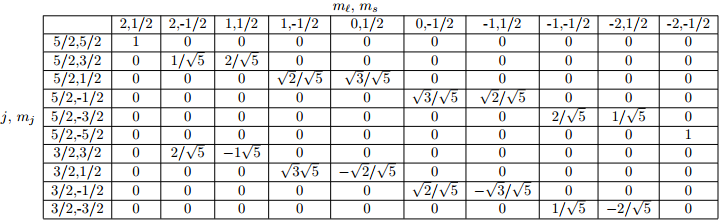
\includegraphics[width=0.7\textwidth]{figures/CG1}
			\caption{The Clebsch-Gordan coefficients for an electron with $l=2$.}
			\label{fig:CG}
		\end{figure}
		
		\item \emph{Summarize your result in terms of Clebsch-Gordan coefficients.}\newline
		
		The Clebsch-Gordan\index{Clebsch-Gordon coefficients} coefficients are the coefficients on the right hand side of $\ket{j,m}=..\ket{m_1,m_2}+...\ket{m_1,m_2}...$. These are given by
		\begin{equation}
			\begin{split}
				&\braket{m_1=2,m_2=\frac{1}{2}|j=\frac{5}{2},m=\frac{5}{2}}=1,\\
				&\braket{m_1=1,m_2=\frac{1}{2}|j=\frac{5}{2},m=\frac{3}{2}}=\sqrt{\frac{4}{5}},\\
				&\braket{m_1=2,m_2=-\frac{1}{2}|j=\frac{5}{2},m=\frac{3}{2}}=\sqrt{\frac{1}{5}},\\
				&\braket{m_1=1,m_2=\frac{1}{2}|j=\frac{3}{2},m=\frac{3}{2}}=-\sqrt{\frac{1}{5}},\\
				&\braket{m_1=2,m_2=-\frac{1}{2}|j=\frac{3}{2},m=\frac{3}{2}}=\sqrt{\frac{4}{5}}.\\
			\end{split}
		\end{equation} 
		
	\end{enumerate}
\end{example}


\chapter{Approximation methods}


\section{Perturbation theory in QM}
\label{chp:TDPT}
In the preceding chapters I have illustrated how to solve some simple quantum mechanical systems exactly. Most quantum mechanical systems, however, cannot be solved exactly, and so instead approximate methods are used. One such method is perturbation theory. In the words of Paul Dirac~\citep[p.167]{dirac} 

\begin{quote}
	“\textit{... Most quantum problems, however, cannot be solved exactly with the present resources of mathematics, as they lead to equations whose solutions cannot be expressed in finite terms with the help of the ordinary functions of analysis. For such problems one can often use a perturbation method. This consists in splitting up the Hamiltonian into two parts, one of which must be simple and the other small. The first part may then be considered as the Hamiltonian of a simplified or unperturbed system, which can be dealt with exactly, and the addition of the second will then require small corrections, of the nature of a perturbation, in the solution for the unperturbed system. The requirement that the first part shall be simple requires in practice that it shall not involve the time explicitly.}”
\end{quote} 

That is in perturbation theory one assume that the Hamiltonian of the system under consideration can be described by a known Hamiltonian plus a relatively small perturbative Hamiltonian. The method of procedure for determining the energy levels and eigenstates of the Hamiltonian depends on whether or not the energy levels of the Hamiltonian are degenerate and whether or not the perturbative Hamiltonian depends on time. In this chapter I will review how to deal with the different cases.

\subsection*{Non-degenerate, time-independent perturbation theory}
\index{TIPT, non-deg.}
Non-degenerate, time-independent perturbation theory deals with the case where the perturbative Hamiltonian is time-independent. Since the non-perturbative Hamiltonian always is considered time independent, this means that the total Hamiltonian is considered time independent in this case. The total Hamiltonian is taken to be on the form
\begin{equation}
	H=H_0+\lambda H',
	\label{ham13}
\end{equation} 
where $0\leq\lambda\leq1$ is a parameter, representing the strength of the perturbation, that is introduced for book-keeping purposes.  $H_0$ is the unperturbed Hamiltonian. It is assumed that the eigenstates and eigenvalues of the unperturbed Hamiltonian is known
\begin{equation}
	H_0\ket{n^0}=E_n^{(0)}\ket{n^0}.
\end{equation} 
Since the total Hamiltonian is time independent, separation of variables can be used to separate the Schroedinger equation into a time-dependent and time-independent equation. Since I have already solved the time-dependent one, I will focus on the time-independent one here. This will be on the form
\begin{equation}
	H\ket{n}=E_n\ket{n}.
	\label{ham12}
\end{equation} 
The perturbation changes $\ket{n^0}$ only slightly, and therefore the new eigenstate can be expanded in terms of $\ket{n^0}$. In mathematical terms; the perturbation does not change the Hilbert space, so the eigenvectors of the unperturbed Hamiltonian can be used to expand the eigenvectors of the total Hamiltonian. Since the perturbation is assumed only to change the state slightly I will describe a given eigenstate of the total Hamiltonian as the corresponding eigenstate of the unperturbed Hamiltonian plus some perturbative term
\begin{equation}
	\ket{n}=\ket{n^0}+\ket{\Delta n},
\end{equation} 
where the perturbative term can be expanded in terms of the eigenvectors of the unperturbed Hamiltonian (minus the eigenvector $\ket{n^0}$ since this is already used)
\begin{equation}
	\ket{\Delta n}=\sum_{k\neq n}^{}c_k\ket{k^0}.
\end{equation} 
Similarly the energy of a given eigenstate can be described as the energy of the corresponding eigenstate of the unperturbed Hamiltonian plus some perturbative term
\begin{equation}
	E_n=E_n^{(0)}+\Delta E_n.
\end{equation} 
The aim of perturbation theory is to determine $\Delta E_n$ and $\ket{\Delta n}$ so the eigenstates and eigenvalues of the total Hamiltonian is determined. To this end I insert the expression for $E_n$ and $\ket{n}$ into equation \eqref{ham12}. Thereby
\begin{equation}
	(H_0+\lambda H')(\ket{n^0}+\ket{\Delta n})=(E_n^{(0)}+\Delta E_n)(\ket{n^0}+\ket{\Delta n}).
	\label{eq19}
\end{equation} 
I let the first terms on the LHS and RHS\footnote{LHS=Left Hand Side, RHS=Righ Hand Side.} cancel and act from the left with the bra $\bra{n^0}$. Since $\braket{n^0|n'^0}=\delta_{n^0 n'^0}$, and $\ket{\Delta n}$ is expanded in terms of $\ket{k^0}$ where $k\neq n$, $\braket{n^0|\Delta n}=0$ and $\braket{n^0|n^0}=1$. For the third term on the LHS of equation \eqref{eq19} I use that $H_0$ is Hermitian and I can therefore let it operate to the left onto its eigenstate and obtain the eigenvalue. Since the eigenvalue is just a number the bra is allowed to operator onto the ket, but since $\braket{n^0|\Delta n}=0$ the term vanishes. On the RHS I can let the bra operate onto the kets immediately since the eigenvalues are just numbers and numbers commute with all operators. Therefore the two last terms cancel using again that $\braket{n^0|\Delta n}=0$. Thus I am left with
\begin{equation}
	\lambda\braket{n^0|H'|n}=\Delta E_n,
	\label{eq20}
\end{equation} 
where I have used that $\lambda\bra{n^0}H'\ket{n^0}+\lambda\bra{n^0}H'\ket{\Delta n}=\lambda\braket{n^0|H'|n}$. The effect of the perturbation is to shift the energy level (originally $E_n$) by an amount $\Delta E_n$ which can be determined by equation \eqref{eq20}. However, to calculate the shift in the energy the state $\ket{n}$ has to be determined. In reality it is expanded in powers of $\lambda$
\begin{equation}
	\begin{split}
		\ket{n}&=\sum_{i}\lambda^i\ket{n^i}\\
		&=\ket{n^0}+\lambda\ket{n^1}+\lambda^2\ket{n^2}+...\\
		&=\ket{n^0}+\lambda\sum_{k\neq n}^{}c_k^{(1)}\ket{k^0}+\lambda^2\sum_{k\neq n}^{}c_k^{(2)}\ket{k^0}+....
		\label{eig4}
	\end{split}
\end{equation} 
Each of the terms $\lambda^i\ket{n^i}$ are correction terms that add up to $\ket{\Delta n}$. Since the expansion of$\ket{\Delta n}$ on $\ket{k^0}$ was for a general vector that was not $n^0$ the same method applies for each of the vectors $\ket{n^i}$. 
By inserting this power series expansion into equation \eqref{eq20} the shift in energy can be written as
\begin{equation}
	\begin{split}
		\Delta E_n&=\lambda\braket{n^0|H'|n^0}+\lambda^2\braket{n^0|H'|n^1}+\lambda^3\braket{n^0|H'|n^2}+...\\
		&=\sum_{i}\lambda^i\braket{n^0|H'|n^{(i-1)}}\\
		&=\sum_{i}\lambda^iE_n^i,
	\end{split}
	\label{eq21}
\end{equation} 
where I have defined $\braket{n^0|H'|n^{(i-1)}}=E_n^i$. Therefore also the energy change can be described in terms of a power series in the energy\footnote{Note that the expansion of the energy can be written as $E_n=E_n^{(0)}+\lambda E_n^{(1)}+...$.}. By using the power series expansions of the energy and the state in equation \eqref{ham12} I find
\begin{equation}
	\begin{split}
		&\bigg(H_0+\lambda H'\bigg)\bigg(\ket{n^0}+\lambda\sum_{k\neq n}^{}c_k^{(1)}\ket{k^0}+\lambda^2\sum_{k\neq n}^{}c_k^{(2)}\ket{k^0}+...\bigg)\\&=\bigg(E_n^{(0)}+\lambda E_n^{(1)}+...\bigg)\bigg(\ket{n^0}+\lambda\sum_{k\neq n}^{}c_k^{(1)}\ket{k^0}+\lambda^2\sum_{k\neq n}^{}c_k^{(2)}\ket{k^0}+...\bigg).
	\end{split}
\end{equation} 
I then compare the terms of equal order of $\lambda$
\begin{equation}
	\begin{split}
		&\lambda^0:\qquad H_0\ket{n^0}=E_n^{(0)}\ket{n^0},\\
		&\lambda^1:\quad \sum_{k\neq n}^{}c_k^1H_0\ket{k^0}+H'\ket{n^0}=E_n^{(0)}\sum_{k\neq n}^{}c_k^{(1)}\ket{k^0}+E_n^{(1)}\ket{n^0},\\
		&\lambda^2:\quad \sum_{k\neq n}^{}c_k^{(2)}H_0\ket{k^0}+\sum_{k\neq n}^{}c_k^{(1)}H'\ket{k^0}=E_n^{(0)}\sum_{k\neq n}^{}c_k^{(2)}\ket{k^0}+E_n^{(1)}\sum_{k\neq n}^{}c_k^{(1)}\ket{k^0}+E_n^{(2)}\ket{n^0}.
	\end{split}
	\label{eq22}
\end{equation} 
The $0$'th order term just returns the unperturbed, TI Schroedinger equation - this is a good thing, as the system should to the $0$'th order not be perturbed! For the first order term I act with $\bra{n^0}$ from the left to find the first order correction to the energy
\begin{equation}
	\begin{split}
		\lambda^1:\qquad E_n^{(1)}&=\frac{\braket{n^0|H'|n^0}}{\braket{n^0|n^0}}\\
		&=\int\int\braket{n^0|x'}\braket{x'|H'|x''}\braket{x''|n^0}d^3x'd^3x''\\
		&=\int|\braket{n^0|x'}|^2\braket{x'|H'|x'}d^3x',
	\end{split}
\end{equation} 
where if the states are normalized $\braket{n^0|n^0}=1$. For the second order term I do the same from which I find
\begin{equation}
	\lambda^2:\qquad E_n^{(2)}=\sum_{k\neq n}c_k^{(1)}\frac{\braket{n^0|H'|k^0}}{\braket{n^0|n^0}}=\sum_{k\neq n}c_k^{(1)}\braket{n^0|H'|k^0},
\end{equation} 
where I have assumed the states are normalized in the above equality (i.e. that $\braket{n'|n}=\delta_{n'n}$). $c_k^1$ is determined by acting with $\bra{k'^0}$ from the left on equation \eqref{eq22}. Hereby
\begin{equation}
	\lambda^1:\qquad \braket{k'^0|H'|n^0}+c_{k'}^{(1)}E_{k'}^{(1)}=E_n^{(0)}c_{k'}^{(1)} \Rightarrow c_{k'}^{(1)}=\frac{\braket{k'^0|H'|n^0}}{E_n^{(0)}-E_{k'}^{(0)}}.
\end{equation} 
$k'$ is just a dummy index, so I let $k'\Rightarrow k$ and use the above in the second order correction to the energy. Thereby
\begin{equation}
	\lambda^2:\qquad E_n^{(2)}=\sum_{k\neq n}\frac{|\braket{k^0|H'|n^0}|^2}{E_n^{(0)}-E_k^{(0)}}.
\end{equation} 
Collecting the first and second order correction
\begin{equation}
	\Delta E_n=\sum_{i}\lambda^iE_n^i=\lambda \braket{n^0|H'|n^0}+\lambda^2\sum_{k\neq n}\frac{|\braket{k^0|H'|n^0}|^2}{E_n^{(0)}-E_k^{(0)}}+....
\end{equation} 
Likewise for the eigenstate
\begin{equation}
	\ket{n}=\sum_{i}\lambda^i\ket{n^i}=\ket{n^0}+\lambda\sum_{k\neq n}^{}\frac{\braket{k^0|H'|n^0}}{E_n^{(0)}-E_{k}^{(0)}}\ket{k^0}+....
\end{equation} 
In the end, which this is, the strength of the perturbation is set to unity (i.e. $\lambda=1$). Thereby
\begin{equation}
	\Delta E_n=\underbrace{\braket{n^0|H'|n^0}}_{\mathcal{O}(\lambda)}+\underbrace{\sum_{k\neq n}\frac{|\braket{k^0|H'|n^0}|^2}{E_n^{(0)}-E_k^{(0)}}}_{\mathcal{O}(\lambda^2)}+...,
	\label{correction energy}
\end{equation} 
\begin{equation}
	\ket{n}=\underbrace{\ket{n^0}}_{\mathcal{O}(\lambda^0)}+\underbrace{\sum_{k\neq n}^{}\frac{\braket{k^0|H'|n^0}}{E_n^{(0)}-E_{k}^{(0)}}\ket{k^0}}_{\mathcal{O}(\lambda)}+....
	\label{correction state}
\end{equation} 
Even through the $\lambda$'s are gone, one must remember where they were because they describe the order of the perturbative term! By collecting higher orders of lambda and sandwiching from the left with a bra higher order corrections to the energy and state vector can be found. However, the first corrections provides a very good approximation in most cases and so higher order terms are not needed\footnote{The expressions also gets increasingly more complicated. If the expressions were simpler perhaps they would have been incorporated. A funny side note: P. A. M. Dirac was almost religious in the belief that math describing physical phenomena should be beautiful". He would dismiss a physical theory on the basis of the mathematics being "not beautiful". This has frustrated many physicists pitching ideas to him.}\footnote{Dirac is the inventor of TDPT - this is perhaps why it is well explained!}.

\subsection*{Degenerate, time-independent perturbation theory}
\index{TIPT, deg.}
In the case of degenerate energy levels the same equations cannot be used since the denominators (in the $\lambda^2
$ and $\lambda$ term respectively) in equation \eqref{correction energy} and \eqref{correction state} blow up if $E_n^0=E_k^0$. An infinity hints that the physics are wrong, and indeed they are in this case. The error comes from the eigenstate. From equation \eqref{correction state} it is clear that the correction to a given eigenstate is taken as a perturbation with respect to a state that refers to the energy level. However, in the case of degeneracy several eigenstates can be $\ket{n^0}$. To fix this I use that a linear combination of the degenerate states is orthogonal to the non-degenerate states. I denote the set of degenerate states as $g$ and the individual degenerate eigenvectors as $\ket{m^0}$\footnote{So the different eigenvectors $\ket{m^0}$ are the elements in the set of degenerate eigenvectors; $g$.}. From these definitions I can write a degenerate version of equation \eqref{eig4} as follows
\begin{equation}
	\ket{n}=\sum_{m\in g}x_m\ket{m^0}+\lambda\sum_{k\not\in g}c_k^{(1)}\ket{k^0}+\lambda^2\sum_{k\not\in g}c_k^{(2)}\ket{k^0}+....
	\label{correction state1}
\end{equation} 
where $x_m$ is just the set of expansion coefficients amongst the degenerate eigenstates. I use the same procedure as in the non-degenerate case and so I must also represent the energy by an expansion in powers of $\lambda$. Since I have fixed the issue (the degeneracy of $\ket{n^0}$) I can use the same expansion as in the non-degenerate case
\begin{equation}
	E_n=E_n^{(0)}+\lambda E_n^{(1)}+\lambda^2E_n^{(2)}+....
\end{equation} 
By using these in the TI Schroedinger equation (equation \eqref{ham12}) alongside the definition of the Hamiltonian from equation \eqref{ham13}
\begin{equation}
	\begin{split}
		&\bigg(H_0+\lambda H'\bigg)\bigg(\sum_{m\in g}x_m\ket{m^0}+\lambda\sum_{k\not\in g}c_k^{(1)}\ket{k^0}+\lambda^2\sum_{k\not\in g}c_k^{(2)}\ket{k^0}+...\bigg)\\
		&=\bigg(E_n^{(0)}+\lambda E_n^{(1)}+\lambda^2E_n^{(2)}+...\bigg)\bigg(\sum_{m\in g}x_m\ket{m^0}+\lambda\sum_{k\not\in g}c_k^{(1)}\ket{k^0}+\lambda^2\sum_{k\not\in g}c_k^{(2)}\ket{k^0}+\dots\bigg).
	\end{split}
\end{equation} 
I compare the terms of the same order in $\lambda$
\begin{equation}
	\begin{split}
		&\lambda^0:\quad \sum_{m\in g}x_mH_0\ket{m^0}=E_n^{(0)}\sum_{m\in g}x_m\ket{m^0},\\
		&\lambda^1:\quad \sum_{m\in g}x_mH'\ket{m^0}+\sum_{k\not\in g}c_k^{(1)}E_k^{(0)}\ket{k^0}=E_n^{(0)}\sum_{k\not\in g}c_k^{(1)}\ket{k^0}+E_n^{(1)}\sum_{m\in g}x_m\ket{m^0},\\
		&\lambda^2:\quad \sum_{k\not\in g}c_k^{(1)}H'\ket{k^0}+\sum_{k\not\in g}c_k^{(2)}E_k^{(0)}\ket{k^0}
		=E_n^{(0)}\sum_{k\not\in g}c_k^{(2)}\ket{k^0}+E_n^{(1)}\sum_{k\not\in g}c_k^{(1)}\ket{k^0}+E_n^{(2)}\sum_{m\in g}x_m\ket{m^0},
	\end{split}
\end{equation} 
where $H_0\ket{m^0}=E_n^{(0)}\ket{m^0}$. By acting from the left with $\bra{m'^0}$ I find\footnote{Nothing exciting happens for the zeroth order term.}
\begin{equation}
	\lambda^1:\qquad \sum_{m\in g}x_m\bra{m'^0}H'\ket{m^0}=E_n^{(1)}x_{m'}.
\end{equation} 
This is a matrix equation on the same form as equation \eqref{matrixeig1}. Cf. Cramers rule there only exists non-trivial solutions if
\begin{equation}
	det(H'-E_n^{(1)}I)=0 \Rightarrow \{E_n^{(1)}\}, \{\ket{l}\}.
\end{equation} 
Diagonalizing the matrix $H'$\footnote{In practice the matrix to be diagonalized is the matrix containing the entire extra term, that is including $\lambda$.} results in $E_n^{(1)}$ and $x_m$.\footnote{The different sets of $x_m$ in turn results in the eigenvectors, $\ket{l}$, corresponding to the eigenvalues, $E_n^{(1)}$.} Since the number of eigenvalues match the dimensions of the matrix, there will be several, different, corrections to the degenerate energy level. This is to be understood as the degenerate energy level splitting into distinct energy levels; the perturbation splits the degenerate energy level into distinct energy levels.  
\begin{figure}[ht]
	\captionsetup{width=1\textwidth}
	\centering
	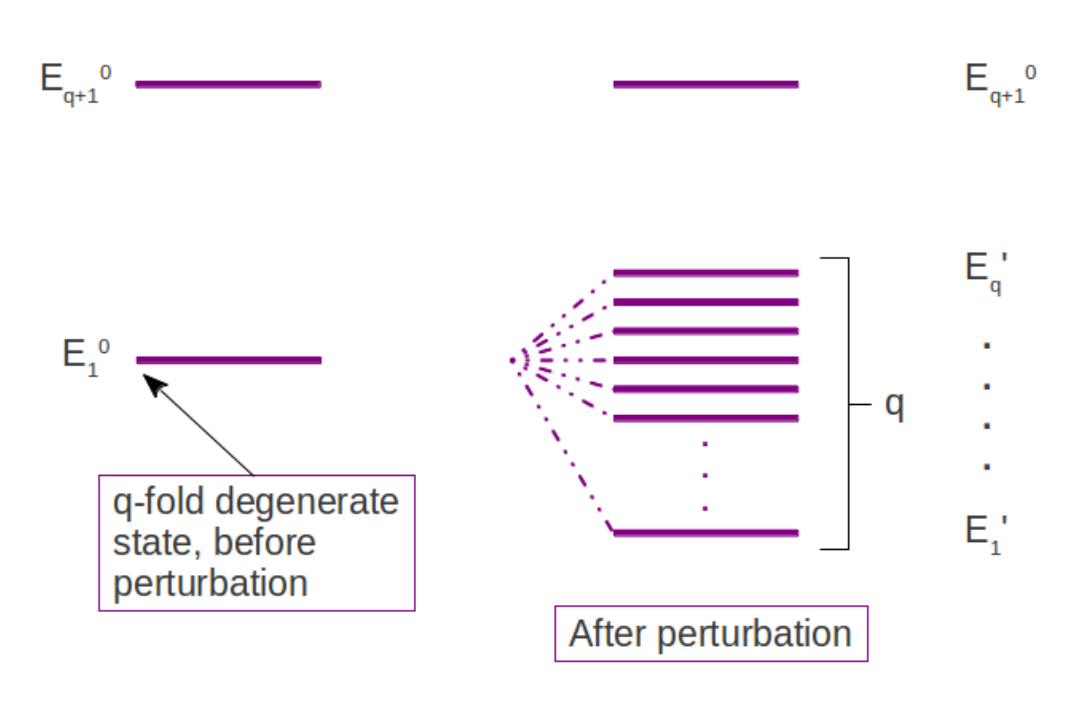
\includegraphics[width=0.6\textwidth]{figures/degpert}
	\caption{The splitting of the degenerate energy level.}
	\label{fig:degpert}
\end{figure}
Since there can be degeneracy in the energy levels when diagonalizing a matrix, the diagonalization does not guarantee a complete lifting of the degeneracy. I will however limit myself to the case where this is so. If I lift the degeneracy I can use the same formulas, with the correction that the sum is only over non-degenerate energy eigenstates, as in the non-degenerate case to determine the higher order correction. Thereby I in the end find
Collecting the first and second order correction
\begin{equation}
	\Delta E_n=\underbrace{E_n^{(1)}}_{\mathcal{O}(\lambda)}+\underbrace{\sum_{k\notin g}\frac{|\braket{k^0|H'|n^0}|^2}{E_n^{(0)}-E_k^{(0)}}+}_{\mathcal{O}(\lambda^2)}..., 
	\label{correction energy2}
\end{equation} 
where $E_n^{(1)}$ are the eigenvalues of the degenerate perturbation matrix and can take different values. The second order correction is the same for each of these different values of $E_n^{(1)}$. For the eigenstate
\begin{equation}
	\ket{n}=\underbrace{\ket{l}}_{\mathcal{O}(\lambda^0)}+\underbrace{\sum_{k \notin g}\frac{\bra{k^0}\mathcal{H}'\ket{l}}{E_l^{0}-E_k^{0}}\ket{k^{0}}}_{\mathcal{O(\lambda)}}+...,
	\label{correction state2}
\end{equation} 
where $\ket{l}$ are any of the eigenvectors obtained from diagonalizing the degenerate sub-matrix of the perturbative Hamiltonian. By comparison between equation \eqref{correction energy} versus \eqref{correction energy2} and equation \eqref{correction state} versus \eqref{correction state2} it is clear that the corrections in degenerate perturbation theory are reminiscent of the ones from non-degenerate perturbation theory. The procedure in degenerate perturbation theory is to find the basis in which the sub-matrix of the perturbative Hamiltonian that is degenerate is diagonal. If this basis lifts the degeneracy completely the non-degenerate perturbation theory can be applied to the eigenstates and eigenvalues of the degenerate perturbation matrix.  

\subsection*{Time-dependent perturbation theory}
\index{TDPT}
Time-dependent perturbation theory is an approximate method for solving the Schroedinger equation in the case where $\frac{\partial H}{\partial t}\neq0$ - that is in the case where separation of variables does not apply. The Hamiltonian is taken to consist of two additive parts; one simple part ($H_0$) for which the solution is known and one smaller part ($H'$). The simple part must contain any time dependency in order to be simple($\frac{\partial H_0}{\partial t}=0$), so the time dependency of the Hamiltonian must lie in the small part, i.e. $H'=H'(t)$. The Hamiltonian is therefore given by
\begin{equation}
	H=H_0+H'(t).
\end{equation} 
The system is taken to be in an eigenstate of $H_0$ at $t=0s$. In some finite interval of time the system is then perturbed, in this case the system is a nucleus, and the perturbation is scattering with the WIMP. After the perturbation, the system is again characterized by the simple Hamiltonian, and the system is possibly in the same or a different eigenstate of the simple Hamiltonian. The scenario is shown in figure \ref{fig:jj}.
\begin{figure}[ht]
	\captionsetup{width=1\textwidth}
	\centering
	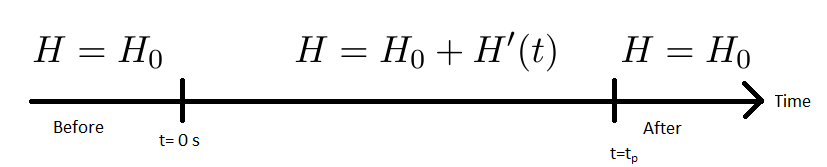
\includegraphics[width=1\textwidth]{figures/tipertub}
	\caption{The development of the Hamiltonian as a function of time.}
	\label{fig:jj}
\end{figure}
While the perturbation is turned on ($0\leq t\leq t_p$) the system is described by the Schroedinger equation on the form
\begin{equation}
	i\hbar\frac{\partial \ket{\alpha}}{\partial t}=(H_0+H'(t))\ket{\alpha},
	\label{sch4}
\end{equation} 
where $\ket{\alpha}$ is the state-vector. Equation \eqref{sch4} is solved by assuming that the eigenvectors and eigenvalues of the unperturbed system is known. Since the unperturbed Hamiltonian is time independent the Schroedinger equation can in this case be solved via separation of variables. The time-dependent Schroedinger equation is trivially solved while the time-independent Schroedinger equation is given by
\begin{equation}
	H_0\ket{n_0}=E_{n_0}\ket{n_0},
\end{equation}  
where $E_{n_0}$ and $\{\ket{n_0}\}$ is taken to be known. Since the eigenvectors of $H_0$ make up a complete set, spanning the desired vector space, they are used to develop the state-vector of the system
\begin{equation}
	\ket{\alpha}=\sum_{n_0}^{}c_{n_0}(t)e^{-\frac{iE_{n_0}}{\hbar}t}\ket{n_0},
	\label{expansion2}
\end{equation}  
where, compared to the case where the Hamiltonian is time-independent, the coefficients of the expansion are now time-dependent. The probability of the system ending up in a given state is given by the squared magnitude of the coefficients $c_{n_0}(t)$. To solve equation \eqref{sch4} equation \eqref{expansion2} is inserted
\begin{equation}
	\begin{split}
		&i\hbar\sum_{n_0}^{}\frac{\partial c_{n_0}(t)}{\partial t}e^{-\frac{iE_{n_0}}{\hbar}t}\ket{n_0}-i\hbar\sum_{n_0}^{}c_{n_0}(t)\frac{iE_{n_0}}{\hbar}e^{-\frac{iE_{n_0}}{\hbar}t}\ket{n_0}=\sum_{n_0}^{}(H_0+H'(t))\ket{n_0}c_{n_0}(t)e^{-\frac{iE_{n_0}}{\hbar}t}.
	\end{split}
	\label{sch5}
\end{equation} 
Equation \eqref{sch5} is multiplied from the left with a eigenbra of $H_0$; $\bra{m_{0}}$
\begin{equation}
	\begin{split}
		&	i\hbar\sum_{n_0}^{}\frac{\partial c_{n_0}(t)}{\partial t}e^{-\frac{iE_{n_0}}{\hbar}t}\braket{m_0|n_0}+\sum_{n_0}^{}c_{n_0}(t)E_{n_0}e^{-\frac{iE_{n_0}}{\hbar}t}\braket{m_0|n_0}\\
		&=\sum_{n_0}^{}\bra{m_0}(H_0+H'(t))\ket{n_0}c_{n_0}(t)e^{-\frac{iE_{n_0}}{\hbar}t}.
	\end{split}
	\label{sch6}
\end{equation} 
By using $\braket{m_0|n_0}=\delta_{m_0n_0}$ the sums on the left hand side vanishes. Furthermore $H_0$ operating to the right on $\ket{n_0}$  results in $E_{n_0}\ket{n_0}$ since $\ket{n_0}$ is an eigenstate of $H_0$. Since $E_{n_0}$ is just a number, it can be taken outside the inner product, and again the orthogonality property can be used to kill the sum. In the end
\begin{equation}
	\begin{split}
		&	i\hbar\frac{\partial c_{m_0}(t)}{\partial t}e^{-\frac{iE_{m_0}}{\hbar}t}+c_{m_0}(t)E_{m_0}e^{-\frac{iE_{m_0}}{\hbar}t}=c_{m_0}(t)E_{m_0}e^{-\frac{iE_{m_0}}{\hbar}t}+\sum_{n_0}^{}\bra{m_0}H'(t)\ket{n_0}c_{n_0}(t)e^{-\frac{iE_{n_0}}{\hbar}t}.
	\end{split}
	\label{sch7}
\end{equation} 
Two of the terms cancel out. By moving the exponential from the left hand side (LHS) to the right hand side (RHS)
\begin{equation}
	i\hbar\frac{\partial c_{m_0}(t)}{\partial t}=\sum_{n_0}^{}\bra{m_0}H'(t)\ket{n_0}c_{n_0}(t)e^{i\omega_{m_0n_0}t},
	\label{sch8}
\end{equation} 
where $\omega_{m_0n_0}=\frac{E_{m_0}-E_{n_0}}{\hbar}$. A general solution to equation \eqref{sch8} is difficult, but in the case where $H'\ll H_0$ perturbation theory is applicable, and an approximative solution can be found. A dimensionless, continuous, real parameter, $\lambda \in[0,1]$, representing the strength of the perturbation, is defined by
\begin{equation}
	H'(t)\Rightarrow\lambda H'(t).
\end{equation} 
$\lambda$ is "dialed" from $0$ to $1$ in a smooth, continuous way as the state of the system goes from $\ket{n_0}$ to $\ket{\alpha}$. The parameter makes sure that there is a continuous transition between the two states of the system. Next up the expansion coefficients, $c_{m_0}(t)$ and $c_{n_0}(t)$, are expanded in powers of $\lambda$
\begin{equation}
	c_{m_0}(t)=c^{(0)}_{m_0}(t)+\lambda c^{(1)}_{m_0}(t)+\lambda^2c^{(2)}_{m_0}(t)+...,
	\label{power1}
\end{equation} 
\begin{equation}
	c_{n_0}(t)=c^{(0)}_{n_0}(t)+\lambda c^{(1)}_{n_0}(t)+\lambda^2c^{(2)}_{n_0}(t)+...,
	\label{power2}
\end{equation} 
where the superscript "${(0)}$"denotes unperturbed quantities, and higher numbers identify corrections of higher orders. If the method is to be of practical interest, a good approximation must be obtained by taking only one or two terms into account. Equation \eqref{power1} and \eqref{power2} is inserted in equation \eqref{sch8}
\begin{equation}
	\begin{split}
		&i\hbar\bigg(\frac{\partial c^0_{m_0}(t)}{\partial t}+\lambda\frac{\partial c^1_{m_0}(t)}{\partial t}+\lambda^2\frac{\partial c^2_{m_0}(t)}{\partial t}+...\bigg)\\
		& =\sum_{n_0}^{}(c^0_{n_0}(t)+\lambda c^1_{n_0}(t)+\lambda^2c^2_{n_0}(t)+...)\lambda e^{i\omega_{m_0n_0}t}\bra{m_0}H'(t)\ket{n_0},
	\end{split}
	\label{sch9}
\end{equation} 
\normalsize
where the $\lambda$ outside the parenthesis on the right hand side stems from $H'(t)$. Comparing powers of $\lambda$
\begin{equation}
	\begin{split}
		&\lambda^0:\qquad \qquad \qquad \quad i\hbar\frac{\partial c^{(0)}_{m_0}(t)}{\partial t}=0\Rightarrow c^{(0)}_{m_0}(t)=const,\\
		&\lambda^1:\qquad i\hbar\frac{\partial c^{(1)}_{m_0}(t)}{\partial t}=\sum_{n_0}^{}c^{(0)}_{n_0}(t) e^{i\omega_{m_0n_0}t}\bra{m_0}H'(t)\ket{n_0},\\
		&\lambda^2:\qquad i\hbar\frac{\partial c^{(2)}_{m_0}(t)}{\partial t}=\sum_{n_0}^{}c^{(1)}_{n_0}(t) e^{i\omega_{m_0n_0}t}\bra{m_0}H'(t)\ket{n_0}.\\
	\end{split}	
	\label{c2}
\end{equation} 
It is clear that the coefficients on the LHS and RHS not are of the same power - there is a recursion relation. The coefficient $c^{(1)}_{m_0}(t)$ describes the process in which a single photon is absorbed or emitted by an atom. Higher order coefficients correspond to processes incorporating more photons (eg. $c^{(2)}_{m_0}(t)$ corresponds to a two photon process). Because the relation between the coefficients is recursive the lower order coefficients must be determined in order to determine a higher order coefficient. Therefore, to get started, $c^0_{m_0}(t)$ is determined from an analysis of the initial conditions. The system is taken to be in an eigenstate of $H_0$ denoted by $\ket{a_0}$ at $t=0$ - where $i$ is just a random label. Since the system at $t=0$ is in an eigenstate of $H_0$, the only non-zero coefficient must be the one corresponding to $\ket{a_0}$,  i.e.
\begin{equation}
	t=0: \qquad c_{a_0}=1 \quad \wedge \quad c_{i\neq a_0}=0.
	\label{initial condition}
\end{equation} 
The coefficients of 0'th order, $c^{(0)}_{n_0}(t)$, refers to the initial, unperturbed state. The only coefficient differing from 0 is $c^{(0)}_{a_0}(t)=1$. Thereby the sum in the expression for the first order coefficient can be removed and, by denoting the final state $\bra{b_0}$
\begin{equation}
	i\hbar\frac{\partial c^{(1)}_{b_0}(t)}{\partial t}=e^{i\omega_{b_0a_0}t}\bra{b_0}H'(t)\ket{a_0}.
\end{equation} 
Moving $i\hbar$ to the RHS, and integrating
\begin{equation}
	c^{(1)}_{b_0}(t)=\frac{1}{i\hbar}\int_{0}^{t}\bra{b_0}H'(t')\ket{a_0}e^{i\omega_{b_0a_0}t'}dt',
	\label{coef}
\end{equation} 
where often $t_p$ is denoted by $t$. Using equation \eqref{coef} in equation \eqref{c2}
\begin{equation}
	\begin{split}
		c^{(2)}_{b_0}(t)&=\frac{1}{i\hbar}\sum_{n_0}^{}\int_{0}^{t}c^{(1)}_{n_0}(t'') e^{i\omega_{b_0n_0}t''}\bra{b_0}H'(t'')\ket{n_0}dt'
		\\
		&=-\frac{1}{\hbar^2}\sum_{n_0}\int_{0}^{t}\bra{b_0}H'(t'')\ket{n_0}e^{i\omega_{b_0n_0}t''}\int_{0}^{t''}\bra{n_0}H'(t')\ket{a_0}e^{i\omega_{n_0a_0}t'}dt'dt''.
		\\
	\end{split}
	\label{second order}
\end{equation} 
The transition probability, via a general process, is given by
\begin{equation}
	\mbox{Transition probability from $\ket{a_0}$ to $\ket{b_0}$}=P_{a_0\Rightarrow b_0}=|c^{(1)}_{b_0}(t)+c^{(2)}_{b_0}(t)+...|^2.
	\label{trans prob}
\end{equation} 
The transition probability for an $i$-photon process, eg. single photon or tw-photon, is given by
\begin{equation}
	P^{(i)}_{a_0\Rightarrow b_0}=|c^{(i)}_{b_0}(t)|^2.
\end{equation} 
The transition probability depends on the nature of $H'(t)$. Calculating the transition probability concludes time-dependent perturbation theory(TDPT). Since the system state before perturbation is known, what is of interest is what happens to the system during the perturbation - whether or not the system jumps into another state. This probability depends on the size of the perturbation, and if the perturbation is small, the probability can be calculated from equation \eqref{trans prob}. 

\section{The WKB approximation}
The WKB method is a technique for obtaining approximate solutions to the time-independent Schroedinger equation ($\frac{\partial H}{\partial t}=0$) in one dimension\footnote{The same technique can be applied to many other differential equations.}. It is particularly useful in calculating bound state energies and tunneling rates through a potential barrier, and is for this reason used in astrophysics when dealing with the tunneling probability relevant for fusion processes. \newline
I begin with the one-dimensional Schroedinger equation in the position basis
\begin{equation}
	-\frac{\hbar^2}{2M}\frac{\partial^2\psi(x)}{\partial x^2}+V(x)\psi(x)=E\psi(x).
	\label{sch10}
\end{equation} 
This equation can be rewritten as
\begin{equation}
	\frac{\partial^2\psi(x)}{\partial x^2}=-\frac{2M(E-V(x))}{\hbar^2}\psi(x)=-\frac{p^2}{\hbar^2}\psi(x),
	\label{sch11}
\end{equation} 
where $p=\sqrt{2M(E-V(x))}$ is the classical momentum of a particle moving in a one-dimensional potential~\citep[p.346]{Griffiths}, $V(x),$ with energy $E$, provided that $E\geq V(x)$ for all $x$. where the wave function in general is a complex number, and therefore can be written as
\begin{equation}
	\psi(x)=A(x)e^{i\phi(x)},
\end{equation} 
where $\phi(x)$ is the phase of the complex number. By this notation equation \eqref{sch11} becomes
\begin{equation}
	\begin{split}
		&\bigg(\frac{\partial^2A(x)}{\partial x^2}+2i\frac{\partial A(x)}{\partial x}\frac{\partial \phi(x)}{\partial x}+iA(x)\frac{\partial^2\psi(x)}{\partial x^2}-A(x)\bigg(\frac{\partial \phi(x)}{\partial x}\bigg)^2\bigg)e^{i\phi(x)}\\
		&=-\frac{p^2}{\hbar^2}A(x)e^{i\phi(x)}.
	\end{split}
	\label{sch12}
\end{equation} 
This is equivalent to two real equations, one for the real part and one for the imaginary part. For the real part
\begin{equation}
	\frac{\partial^2A(x)}{\partial x^2}=A(x)\bigg(\bigg(\frac{\partial\phi(x)}{\partial x}\bigg)^2-\frac{p^2}{\hbar^2}\bigg).
	\label{sch13}
\end{equation} 
For the imaginary part
\begin{equation}
	\frac{\partial}{\partial x}\bigg(A(x)^2\frac{\partial \phi(x)}{\partial x}\bigg)=0.
	\label{sch14}
\end{equation} 
Equation \eqref{sch13} and \eqref{sch14} are equivalent to the time-independent Schroedinger equation. Equation \eqref{sch14} is solved by integration. Denoting the integration constant $C^2$, I find
\begin{equation}
	A(x)=\frac{C}{\sqrt{\frac{\partial \phi(x)}{\partial x}}},
	\label{A(x)}
\end{equation} 
where $C$ is a real constant. Equation \eqref{sch13} cannot be solved in general, so an approximation is introduced; \emph{it is assumed that the amplitude varies slowly, such that $\frac{\partial^2A(x)}{\partial x^2}\approx0$}, and $\frac{\frac{\partial^2A(x)}{\partial x^2}}{A(x)}\approx0$. Thus, from equation \eqref{sch13} I find
\begin{equation}
	\frac{\partial\phi(x)}{\partial x}\approx\pm\frac{p}{\hbar},
	\label{sch15}
\end{equation} 
which is solved by integration such that
\begin{equation}
	\phi(x)\approx\pm\frac{1}{\hbar}\int p(x)dx.
	\label{phi(x)}
\end{equation} 
Any constants from this integral may be absorbed into $C$, and $C$ may therefore be complex. Thus, I find the approximate solution
\begin{equation}
	\psi(x)\simeq\frac{C}{\sqrt{p(x)}}e^{\pm\frac{i}{\hbar}\int p(x)dx}.
	\label{sol}
\end{equation} 
The general, approximate solution will be a linear combination of the plus and minus solution. From equation \eqref{sol} it is clear that the probability of finding the particle at position $x$ is given by
\begin{equation}
	|\psi(x)|^2\simeq\frac{|C|^2}{p(x)}.
	\label{prob1}
\end{equation} 
Equation \eqref{prob1} reveals that the probability of finding the particle at position $x$ is inversely proportional to the classical momentum, and thereby the particle's velocity at that point. The makes sense since if the particle has a large velocity at one point, it will not spend as much time there, and the probability of finding the particle there will be smaller.

\begin{example}
	\index{TIPT, deg.}
	\index{TIPT, SHO}
	\emph{A simple harmonic oscillator (in one dimension) is subjected to a perturbation}
	\begin{equation}
		H'=bx,
	\end{equation}  
	\emph{where $b$ is a real constant.}\newline
	
	\begin{enumerate}
		\item \emph{Calculate the energy shift of the ground state to the lowest non-vanishing order.}\newline
		
		Since the energy levels of $H_0$ (the SHO) is \emph{not} degenerate, and the perturbation does not depend on time, I use TIPT in the non-degenerate version. I use equation \eqref{correction energy} and evaluate from the "bottom". The first order correction to the energy
		\begin{equation}
			\Delta E^{(1)}_0=b\braket{0^0|x|0^0}=b\int_{-\infty}^{\infty}|\psi_0(x)|^2xdx=0,
		\end{equation} 
		where I used that $\psi_n(x)=N_nH_n\big(\sqrt{\frac{\omega M}{\hbar}}x\big)e^{\frac{-\omega M x^2}{2\hbar}}$. The second order correction to the energy
		\begin{equation}
			\Delta E_0^{(2)}=b^2\sum_{k\neq 0}\frac{|\braket{k^0|x^2|0^0}|^2}{E_0^0-E_k^0}.
		\end{equation} 
		In this case it is not so straight forward since there is an infinite number of energy levels. However, by using that $\braket{n'|x|n}=\sqrt{\frac{\hbar}{2M\omega}}(\sqrt{n}\delta_{n',n-1}+\sqrt{n+1}\delta_{n',n+1})$ I take
		\begin{equation}
			\braket{k^0|x|0}=\sqrt{\frac{\hbar}{2M\omega}}(\sqrt{n}\delta_{k,0-1}+\sqrt{0+1}\delta_{k,0+1})=\sqrt{\frac{\hbar}{2M\omega}}\delta_{k,1}.
		\end{equation} 
		By using this the second order correction can be found to be
		\begin{equation}
			\Delta E_0^{(2)}=b^2\sum_{k\neq 0}\frac{|\braket{1^0|x^2|0^0}|^2}{E_0^0-E_1^0}=-\frac{b^2}{2M\omega^2},
		\end{equation} 
		where I used that $\Delta E^0=\hbar\omega=-(E_0^0-E_1^0)$. So, the energy shift to the lowest non-vanishing order (second) is given by
		\begin{equation}
			\begin{split}
				\Delta E_0&= \braket{0^0|H'|0^0}+\sum_{k\neq 0}\frac{|\braket{k^0|H'|0^0}|^2}{E_0^0-E_k^0}+...\\&=-\frac{b^2}{2M\omega^2}+....
			\end{split}
		\end{equation} 
		
		\item \emph{Solve this problem exactly and compare with your previous result.}\newline
		
		The TISE\footnote{TI= Time Independent, SE=Schroedinger Equation.} in this case is given by
		\begin{equation}
			-\frac{\hbar^2}{2M}\frac{\partial^2 \braket{x|\alpha}}{\partial x^2}+\frac{1}{2}M\omega^2x^2\braket{x|\alpha}+bx\braket{x|\alpha}=E\braket{x|\alpha}.
		\end{equation} 
		This is a second order, non-homogeneous, non-linear, partial differential equation, and as such not an easy equation to solve\footnote{If I were to solve it I would use a generalized power series approach.}. Therefore I search for a change of variables so that the equation takes a familiar form - preferably the form of the simple harmonic oscillator! Since we have a terms with $x^2$ and one with $x$ it looks factorisable. Indeed I find 
		\begin{equation}
			\frac{1}{2}M\omega^2x^2+bx=\frac{1}{2}M\omega^2\bigg(x+\frac{b}{M\omega^2}\bigg)^2-\bigg(\frac{b}{M\omega^2}\bigg)^2.
		\end{equation} 
		Inspired by this I defined $x'=x+\frac{b}{M\omega^2}$ as a new variable. Since the derivative of $x'$ with respect to $x$ is $1$ I can write the TISE in the new variable as
		\begin{equation}
			-\frac{\hbar^2}{2M}\frac{\partial^2 \braket{x|\alpha}}{\partial x'^2}+\frac{1}{2}M\omega^2\bigg(x'^2-\bigg(\frac{b}{M\omega^2}\bigg)^2\bigg)\braket{x|\alpha}=E\braket{x|\alpha},
		\end{equation} 
		which can be rewritten as
		\begin{equation}
			-\frac{\hbar^2}{2M}\frac{\partial^2 \braket{x|\alpha}}{\partial x'^2}+\frac{1}{2}M\omega^2x'^2\braket{x|\alpha}=\bigg(E+\frac{b^2}{2M\omega^2}\bigg)\braket{x|\alpha}.
		\end{equation} 
		This is the same form as the simple harmonic oscillator with the new eigenvalue
		\begin{equation}
			E'=E+\frac{b^2}{2M\omega^2}.
		\end{equation} 
		In comparison with before
		\begin{equation}
			\Delta E_0=E-E'=-\frac{b^2}{2M\omega^2},
		\end{equation} 
		which is exactly the same result as obtained from TI perturbation theory.	
	\end{enumerate}
\end{example}


\begin{example}
	\index{TIPT, SHO}
	\emph{Consider the Hamiltonian}
	\begin{equation}
		H_0=\frac{p_x^2}{2M}+\frac{1}{2}M\omega^2x^2.
	\end{equation} 
	\emph{This Hamiltonian is subjected to a perturbation on the form}
	\begin{equation}
		H'=\frac{1}{2}\varepsilon M\omega^2 x^2.
	\end{equation} 
	\emph{What is the correction to the GS energy to second order?}\newline
	
	Since the Harmonic oscillator (in 1D) is not degenerate I will use equation \eqref{correction energy}
	\begin{equation}
		\Delta E_0=\braket{0^0|H'|0^0}+\sum_{k\neq n}\frac{|\braket{k^0|H'|0^0}|^2}{E_0^{(0)}-E_k^{(0)}}+....
	\end{equation} 
	The first order correction
	\begin{equation}
		\begin{split}
			\Delta E_0^{(1)}&=\braket{0^0|H'|0^0}\\
			&=\frac{1}{2}\varepsilon M\omega^2\braket{0^0|x^2|0^0}\\
			&=\frac{1}{2}\varepsilon M\omega^2\frac{\hbar}{2M\omega}\braket{0^0|(a^\dagger+a)^2|0^0}\\
			&=\frac{\varepsilon\hbar\omega}{4}\bigg(\braket{0^0|a^\dagger a|0^0}+\braket{0^0|a^\dagger a^\dagger|0^0}+\braket{0^0|aa^\dagger|0^0}+\braket{0^0|aa|0^0}\bigg)\\
			&=\frac{\varepsilon\hbar\omega}{4}\braket{0^0|aa^\dagger|0^0}=\frac{\varepsilon\hbar\omega}{4}.
		\end{split}
	\end{equation} 
	The second order correction
	\begin{equation}
		\Delta E_0^{(2)}=\sum_{k\neq n}\frac{|\braket{k^0|H'|0^0}|^2}{E_0^{(0)}-E_k^{(0)}}.
	\end{equation} 
	To evaluate this the matrix elements need to be evaluated. In analog with the first order correction
	\begin{equation}
		\begin{split}
			\braket{k^0|H'|0^0}&=\frac{\varepsilon\hbar\omega}{4}\bigg(\braket{k^0|a^\dagger a|0^0}+\braket{k^0|a^\dagger a^\dagger|0^0}+\braket{k^0|aa^\dagger|0^0}+\braket{k^0|aa|0^0}\bigg)\\
			&=\frac{\varepsilon\hbar\omega}{4}\bigg(\braket{k^0|a^\dagger a^\dagger|0^0}\delta_{k,2}+\braket{k^0|aa^\dagger|0^0}\delta_{k,0}\bigg)\\
			&=\frac{\varepsilon\hbar\omega}{4}\bigg(\sqrt{2}\delta_{k,2}+\delta_{k,0}\bigg).\\
		\end{split}
		\label{shit}
	\end{equation} 
	Since the sum is only over $k\neq n$ the $k=0$ is not included in the second order correction
	\begin{equation}
		\Delta E_0^{(2)}=\bigg(\frac{\sqrt{2}\varepsilon\hbar\omega}{4}\bigg)^2\frac{1}{\frac{1}{2}\hbar\omega-\frac{5}{2}\hbar\omega}=-\frac{\varepsilon^2\hbar\omega}{16}.
	\end{equation} 
\end{example}

\begin{example}
	\index{TIPT, non-deg.}
	\index{TIPT, deg.}
	\index{TIPT, free particle in a box}
	\emph{Consider a particle in a two-dimensional potential}
	\begin{equation}
		V_0=\begin{cases} 0 &\mbox{for} \quad 0\leq x\leq L, 0\leq y \leq L \\ 
			\infty & \mbox{for} \quad \mbox{Else}  
		\end{cases}. 
	\end{equation} 
	\begin{enumerate}
		\item \emph{Find the eigenfunctions for the ground state and the first excited state.}\newline
		
		This is identical to the free particle in a box in two dimensions. Taking only the TI part of $\braket{x|\alpha}=\psi(x,y,z,t)_{n_xn_yn_z}=Bsin\big(\frac{n_x\pi}{L}x\big)sin\big(\frac{n_y\pi}{L}y\big)sin\big(\frac{n_z\pi}{L}z\big)e^{-\frac{iE_{n_xn_yn_z}}{\hbar}t}$ I find
		\begin{equation}
			\braket{\vec{x}|n}=\psi(x,y)_{n_x,n_y}=\frac{2}{L}sin\bigg(\frac{n_x\pi}{L}x\bigg)sin\bigg(\frac{n_y\pi}{L}y\bigg),
		\end{equation} 
		from which
		\begin{equation}
			\begin{split}
				\psi(x,y)_{1,1}&=\frac{2}{L}sin\bigg(\frac{\pi}{L}x\bigg)sin\bigg(\frac{\pi}{L}y\bigg),\\
				\psi(x,y)_{2,1}&=\frac{2}{L}sin\bigg(\frac{2\pi}{L}x\bigg)sin\bigg(\frac{\pi}{L}y\bigg),\\
				\psi(x,y)_{1,2}&=\frac{2}{L}sin\bigg(\frac{\pi}{L}x\bigg)sin\bigg(\frac{2\pi}{L}y\bigg).\\
			\end{split}
			\label{fe}
		\end{equation} 
		
		\item \emph{Now a perturbative term is added. The perturbative terms is given by}
		\begin{equation}
			H'=\begin{cases} \lambda xy &\mbox{for} \quad 0\leq x\leq L, 0\leq y \leq L \\ 
				0 & \mbox{for} \quad \mbox{Else}  \end{cases} .
		\end{equation} 
		\emph{Obtain the zeroth order energy eigenfunctions and the first order energy shifts for the ground state and the first excited state.}\newline
		
		The GS is non-degenerate so non-degenerate perturbation theory can be used here. The first excited states are degenerate so here degenerate perturbation theory must be used (the perturbative Hamiltonian does not depend on time so TDPT is not used here).\newline 
		For the GS the zeroth order energy eigenfunction is given by equation \eqref{fe}. The first order shift to the energy is given by
		\begin{equation}
			\begin{split}
				\Delta E_{1,1}^{(1)}&= \braket{1^0|H'|1^0}\\
				&=\frac{4\lambda}{L^2}\int_{0}^{L}\int_{0}^{L}sin\bigg(\frac{\pi}{L}x\bigg)^2sin\bigg(\frac{\pi}{L}y\bigg)^2xydxdy\\
				&=\frac{L^2\lambda}{4}.
			\end{split}
			\label{FPE1}
		\end{equation} 
		For the first excited state there is degeneracy, and so degenerate perturbation theory will be used instead of non-degenerate perturbation theory. I construct the matrix $\braket{n'|H'|n}$ where $n,n'=2,1;1,2$\footnote{That is a matrix of the degenerate eigenfunctions!}. That is
		\begin{equation}
			\begin{split}
				H'&\doteq\begin{bmatrix}
					\braket{1,2|H'|1,2} & \braket{1,2|H'|2,1}\\
					\braket{2,1|H'|1,2} & \braket{2,1|H'|2,1}\\
				\end{bmatrix}\\
				&=\begin{bmatrix}
					A& B\\
					C& D\\
				\end{bmatrix}\\
				&=\frac{\lambda L^2}{4}\begin{bmatrix}
					1& \frac{1024}{81\pi^4}\\
					\frac{1024}{81\pi^4} & 1\\
				\end{bmatrix},
			\end{split}
		\end{equation} 
		where
		\begin{equation}
			\begin{split}
				&A\equiv \frac{4\lambda}{L^2}\int_{0}^{L}\int_{0}^{L} sin(\frac{\pi}{L}x)^2sin(\frac{2\pi}{L}y)^2dxdy,\\
				&B\equiv \frac{4\lambda}{L^2}\int_{0}^{L}\int_{0}^{L} sin(\frac{\pi}{L}x)sin(\frac{2\pi}{L}y)sin(\frac{2\pi}{L}x)sin(\frac{\pi}{L}y)dxdy,\\
				&C\equiv \frac{4\lambda}{L^2}\int_{0}^{L}\int_{0}^{L} sin(\frac{\pi}{L}x)sin(\frac{2\pi}{L}y)sin(\frac{2\pi}{L}x)sin(\frac{\pi}{L}y)dxdy, \\
				&D\equiv \frac{4\lambda}{L^2}\int_{0}^{L}\int_{0}^{L} sin(\frac{2\pi}{L}x)^2sin(\frac{\pi}{L}y)^2dxdy.\\		
			\end{split}
		\end{equation}
		The eigenvalues of $H'$ are the first order corrections to the energy. That is
		\begin{equation}
			\Delta E_{2,1}^{(1)}=\frac{\lambda^2L^2}{324\pi^4}(81\pi^4\pm 1024).
			\label{FPE2}
		\end{equation} 
		As is apparent from the above; the energy level of the first excited state is, to first order, split into two distinct energy states. Hence the degeneracy is lifted! \newline
		The eigenvectors of $H'$ corresponds to the zeroth order energy eigenvectors. Denoting the two energy levels the first excited energy level has split into by $E_{2,i}$ where $i=1,2$, the corresponding eigenvectors can be found to be
		\begin{equation}
			\ket{E_{2,1}}=\frac{1}{\sqrt{2}}(\ket{1,2}-\ket{2,1}),
		\end{equation} 
		\begin{equation}
			\ket{E_{2,2}}=\frac{1}{\sqrt{2}}(\ket{1,2}+\ket{2,1}).
		\end{equation} 
		
	\end{enumerate}
\end{example}

\begin{example}
	\index{TIPT, free particle in a box}
	\emph{Consider a spin-less particle in a two-dimensional infinite square well}
	\begin{equation}
		V_0=\begin{cases} 0 &\mbox{for} \quad 0\leq x\leq a, 0\leq y \leq a \\ 
			\infty & \mbox{for} \quad \mbox{Else}  \end{cases}. 
	\end{equation} 
	
	\begin{enumerate}
		\item \emph{What are the energy eigenvalues for the three lowest states? Is there any degeneracy?}\newline
		
		Inside the box the particle is treated as a free particle in two dimensions. The energy is just the sum of two free particles in a 1D box
		\begin{equation}
			E_{n_x,n_y}^{(0)}=\frac{\hbar^2\pi^2}{2ML^2}(n_x^2+n_y^2),
		\end{equation} 
		where $n_i=1,2,3...$. Note that $n_i=0$ is\emph{not} a possibility since this value would make the wave-function, which is a product of the two wave-function of a 1D free particle in a box and $\psi\propto sin(n_x)sin(n_y)$, zero. Therefore the GS is given by
		\begin{equation}
			E_{1,1}^{(0)}=\frac{\hbar^2\pi^2}{ML^2}.
		\end{equation} 
		There is no degeneracy here. The following energy states
		\begin{equation}
			E_{2,1}^{(0)}=E_{1,2}^{(0)}=\frac{5\hbar^2\pi^2}{2ML^2},
		\end{equation} 
		where there is two-fold degeneracy. \newline
		
		\item \emph{Now a perturbative potential is added}
		\begin{equation}
			H'=\lambda xy.
		\end{equation} 
		\begin{enumerate}
			\item \emph{Is the energy shift due to the perturbation linear or quadratic in $\lambda$ for each of the three states?}\newline
			
			Cf. equation \eqref{FPE1} and \eqref{FPE2} $\Delta E_{1,1}^{(1)}\propto\lambda$ and $\Delta E_{2,1}^{(1)}\propto\lambda^2$.
			
			\item \emph{Draw an energy diagram representing before and after the perturbation.}\newline
			\begin{figure}[ht]
				\captionsetup{width=1\textwidth}
				\centering
				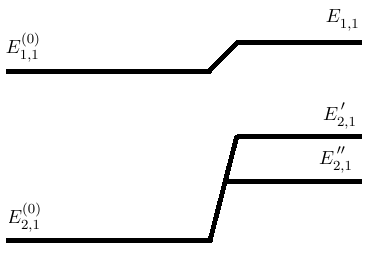
\includegraphics[width=0.4\textwidth]{figures/perturb}
				\caption{}
			\end{figure}
			
		\end{enumerate}
		
	\end{enumerate}
\end{example}


\begin{example}
	\index{TIPT, non-deg.}
	\index{TIPT, deg.}
	\index{TIPT, SHO}
	\emph{Consider an isotropic SHO in two dimensions. The Hamiltonian is}\newline
	\begin{equation}
		H=\frac{1}{2M}(p_x^2+p^2_y)+\frac{M\omega ^2}{2}(x^2+y^2).
	\end{equation} 
	\begin{enumerate}
		\item \emph{What are the energies of the three lowest-lying states? Is there any degeneracy?}\newline
		
		The energy is given by the sum of the two harmonic oscillators
		\begin{equation}
			E_{n_x,n_y}=\hbar\omega(\frac{1}{2}+n_x)+\hbar\omega(\frac{1}{2}+n_y)=\hbar \omega(1+n_x+n_y).
		\end{equation} 
		So, the lowest state
		\begin{equation}
			E_{0,0}=\hbar \omega.
		\end{equation} 
		There is no degeneracy. The next lowest level(s)
		\begin{equation}
			E_{1,0}=E_{0,1}=2\hbar \omega,
		\end{equation} 
		where there is twofold degeneracy.\newline
		
		\item \emph{Now apply the perturbation}
		\begin{equation}
			H'=\delta M\omega^2xy,
		\end{equation} 
		\emph{where $\delta\ll1$ is a real number. Find the zeroth order energy eigenket and first order corrections to the energy for each state.}\newline
		
		Since the GS is non-degenerate, the zeroth order energy eigenstate is given by
		\begin{equation}
			\ket{0}\otimes\ket{0}=\ket{0^{(0)}}\otimes\ket{0^{(0)}},
		\end{equation} 
		where "$\ket{x}\otimes\ket{y}$" is chosen, i.e. the first state corresponds to $x$ and the second state to $y$. For the first order correction to the energy
		\begin{equation}
			\begin{split}
				\Delta E_{0,0}&\simeq\bra{0^{(0)}}\otimes\bra{0^{(0)}}H'\ket{0^{(0)}}\otimes\ket{0^{(0)}}\\
				&=\delta m\omega^2\bra{0^{(0)}}x\ket{0^{(0)}}\bra{0^{(0)}}y\ket{0^{(0)}},
			\end{split}
		\end{equation} 
		since the operator only operates onto its corresponding state. Using $\braket{n'|x|n}=\sqrt{\frac{\hbar}{2M\omega}}(\sqrt{n}\delta_{n',n-1}+\sqrt{n+1}\delta_{n',n+1})$ the above can be evaluated to be zero. Ie. there is no correction to the energy after the perturbation is applied (to first order). \newline
		In the case of the degenerate states I need to set up the degenerate matrix, $H'$ and diagonalize it to find the eigenvalues and eigenvectors which are the first order correction(s) to the energy and the zeroth order correction to the eigenvector. In this case the basis is given by
		\begin{equation}
			\mbox{Basis }\quad \ket{0^{(0)}}\otimes\ket{1^{(0)}} \mbox{ and } \ket{1^{(0)}}\otimes\ket{0^{(0)}}.
		\end{equation} 
		The basis must be the degenerate states and these are the states of the unperturbed Hamiltonian! From this I set up the degenerate matrix
		\begin{equation}
			\begin{split}
				H'&=\begin{bmatrix}
					\bra{1^{(0)}}\otimes\bra{0^{(0)}}H'\ket{0^{(0)}}\otimes\ket{1^{(0)}} & \bra{0^{(0)}}\otimes\bra{1^{(0)}}H'\ket{0^{(0)}}\otimes\ket{1^{(0)}}\\
					\bra{1^{(0)}}\otimes\bra{0^{(0)}}H'\ket{1^{(0)}}\otimes\ket{0^{(0)}} & \bra{0^{(0)}}\otimes\bra{1^{(0)}}H'\ket{1^{(0)}}\otimes\ket{0^{(0)}}\\
				\end{bmatrix}\\
				&=\begin{bmatrix}
					0 & \delta m\omega^2\bra{1^{(0)}}x\ket{0^{(0)}}\bra{0^{(0)}}y\ket{1^{(0)}}\\
					\delta m\omega^2\bra{0^{(0)}}x\ket{1^{(0)}}\bra{1^{(0)}}y\ket{0^{(0)}} & 0\\
				\end{bmatrix}\\
				&=\frac{\delta\hbar\omega}{2}\begin{bmatrix}
					0 & 1\\
					1 & 0\\
				\end{bmatrix}.\\
			\end{split}
		\end{equation} 
		The eigenvalues and corresponding eigenvectors
		\begin{equation}
			\lambda_{1}=\frac{\delta\hbar\omega}{2}\Rightarrow \ket{\lambda_1}=\frac{1}{\sqrt{2}}(\ket{0^{(0)}}\otimes\ket{1^{(0)}} + \ket{1^{(0)}}\otimes\ket{0^{(0)}}),
		\end{equation} 
		\begin{equation}
			\lambda_{2}=-\frac{\delta\hbar\omega}{2}\Rightarrow \ket{\lambda_2}=\frac{1}{\sqrt{2}}(\ket{0^{(0)}}\otimes\ket{1^{(0)}} - \ket{1^{(0)}}\otimes\ket{0^{(0)}}),
		\end{equation} 
		where, as mentioned before, $\lambda_{1,2}=\Delta E_{1,0}^{(1)}=\Delta E_{0,1}^{(1)}$. So, to recap; after the perturbation the GS will remain the same while the energy levels $E_{1,0}$ and $E_{0,1}$ will split cf.
		\begin{equation}
			E_{0,0}=\hbar\omega \quad \mbox{and} \quad \ket{0,0},
		\end{equation} 
		\begin{equation}
			E_{0,1}=2\hbar\omega+\frac{\delta\hbar\omega}{2} \quad \mbox{and} \quad \ket{0,1}=\frac{1}{\sqrt{2}}(\ket{0^{(0)}}\otimes\ket{1^{(0)}} + \ket{1^{(0)}}\otimes\ket{0^{(0)}}),
		\end{equation}
		\begin{equation}
			E_{1,0}=2\hbar\omega-\frac{\delta\hbar\omega}{2} \quad \mbox{and} \quad \ket{1,0}=\frac{1}{\sqrt{2}}(\ket{0^{(0)}}\otimes\ket{1^{(0)}} - \ket{1^{(0)}}\otimes\ket{0^{(0)}}).
		\end{equation} 
		To first order in the energy and zeroth order in the eigenvectors.
		
	\end{enumerate}
\end{example}

\begin{example}
	\label{sec:hydrogenmat}
	\index{Tensor operator}
	\index{Vector operator}
	\index{Spherical tensor}
	\index{Hydrogen}
	\index{Two-electron system}
	\emph{Evaluate the matrix elements (or expectation values) given below. If any vanishes, explain why it vanishes using simple symmetry (or other) arguments.}\newline
	\begin{enumerate}
		\item $\braket{n=2,l=1,m=0|x|n=2,l=0,m=0}$. \newline
		
		This is zero. To show that I use that $x$ is a component of $\vec{r}$ which is a vector operator. A vector operator is again a rank 1 spherical tensor operator, and therefore $x$ must be a linear combination rank 1 spherical tensors of the form $T_q^{(k)}$ - where $k=1$ is the rank and $q\in[-1,0,1]$ is the magnetic number. In fact, $x$ can be written as\footnote{$T_{0}^{(1)}=z$}
		\begin{equation}
			x=\frac{T_{-1}^{(1)}-T_1^{(1)}}{\sqrt{2}},
		\end{equation} 
		where
		\begin{equation}
			T_{q}^{(k)}=\sqrt{\frac{4\pi}{3}}\vec{r}\cdot Y_k^q.
		\end{equation} 
		From this
		\begin{equation}
			\begin{split}
				\braket{n,l,m|x|n',l',m'}&=\braket{n,l,m|\frac{T_{-1}^{(1)}-T_1^{(1)}}{\sqrt{2}}|n',l',m'}\\
				&=\frac{1}{\sqrt{2}}\braket{n,l,m|T_{-1}^{(1)}|n',l',m'}\\
				&\quad -\frac{1}{\sqrt{2}}\braket{n,l,m|T_{1}^{(1)}|n',l',m'}.
			\end{split}
		\end{equation} 
		Hereafter I use that $\braket{n,l,m|T_{1}^{(1)}|n',l',m'}=0$ unless $m=q+m'$. Since in this case $q=\pm1$ and $m=m'=0$ the matrix element is zero! \newline
		
		\item $\braket{n=2,l=1,m=0|p_z|n=2,l=0,m=0}$. \newline
		
		\index{Commutator identities}
		In this case I use that the momentum can be described via the commutator of the position operator with the Hamiltonian operator via
		\begin{equation}
			[z,H]=\frac{i\hbar}{M}p_z,
		\end{equation} 
		where I have used that $[x_i,f(\vec{x},\vec{p})]=i\hbar\frac{\partial f(\vec{x},\vec{p})}{\partial p_i}$.\footnote{Likewise; $[p_i,f(\vec{x},\vec{p})]=-i\hbar\frac{\partial  f(\vec{x},\vec{p})}{\partial x_i}$.} By using this
		\begin{equation}
			\begin{split}
				\braket{n,l,m|p_z|n',l',m'}&=\frac{M}{i\hbar}\braket{n,l,m|[z,H]|n',l',m'}\\
				&=\frac{M}{i\hbar}\braket{n,l,m|zH|n',l',m'}-\frac{M}{i\hbar}\braket{n,l,m|Hz|n',l',m'}\\
				&=\frac{M}{i\hbar}\braket{n,l,m|z|n',l',m'}(E_{n',l',m'}-E_{n,l,m}),
			\end{split}
		\end{equation} 
		where $E_{n',l',m'}-E_{n,l,m}=E_{2,0,0}-E_{2,1,0}=0$ in this case because of degeneracy (see figure \ref{fig:hyd}).
		\begin{figure}[H]
			\captionsetup{width=1\textwidth}
			\centering
			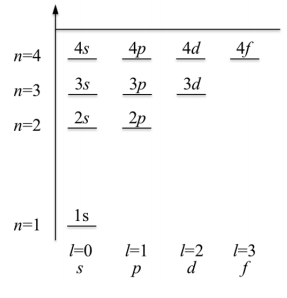
\includegraphics[width=0.3\textwidth]{figures/hyd}
			\caption{The lower energy levels of hydrogen. The degeneracy of $2s$ and $2p$ is evident.}
			\label{fig:hyd}
		\end{figure}
		
		\item \emph{$\braket{j=\frac{9}{2},m=\frac{7}{2},l=4|L_z|j=\frac{9}{2},m=\frac{7}{2},l=4}$ for an electron in a central force field.} \newline
		
		The above is not directly evaluate-able since $\ket{j,l,m}$ is not an eigenstate of $L_z$. Instead I use that
		\begin{equation}
			J_z=J_{1z}+J_{2z}=L_z+S_z.
		\end{equation} 
		In combination with
		\begin{equation}
			J_z\ket{j,l,m}=m\hbar\ket{j,l,m},
		\end{equation} 
		\begin{equation}
			\braket{j,m,l|S_z|j,m,l}|_{j=l\pm\frac{1}{2},m}=\pm\frac{m\hbar}{2l+1},
		\end{equation} 
		where I took the last identity from \citet{Sakurai}[p.338]. The result
		\begin{equation}
			\braket{j,m,l|L_z|j,m,l}=\frac{7}{2}\hbar-\frac{7\hbar}{2(24+1)}=\frac{28}{9}\hbar.
		\end{equation} 
		
		\item \emph{$\braket{singlet,m_s=0|S_z^{(e^-)}-S_z^{(e^+)}|triplet,m_s=0}$ for an $s$-state positronium.} \newline
		
		I use the definitions of the singlet and triplet states. The triplet state
		\begin{equation}
			\vec{S}^2: \quad\lambda_4^{(j=1,m=0)}=\frac{\hbar^2}{2}, \qquad \ket{\lambda_4}=\begin{bmatrix}
				\braket{+,+|\lambda_4} \\
				\braket{+,-|\lambda_4} \\
				\braket{-,+|\lambda_4} \\
				\braket{-,-|\lambda_4} \\
			\end{bmatrix}=\begin{bmatrix}
				0 \\
				1 \\
				1 \\
				0 \\
			\end{bmatrix}.
		\end{equation} 
		The above is also an eigenvector of $S_z$ since $[S_z,\vec{S}^2]=0$. Reformulated in a normalized way
		\begin{equation}
			\ket{j=1,m_s=0}=\frac{1}{\sqrt{2}}\bigg(\ket{+,-}+\ket{-,+}\bigg).
		\end{equation} 
		The singlet state
		\begin{equation}
			\vec{S}^2: \quad\lambda_1^{(j=0,m=0)}=0, \qquad \ket{\lambda_1}=\begin{bmatrix}
				\braket{+,+|\lambda_1} \\
				\braket{+,-|\lambda_1} \\
				\braket{-,+|\lambda_1} \\
				\braket{-,-|\lambda_1} \\
			\end{bmatrix}=\begin{bmatrix}
				0 \\
				1 \\
				-1 \\
				0 \\
			\end{bmatrix}.
		\end{equation} 
		Reformulated in a normalized way
		\begin{equation}
			\ket{j=0,m_s=0}=\frac{1}{\sqrt{2}}\bigg(\ket{+,-}-\ket{-,+}\bigg),
		\end{equation} 
		with the singlet and triplet states expressed in terms of the electron states I can now evaluate the matrix element. I let the operators act on the triplet state
		\begin{equation}
			\begin{split}
				\bigg(S_z^{(e^-)}-S_z^{(e^+)}\bigg)\ket{j=1,m_s=0}&=\bigg(S_z^{(e^-)}-S_z^{(e^+)}\bigg)\frac{1}{\sqrt{2}}\bigg(\ket{+,-}+\ket{-,+}\bigg)\\
				&=\frac{1}{\sqrt{2}}\bigg(\frac{\hbar}{2}+\frac{\hbar}{2}\bigg)\ket{+,-}+\frac{1}{\sqrt{2}}\bigg(-\frac{\hbar}{2}-\frac{\hbar}{2}\bigg)\ket{-,+}\\
				&=\frac{\hbar}{\sqrt{2}}\bigg(\ket{+,-}-\ket{-,+}\bigg)\\
				&=\hbar\ket{j=0,m_s=0}.
			\end{split}
		\end{equation} 
		So, the matrix element is found to be
		\begin{equation}
			\begin{split}
				\hbar&	\braket{j=0,m_s=0|S_z^{(e^-)}-S_z^{(e^+)}|j=1,m_s=0},\\
				&\hbar\braket{j=0,m_s=0|j=0,m_s=0}.
			\end{split}
		\end{equation} 
		
		\item \emph{$\braket{\vec{S}_{1}\cdot\vec{S}_{2}}$ for the ground state of a hydrogen molecule ($H_2$).} \newline
		
		I use that
		\begin{equation}
			\vec{S}_{1}\cdot\vec{S}_{2}=\frac{1}{2}(\vec{S}^2-\vec{S}_1^2-\vec{S}_2^2).
		\end{equation} 
		I take the lowest state to be a spin singlet with $m_s=0$. Thereby $\braket{\vec{S}}=0$ and $\braket{\vec{S}_1^2}=\braket{\vec{S}_2^2}=\frac{1}{2}(\frac{1}{2}+1)\hbar^2=\frac{3}{4}\hbar^2$. Thereby
		\begin{equation}
			\braket{\vec{S}_{1}\cdot\vec{S}_{2}}=\frac{1}{2}(\vec{S}^2-\vec{S}_1^2-\vec{S}_2^2)=\frac{1}{2}(0-\frac{3}{4}\hbar^2-\frac{3}{4}\hbar^2)=-\frac{3}{4}\hbar^2.
		\end{equation} 
	\end{enumerate}
\end{example}

\begin{example}
	\index{TIPT, uniform electric field}
	\index{Hydrogen}
	\emph{A one-electron atom whose GS is non-degenerate is placed in a uniform electric field i the $z$-direction. Obtain an approximate expression for the induced electric dipole moment of the GS by considering the expectation value of $ez$ with respect to the perturbed-state vector computed to first order. Show that the same expression can also be found from the energy shift of the GS computed to second order. Ignore spin.}\newline
	
	In this exercise the GS of a hydrogen-like atom is considered. That is the state $\ket{n,l,m}=\ket{1,0,0}$. Because the electric field is uniform, and in the $z$-direction, the perturbative Hamiltonian is given by
	\begin{equation}
		H'=-ez|\vec{E}|.
	\end{equation} 
	Since the GS is non-degenerate the state vector to first order is given by equation \eqref{correction state}
	\begin{equation}
		\ket{1,0,0}\simeq\ket{(1,0,0)^0}+\sum_{k\neq (1,0,0)^0}\frac{\braket{k^0|H'|(1,0,0)^0}}{E_{(1,0,0)^0}^{(0)}-E_{k}^{(0)}}\ket{k^0}.
	\end{equation} 
	So, the expectation value
	\begin{equation}
		\begin{split}
			\braket{H'}_{1,0,0}&=-e|\vec{E}|\bra{1,0,0}z\ket{1,0,0}\\
			&\simeq-e|\vec{E}|\bigg(-e|\vec{E}|\sum_{k\neq (1,0,0)^0}\frac{\braket{(1,0,0)^0|z|k^0}}{E_{(1,0,0)^0}^{(0)}-E_{k}^{(0)}}\bra{k^0}+\bra{(1,0,0)^0}\bigg)\\
			&\qquad\cdot z\bigg(\ket{(1,0,0)^0}-e|\vec{E}|\sum_{k\neq (1,0,0)^0}\frac{\braket{k^0|z|(1,0,0)^0}}{E_{(1,0,0)^0}^{(0)}-E_{k}^{(0)}}\ket{k^0}\bigg).
		\end{split}
	\end{equation} 	
	To evaluate this I use that $\braket{n',l',m'|z|n,l,m}=0$ unless $l'=l\pm1$ and $m=m'$. So, the element $\braket{(1,0,0)^0|z|(1,0,0)^0}=0$. So, the remainder
	\begin{equation}
		\begin{split}
			\braket{H'}_{1,0,0}&\simeq-e|\vec{E}|\bigg(-2e|\vec{E}|\sum_{k\neq (1,0,0)^0}\frac{|\braket{(1,0,0)^0|z|k^0}|^2}{E_{(1,0,0)^0}^{(0)}-E_{k}^{(0)}}\\
			&+e^2|\vec{E}|^2\sum_{k'\neq (1,0,0)^0}\sum_{k\neq (1,0,0)^0}\frac{\braket{k^0|z|(1,0,0)^0}}{E_{(1,0,0)^0}^{(0)}-E_{k}^{(0)}}\frac{\braket{(1,0,0)^0|z|k'^0}}{E_{(1,0,0)^0}^{(0)}-E_{k'}^{(0)}}\bra{k'^0}z\ket{k^0}\bigg).
		\end{split}
	\end{equation} 
	The last term vanishes since $0\neq \braket{k^0|z|(1,0,0)^0}$ if $k=n,1,0$ and likewise for $\braket{(1,0,0)^0|z|k'^0}$. However, $\bra{k'^0}z\ket{k^0}=0$ in these cases. Therefore
	\begin{equation}
		\braket{H'}_{1,0,0}\simeq 2e^2|\vec{E}|^2\sum_{k\neq (1,0,0)^0}\frac{|\braket{(1,0,0)^0|z|k^0}|^2}{E_{(1,0,0)^0}^{(0)}-E_{k}^{(0)}}.
	\end{equation} 
\end{example}

\begin{example}
	\index{TIPT, two-state system}
	\emph{The Hamiltonian for a two-state system can be written as}
	\begin{equation}
		H=H_0+H'\doteq\begin{bmatrix}
			E_1^{(0)} & 0 \\
			0 & E_2^{(0)}\\
		\end{bmatrix}+\lambda\begin{bmatrix}
			0 &  \Delta \\
			\Delta & 0\\
		\end{bmatrix}=\begin{bmatrix}
			E_1^{(0)} & \lambda \Delta \\
			\lambda \Delta & E_2^{(0)}\\
		\end{bmatrix}.
	\end{equation} 
	\emph{The energy eigenfunctions for the unperturbed problems ($\lambda=0$) are given by}
	\begin{equation}
		\ket{\phi_1^{(0)}}=\begin{bmatrix}
			1 \\
			0 \\
		\end{bmatrix} \quad \mbox{,} \quad \ket{\phi_2^{(0)}}=\begin{bmatrix}
			0 \\
			1 \\
		\end{bmatrix}.
	\end{equation} 
	
	\begin{enumerate}
		\item \emph{Solve this problem exactly to find the energy eigenvectors $\ket{E_{1,2}}$ and the energy eigenvalues $E_{1,2}$.}\newline
		
		The problem can be set up as a matrix equation on the form
		\begin{equation}
			H\vec{x}=E\vec{x}.
			\label{eq24}
		\end{equation} 
		Cf. Cramers rule (equation \eqref{cramer1}) this only has non-trivial solutions when
		\begin{equation}
			det(H-EI)=0.
		\end{equation} 
		From this I find the eigenvalues to be
		\begin{equation}
			E_{1,2}=\frac{E_1^{(0)}+E_2^{(0)}\mp\sqrt{(E_2^{(0)}-E_1^{(0)})^2+4\lambda^2\Delta^2}}{2}.
			\label{eq26}
		\end{equation} 
		By insertion of the eigenvalues into equation \eqref{eq24} the components of the eigenvectors can be found. This will result in two non-independent equations, and so one of the coefficients can be chosen to be 1 in order to determine the other. The unnormalized eigenvectors are therefore
		\begin{equation}
			\ket{E_{1}}=\begin{bmatrix}
				1 \\
				\frac{E_{1}-E_1^{(0)}}{\lambda\Delta} \\
			\end{bmatrix} \quad \mbox{;}\quad \ket{E_{2}}=\begin{bmatrix}
				\frac{E_{2}-E_2^{(0)}}{\lambda\Delta} \\
				1 \\
			\end{bmatrix}.
			\label{eq27}
		\end{equation} 
		The reason for the odd way to list the eigenvectors is to compare with the results from perturbation theory easily.\newline
		
		\item \emph{Assuming that $\lambda |\Delta|\ll |E_1^{(0)}-E_2^{(2)}|$, solve the same problem using time-independent perturbation theory up to first order in the energy eigenfunctions and up to second order in the energy eigenvalues. Compare with the exact results.}\newline
		
		From equation \eqref{correction energy}
		\begin{equation}
			\Delta E_n= \braket{n^0|H'|n^0}+\sum_{k\neq n}\frac{|\braket{k^0|H'|n^0}|^2}{E_n^0-E_k^0}+...,
		\end{equation} 
		where $\braket{n^0|H'|n^0}$ is the diagonal elements of the \emph{potential} matrix given by
		\begin{equation}
			H'\doteq\begin{bmatrix}
				0 & \lambda \Delta \\
				\lambda \Delta & 0\\
			\end{bmatrix}.
		\end{equation} 
		Hence the diagonal elements are zero, and so the first order correction to the energy (for both energy eigenvalues) is zero. For the second order correction
		\begin{equation}
			\begin{split}
				&\Delta E_1=\lambda \braket{1^0|H'|1^0}+\lambda^2\sum_{k\neq 1}\frac{|\braket{k^0|H'|1^0}|^2}{E_1^0-E_k^0}+...\\
				&\qquad=\lambda^2\frac{|\Delta|^2}{E_1^{(0)}-E_2^{(0)}},\\
				&\Delta E_2= \braket{2^0|H'|2^0}+\sum_{k\neq 1}\frac{|\braket{k^0|H'|2^0}|^2}{E_2^0-E_k^0}+...\\
				&\qquad=\lambda^2\frac{|\Delta|^2}{E_2^{(0)}-E_1^{(0)}}+....
			\end{split}
		\end{equation} 
		To compare with the exact result I consider $E_1$ as an example. I can rewrite it as\footnote{where I use $\lambda |\Delta|\ll |E_1^{(0)}-E_2^{(2)}|$ to Taylor expand the square root to second order; $\sqrt{1+x}=1+\frac{x}{2}+...$}
		\begin{equation}
			\begin{split}
				E_{1}&=\frac{E_1^{(0)}+E_2^{(0)}}{2}+\frac{E_2^{(0)}-E_1^{(0)}}{2}\sqrt{1+\frac{4\lambda^2\Delta^2}{(E_2^{(0)}-E_1^{(0)})^2}}\\
				&\simeq \frac{E_1^{(0)}+E_2^{(0)}}{2}+\frac{E_2^{(0)}-E_1^{(0)}}{2}\bigg(1+\frac{2\lambda^2\Delta^2}{(E_2^{(0)}-E_1^{(0)})^2}\bigg)\\
				&=E_1^{(0)}+\frac{\lambda^2\Delta^2}{E_1^{(0)}-E_2^{(0)}},
			\end{split}
		\end{equation} 
		which is the same as the exact case\footnote{A completely analogous procedure can be performed for $E_2$.}. For the eigenstates
		\begin{equation}
			\begin{split}
				&\ket{E_1}=\ket{E_1^{(0)}}+\lambda\sum_{k\neq 1}^{}\frac{\braket{k'^0|H'|E_1^{(0)}}}{E_1^{(0)}-E_{k'}^{(0)}}\ket{k^0}+\dots\\
				&\qquad=\ket{E_1^{(0)}}+\frac{\lambda\Delta}{E_1^{(0)}-E_{2}^{(0)}}\ket{E_2^{(0)}}+\dots,\\
				&\ket{E_2}=\ket{E_2^{(0)}}+\lambda\sum_{k\neq 1}^{}\frac{\braket{k'^0|H'|E_2^{(0)}}}{E_2^{(0)}-E_{k'}^{(0)}}\ket{k^0}+\dots\\
				&\qquad=\ket{E_2^{(0)}}+\frac{\lambda\Delta}{E_2^{(0)}-E_{1}^{(0)}}\ket{E_1^{(0)}}+\dots.
			\end{split}
			\label{eq25}
		\end{equation} 
		Inserting the eigenvalues in the exact results and Taylor expanding the square roots to second order will reveal the eigenvectors above found from perturbation theory
		\begin{equation}
			\begin{split}
				\ket{E_{1}}&\doteq\begin{bmatrix}
					1 \\
					\frac{E_{1}-E_1^{(0)}}{\lambda\Delta} \\
				\end{bmatrix}\\
				&=\begin{bmatrix}
					1 \\
					\frac{1}{\lambda\Delta}\bigg(\frac{E_1^{(0)}+E_2^{(0)}}{2}-\frac{(E_2^{(0)}-E_1^{(0)})}{2}\sqrt{1+\frac{4\lambda^2\Delta^2}{(E_2^{(0)}-E_1^{(0)})^2}}-E_1^{(0)}\bigg) \\
				\end{bmatrix}\\
				&\simeq\begin{bmatrix}
					1 \\
					\frac{1}{\lambda\Delta}\bigg(\frac{E_1^{(0)}+E_2^{(0)}}{2}-\frac{E_2^{(0)}-E_1^{(0)}}{2}(1+\frac{2\lambda^2\Delta^2}{(E_2^{(0)}-E_1^{(0)})^2})-E_1^{(0)}\bigg) \\
				\end{bmatrix}\\
				&=\begin{bmatrix}
					1 \\
					-\frac{1}{\lambda\Delta}\frac{E_2^{(0)}-E_1^{(0)}}{2}\frac{2\lambda^2\Delta^2}{(E_2^{(0)}-E_1^{(0)})^2} \\
				\end{bmatrix}=\begin{bmatrix}
					1 \\
					\frac{\lambda\Delta}{E_1^{(0)}-E_2^{(0)}} \\
				\end{bmatrix},
			\end{split}
		\end{equation} 
		which is identical to equation \eqref{eq25}.\newline
		
		\item \emph{Suppose the two unperturbed energy levels are "almost degenerate", i.e. $\lambda |\Delta|\gg |E_1^{(0)}-E_2^{(2)}|$. Show that the exact results obtained earlier closely resemble what you would expect by applying degenerate perturbation theory to this problem with $E_1^{(0)}=E_2^{(0)}=E^{(0)}$.}\newline
		
		In this case the Hamiltonian will be on the form
		\begin{equation}
			\begin{split}
				H&=H_0+H'\\
				&\doteq E^{(0)}\begin{bmatrix}
					1 & 0 \\
					0 & 1\\
				\end{bmatrix}+\lambda \Delta\begin{bmatrix}
					0 & 1 \\
					1 & 0\\
				\end{bmatrix}.
			\end{split}
		\end{equation} 
		I diagonalize $\lambda H'$. The eigenvalues are the first order correction to the energy whereas the eigenvectors are the eigenvectors of the energy levels. I find
		\begin{equation}
			E_1=E^{(0)}+\lambda\Delta \quad \mbox{and} \quad E_2=E^{(0)}-\lambda\Delta,
		\end{equation} 
		\begin{equation}
			\ket{E_1}=\begin{bmatrix}
				1 \\
				1 \\
			\end{bmatrix} \quad \mbox{and} \quad \ket{E_2}=\begin{bmatrix}
				-1 \\
				1 \\
			\end{bmatrix}.
		\end{equation} 
		Letting $E_1^{(0)}=E_2^{(0)}=E^{(0)}$ in equation \eqref{eq26} results in $E_i=E^{(0)}\pm\lambda\Delta$ just as above. Using $E_i=E^{(0)}\pm\lambda\Delta$ in equation \eqref{eq27} results in $\ket{E_i}=\begin{bmatrix}
			\pm1 \\
			1 \\
		\end{bmatrix}$ - just as above. Therefore, in the limit of almost degenerate energy levels, the exact method and the degenerate perturbation theory reveals the same result. 
		
	\end{enumerate}
\end{example}

\begin{example}
	\label{electric dipole}
	To illustrate the calculations required, I analyze the semi classical case of an electric dipole. I take $H'(t)$ to be on the form
	\begin{equation}
		H'(t)=-\vec{\mu}\cdot\vec{E}_0cos(\omega t),
		\label{semi clas}
	\end{equation} 
	where $\vec{E}_0$ is the magnitude of the electrical field, and unrelated to the energy, $E_n$. By using equation \eqref{semi clas} in \eqref{coef} I find the squared amplitude to be
	\begin{equation}
		|c^1_{b_0}(t_p)|^2=\bigg(\frac{E_0}{\hbar}\bigg)^2|\bra{b_0}\mu\ket{a_0}|^2\bigg|\int_{0}^{t_p}(-)e^{i\omega_{b_0a_0}t}cos(\omega t)dt\bigg|^2.
		\label{prob}
	\end{equation} 
	I define the integral as $I$ and evaluate it
	\begin{equation}
		\begin{split}
			I
			&=\int_{0}^{t_p}(-)e^{i\omega_{b_0a_0}t}cos(\omega t)dt\\
			&=\int_{0}^{t_p}(-)e^{i\omega_{b_0a_0}t}\bigg(\frac{e^{i\omega t}+e^{-i\omega t}}{2}\bigg)dt\\
			&=-\frac{1}{2}\int_{0}^{t_p}e^{i\omega_{b_0a_0}t}(e^{i\omega t}+e^{-i\omega t})dt\\
			&=-\frac{1}{2}\bigg(\int_{0}^{t_p}e^{i(\omega_{b_0a_0}+\omega)t}dt+\int_{0}^{t_p}e^{i(\omega_{b_0a_0}-\omega)t}dt\bigg)\\
			&=-\frac{1}{2}\bigg(\frac{e^{i(\omega_{b_0a_0}+\omega)t_p}-1}{i(\omega_{b_0a_0}+\omega)}+\frac{e^{i(\omega_{b_0a_0}-\omega)t_p}-1}{i(\omega_{b_0a_0}-\omega)}\bigg)\\
			&=\frac{1}{2i}\bigg(\frac{1-e^{i(\omega_{b_0a_0}+\omega)t_p}}{\omega_{b_0a_0}+\omega}+\frac{1-e^{i(\omega_{b_0a_0}-\omega)t_p}}{\omega_{b_0a_0}-\omega}\bigg).
		\end{split}
		\label{calc}
	\end{equation} 
	Using equation \eqref{calc} in \ref{prob} and letting the magnitude-operator absorb the imaginary unit, I find
	\begin{equation}
		|c^1_{b_0}(t_p)|^2=\bigg(\frac{E_0}{2\hbar}\bigg)^2|\bra{b_0}\mu\ket{a_0}|^2\bigg|\frac{1-e^{i(\omega_{b_0a_0}+\omega)t_p}}{\omega_{b_0a_0}+\omega}+\frac{1-e^{i(\omega_{b_0a_0}-\omega)t_p}}{\omega_{b_0a_0}-\omega}\bigg|^2.
	\end{equation} 
	To get considerable probability, the denominator needs to explode. This gives rise to the criterion for a large transition probability
	\begin{equation}
		\omega\simeq|\omega_{b_0a_0}|.
		\label{criterion}
	\end{equation} 
	Equation \eqref{criterion} causes the denominator in one of the fractions to "explode" -the other one does not explode, and can therefore be neglected. I find 
	\begin{equation}
		\begin{split}
			&\omega\simeq\omega_{b_0a_0} \quad |c^1_{b_0}(t_p)|^2\simeq\bigg(\frac{E_0}{2\hbar}\bigg)^2|\bra{b_0}\mu\ket{a_0}|^2\bigg|\frac{sin(\frac{\omega_{b_0a_0}-\omega}{2}t_p)}{\frac{\omega_{b_0a_0}-\omega}{2}}\bigg|^2,\\
			&\omega\simeq-\omega_{b_0a_0} \quad |c^1_{b_0}(t_p)|^2\simeq\bigg(\frac{E_0}{2\hbar}\bigg)^2|\bra{b_0}\mu\ket{a_0}|^2\bigg|\frac{sin(\frac{\omega_{b_0a_0}+\omega}{2}t_p)}{\frac{\omega_{b_0a_0}+\omega}{2}}\bigg|^2.
		\end{split}
		\label{trans1}
	\end{equation} 
	Using the definition of $\omega_{m_0n_0}=\frac{E_{m_0}-E_{n_0}}{\hbar}$
	\begin{equation}
		\begin{split}
			&\omega_{m_0n_0}>0:\quad\omega_{m_0n_0}=\frac{E_{b_0}-E_{a_0}}{\hbar}>0\\
			&\qquad \Rightarrow E_{b_0}>E_{a_0}\Rightarrow \mbox{Absorption of $1$ photon},\\
			&\omega_{m_0n_0}<0:\quad\omega_{m_0n_0}=\frac{E_{b_0}-E_{a_0}}{\hbar}<0\\
			&\qquad  \Rightarrow E_{b_0}<E_{a_0}\Rightarrow \mbox{Emission of $1$ photon}.
		\end{split}
	\end{equation} 
	In equation \eqref{trans1} $\omega_{b_0a_0}\pm\omega$ is raised to the second power and sine is an odd function to the second power\footnote{Meaning that $sin(-x)=-sin(x)$.}. This means that the probability for absorption and emission of $1$ photon is the same. The probability depends on the perturbation time and the frequency of the electromagnetic wave. The dependency of the perturbation time is shown in figure \ref{fig:pertub2}.
	\begin{figure}[ht]
		\captionsetup{width=1\textwidth}
		\centering
		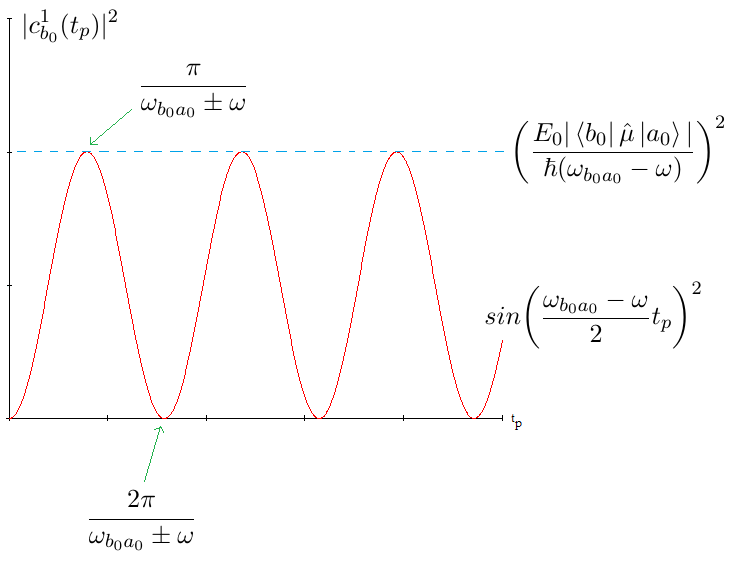
\includegraphics[width=0.6\textwidth]{figures/tipertub1}
		\caption{The transition probability as a function of perturbation time.}
		\label{fig:pertub2}
	\end{figure}
	As is evident from figure \ref{fig:pertub2}; the transition probability varies periodically with the perturbation time. To have greatest possibility of a transition, the perturbation time must be given by
	\begin{equation}
		t_p=\frac{(2k+1)\pi}{\omega_{b_0a_0}\pm\omega},
	\end{equation} 
	where $k=1,2,3,...$. The dependency of the transition probability on the angular frequency of the electromagnetic wave is shown in figure \ref{fig:pertub3}. Here equation \eqref{trans1} is rewritten to
	\begin{equation}
		\omega\simeq\omega_{b_0a_0} \quad |c^1_{b_0}(t_p)|^2\simeq\bigg(\frac{E_0|\bra{b_0}\mu\ket{a_0}|}{2\hbar}\bigg)^2t_p^2\bigg|sinc\bigg(\frac{\omega_{b_0a_0}-\omega}{2}t_p\bigg)\bigg|^2.
	\end{equation} 
	\begin{figure}[H]
		\captionsetup{width=1\textwidth}
		\centering
		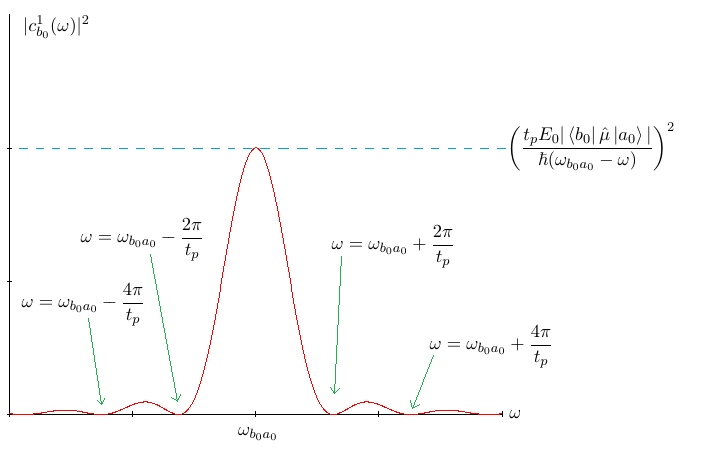
\includegraphics[width=0.6\textwidth]{figures/tipertub2}
		\caption{The transition probability as a function of the angular frequency of the electromagnetic wave.}
		\label{fig:pertub3}
	\end{figure}
	As is evident from figure \ref{fig:pertub3}; the transition probability peaks around $\omega_{b_0a_0}$. Thus, in order to maximize the transition probability, the time, $t_p$, and angular frequency, $\omega$, must have certain values.
\end{example}


\begin{example}
	\index{TDPT, SHO}
	\index{State vector in TDPT}
	\index{Expectation value in TDPT}
	\emph{Consider a one-dimensional simple harmonic oscillator whose classical angular frequency is $\omega_0$. For $t<0$ it is known to be in the ground state. For $t>0$ there is also a time-dependent potential given by}
	\begin{equation}
		H'(t)=F_0xcos(\omega t),
	\end{equation} 	
	\emph{where $F_0$ is constant in both space and time. Obtain an expression for the expectation value $\braket{x}$ as a function of time using time-dependent perturbation theory to lowest non-vanishing order. Is this procedure valid for $\omega\simeq \omega_0$?}\newline
	
	What is to be evaluated is
	\begin{equation}
		\braket{x}=\braket{0(t)|x|0(t)},
	\end{equation} 
	where
	\begin{equation}
		\ket{0(t)}=\sum_{n}c_n(t)e^{-i\frac{H_0t}{\hbar}}\ket{n}, \quad c_n(t)=c_n^{(0)}+c_n^{(1)}(t)+c_n^{(2)}(t)+\dots.
	\end{equation} 
	To first order; $c_0(t)=c_0^{(0)}$ since $\braket{0|x|0}$ from the first order term ($c_0^{(1)}$) is zero. For the first energy level;$c_1(t)=c_1^{(0)}+c_1^{(1)}(t)$ where $c_1^{0}=0$ cf. the initial condition that the state at $t=0$ is in the ground state. The rest of the coefficients, $c_n(t)$ ($n\geq2$) vanish since
	\begin{equation}
		\braket{n'|x|n}=\sqrt{\frac{\hbar}{2M\omega_0}}\bigg(\sqrt{n+1}\delta_{n',+1}+\sqrt{n}\delta_{n',n-1}\bigg).
		\label{hest}
	\end{equation} 
	Therefore
	\begin{equation}
		\ket{0(t)}=c_0^{(0)}e^{-\frac{1}{2}i\omega t}\ket{0}+c_1^{(1)}e^{-\frac{3}{2}i\omega t}\ket{1}.
	\end{equation} 
	Since at $t=0$ the state is in the ground state; $c_0^{0}\simeq1$. For the first excited state (from equation \eqref{coef})
	\begin{equation}
		\begin{split}
			c^1_{n}(t)&=\frac{1}{i\hbar}\int_{0}^{t}\bra{n}H'(t')\ket{0}e^{i\omega_{0}t'}dt'\\
			&=\frac{F_0\bra{n}x\ket{0}}{i\hbar}\int_{0}^{t}cos(\omega t')e^{i\omega_{0}t'}dt'\\
			&=\frac{F_0\bra{n}x\ket{0}}{i\hbar}\bigg(\int_{0}^{t}cos(\omega t')cos(\omega_0t')dt'+i\int_{0}^{t}cos(\omega t')sin(\omega_0t')dt'\bigg)\\
			&=\frac{F_0\bra{n}x\ket{0}}{2\hbar}\bigg(\frac{e^{-i(\omega-\omega_0)t}-1}{\omega-\omega_0}-\frac{e^{i(\omega+\omega_0)t}-1}{\omega+\omega_0}\bigg).\\
		\end{split}
	\end{equation} 
	So, to first order the expectation value can be written as
	\begin{equation}
		\begin{split}
			\braket{0(t)|x|0(t)}&=(\bra{1}e^{\frac{i3\hbar\omega_0t}{2}}c_1^{(1)*}+\bra{0}e^{\frac{i\hbar\omega_0t}{2}}c_0^{(0)})\\
			&\quad\cdot x(c_0^{(0)*}e^{\frac{-i\hbar\omega_0t}{2}}\ket{0}+c_1^{(1)}e^{\frac{-i3\hbar\omega_0t}{2}}\ket{1})\\
			&=\braket{1|x|0}e^{i\omega_0t}c_1^{(1)*}+\braket{0|x|1}e^{-i\omega_0t}c_1^{(1)},
		\end{split}
	\end{equation} 
	where equation \eqref{hest} has been used again to make the terms with $\braket{n|x|n}$ vanish. Thereby
	\begin{equation}
		\begin{split}
			\braket{x}&=\frac{F_0}{M}\frac{cos(\omega t)-cos(\omega_0t)}{\omega^2-\omega_0^2},
		\end{split}
	\end{equation} 
	where I have used that $\braket{1|x|0}=\sqrt{\frac{\hbar}{2M\omega_0}}$.
\end{example}

\begin{example}
	\index{TDPT, SHO}
	\index{Transition probability}
	\emph{A one-dimensional SHO is in its ground state for $t<0$. For $t\geq0$ it is subjected to a time.-dependent but spatially uniform force in the x-direction}
	\begin{equation}
		\vec{F}(t)=F_0e^{-\frac{t}{\tau}}\begin{bmatrix}
			1\\0\\0\\
		\end{bmatrix}.
	\end{equation} 
	
	\begin{enumerate}
		\item \emph{Using TDPT to first order, obtain the probability of finding the oscillator in its first excited state for $t>0$. Show that in the limit of $t\Rightarrow \infty$ the result is independent of time. Is this reasonable or surprising?} \newline
		
		First I convert the perturbative force into a perturbative potential which I can add to the Hamiltonian. I use that $\vec{F}=-\vec{\nabla}\cdot V(t)$. Hereby
		\begin{equation}
			V(t)=H'(t)=-F_0xe^{-\frac{t}{\tau}}.
		\end{equation} 
		The transition probability
		\begin{equation}
			P_{0\Rightarrow 1}(t)\simeq|c_1^{(1)}(t)|^2,
		\end{equation} 
		where
		\begin{equation}
			\begin{split}
				c_1^{(1)}(t)&=\frac{1}{i\hbar}\int_{0}^{t}\braket{1|H'(t')|0}e^{i\omega_{10}t'}dt'\\
				&=-\frac{\braket{1|x|0}F_0}{i\hbar}\int_{0}^{t}e^{t'(i\omega_{10}-\frac{1}{\tau})}dt'\\
				&=-\frac{\braket{1|x|0}F_0}{i\hbar}\frac{e^{t(i\omega_{10}-\frac{1}{\tau})}-1}{(i\omega_{10}-\frac{1}{\tau})}.\\
			\end{split}
		\end{equation} 
		By insertion
		\begin{equation}
			\begin{split}
				P_{0\Rightarrow 1}(t)&\simeq\bigg|-\frac{\braket{1|x|0}F_0}{i\hbar}\frac{e^{t(i\omega_{10}-\frac{1}{\tau})}-1}{(i\omega_{10}-\frac{1}{\tau})}\bigg|^2\\
				&=\frac{|\braket{1|x|0}|^2F_0^2}{\hbar^2}\bigg|\frac{e^{t(i\omega_{10}-\frac{1}{\tau})}-1}{(i\omega_{10}-\frac{1}{\tau})}\bigg|^2\\
				&=\frac{|\braket{1|x|0}|^2F_0^2}{\hbar^2}\frac{e^{t(i\omega_{10}-\frac{1}{\tau})}-1}{(i\omega_{10}-\frac{1}{\tau})}\frac{e^{t(-i\omega_{10}-\frac{1}{\tau})}-1}{(-i\omega_{10}-\frac{1}{\tau})}\\
				&=\frac{|\braket{1|x|0}|^2F_0^2}{\hbar^2}\frac{e^{-\frac{2t}{\tau}}-e^{-\frac{t}{\tau}}2cos(\omega_{10}t)+1}{\omega_{10}^2+\frac{1}{\tau^2}}.\\
			\end{split}
		\end{equation} 
		In the limit of $t\Rightarrow \infty$
		\begin{equation}
			\lim\limits_{t\Rightarrow\infty}(P_{0\Rightarrow 1}(t))\simeq\frac{|\braket{1|x|0}|^2F_0^2}{\hbar^2}\frac{1}{\omega_{10}^2+\frac{1}{\tau^2}}.
		\end{equation} 
		This makes sense since the perturbation will vanish in this limit. 
		
		\item \emph{Can higher states be the destination of the perturbation?}\newline
		
		Not to first order since $\braket{n'|x|0}=\sqrt{\frac{\hbar}{2M\omega}}\delta_{n',1}$. To second order (cf. equation \eqref{second order})
		\begin{equation}
			\begin{split}
				c^{(2)}_{b_0}(t)&=-\frac{1}{\hbar^2}\int_{0}^{t}\bra{b_0}H'(t'')\ket{1}e^{i\omega_{b_0,1}t''}\int_{0}^{t''}\bra{1}H'(t')\ket{0}e^{i\omega_{n_0,0}t'}dt'dt'',
				\\
			\end{split}
		\end{equation} 
		where I used that only $\bra{1}H'(t')\ket{0}\neq0$ which also requires $b_0=2$(!). This expression is in general non-zero, and so there is a finite transition probability to the second excited state.
	\end{enumerate}
\end{example}
\begin{example}
	\index{TDPT, SHO}
	\index{Transition probability}
	\emph{Consider a particle bound in a SHO potential. Initially ($t<0$) it is in the GS. At $t=0$ a perturbation is turned on. the perturbation is given by}
	\begin{equation}
		H'(x,t)=Ax^2e^{-\frac{t}{\tau}}.
	\end{equation} 
	\emph{calculate the probability that after a long time, $t\gg\tau$, the system will have made a transition to a given excited state. Consider all final states.}\newline
	
	Since $c_n^{(1)}\propto \braket{n^0|x^2|0^0}$ I consider these matrix elements. Cf. equation \eqref{shit}
	\begin{equation}
		\begin{split}
			\braket{n^0|x^2|0^0}&=\frac{\hbar}{2M\omega}\bigg(\braket{n^0|a^\dagger a|0^0}+\braket{n^0|a^\dagger a^\dagger|0^0}+\braket{n^0|aa^\dagger|0^0}+\braket{n^0|aa|0^0}\bigg)\\
			&=\frac{\hbar}{2M\omega}\bigg(\braket{n^0|a^\dagger a^\dagger|0^0}\delta_{n,2}+\braket{n^0|aa^\dagger|0^0}\delta_{n,0}\bigg).\\
		\end{split}
	\end{equation} 
	Here only the GS and the second excited state reveals any results. So, the relevant probability here is given by
	\begin{equation}
		P_{0\Rightarrow 2}(t)=|\braket{2|\alpha(t)}|^2=|c_2^{(1)}(t)|^2,
	\end{equation} 
	where
	\begin{equation}
		\begin{split}
			c_2^{(1)}(t)&=\frac{1}{i\hbar}\int_{0}^{t}\braket{2|H'(t')|0}e^{i\omega_{20}t'}dt'\\
			&=-\frac{\braket{2|x^2|0}A}{i\hbar}\int_{0}^{t}e^{t'(i\omega_{20}-\frac{1}{\tau})}dt'\\
			&=-\frac{\braket{2|x^2|0}A}{i\hbar}\frac{e^{t(i\omega_{20}-\frac{1}{\tau})}-1}{(i\omega_{20}-\frac{1}{\tau})}.\\
		\end{split}
	\end{equation} 
	By insertion
	\begin{equation}
		\begin{split}
			P_{0\Rightarrow 2}(t)&\simeq\bigg|-\frac{\braket{2|x^2|0}A}{i\hbar}\frac{e^{t(i\omega_{20}-\frac{1}{\tau})}-1}{(i\omega_{20}-\frac{1}{\tau})}\bigg|^2\\
			&=\frac{|\braket{2|x^2|0}|^2A^2}{\hbar^2}\bigg|\frac{e^{t(i\omega_{20}-\frac{1}{\tau})}-1}{(i\omega_{20}-\frac{1}{\tau})}\bigg|^2\\
			&=\frac{|\braket{2|x^2|0}|^2A^2}{\hbar^2}\frac{e^{t(i\omega_{20}-\frac{1}{\tau})}-1}{(i\omega_{20}-\frac{1}{\tau})}\frac{e^{t(-i\omega_{20}-\frac{1}{\tau})}-1}{(-i\omega_{20}-\frac{1}{\tau})}\\
			&=\frac{|\braket{2|x^2|0}|^2A^2}{\hbar^2}\frac{e^{-\frac{2t}{\tau}}-e^{-\frac{t}{\tau}}2cos(\omega_{20}t)+1}{\omega_{20}^2+\frac{1}{\tau^2}}.\\
		\end{split}
	\end{equation} 
	In the limit of $t\Rightarrow \infty$
	\begin{equation}
		\lim\limits_{t\Rightarrow\infty}(P_{0\Rightarrow 2}(t))\simeq\frac{|\braket{2|x^2|0}|^2A^2}{\hbar^2}\frac{1}{\omega_{20}^2+\frac{1}{\tau^2}}.
	\end{equation} 
	This makes sense since the perturbation will vanish in this limit.
\end{example}


\begin{example}
	\index{TDPT, two-state system}
	\emph{The unperturbed Hamiltonian of a two-state system is represented by}
	\begin{equation}
		H_0\doteq\begin{bmatrix}
			E_1^{(0)} & 0\\
			0 & E_2^{(0)} \\ 
		\end{bmatrix}.
	\end{equation} 
	\emph{The two state system is perturbed by}
	\begin{equation}
		H'(t)\doteq\begin{bmatrix}
			0 & \lambda cos(\omega t)\\
			\lambda cos(\omega t) & 0 \\ 
		\end{bmatrix},
	\end{equation} 
	\emph{where $\lambda$ is real.} \newline
	
	\begin{enumerate}
		\item \emph{At $t=0$ the system in known to be in the first state, represented by}
		\begin{equation}
			\ket{1}=\begin{bmatrix}
				1\\
				0 \\ 
			\end{bmatrix}.
		\end{equation} 
		\emph{Using TDPT and assuming that $E_1^{(0)}-E_2^{(0)}$ is not close to $\pm \hbar \omega$, derive an expression for the probability that the system is found in the second state represented by}
		\begin{equation}
			\ket{2}=\begin{bmatrix}
				0\\
				1 \\ 
			\end{bmatrix}
		\end{equation} 
		\emph{as a function of time.}\newline
		
		I use that
		\begin{equation}
			P_{1\Rightarrow 2}(t)=|\braket{2|\alpha(t)}|^2,
		\end{equation} 		
		where $\ket{\alpha(t)}$ is a general state vector described by
		\begin{equation}
			\ket{\alpha(t)}=c_1(t)e^{-\frac{iE_1^{(0)}t}{\hbar}}\ket{1}+c_2(t)e^{-\frac{iE_2^{(0)}t}{\hbar}}\ket{2}.
		\end{equation} 
		Since $\ket{1}$ and $\ket{2}$ are orthogonal the probability reduces to
		\begin{equation}
			P_{1\Rightarrow 2}(t)=|\braket{2|\alpha(t)}|^2=\big|c_2(t)e^{-\frac{iE_2^{(0)}t}{\hbar}}\big|^2=|c_2(t)|^2.
		\end{equation} 
		To first order
		\begin{equation}
			\begin{split}
				c_2^{(1)}(t)&=\frac{1}{i\hbar}\int_{0}^{t}\braket{2|H'(t')|1}e^{i\omega_{21}t'}dt'\\
				&=\frac{\lambda}{i\hbar}\int_{0}^{t}cos(\omega t)e^{i\omega_{21}t'}dt'.\\
			\end{split}
		\end{equation} 
		From this the probability can be found; use partial integration or see section \ref{electric dipole}.
		
	\end{enumerate}
\end{example}

\begin{example}
	\index{TDPT, two-state system}
	\emph{Consider a two-level system with $E_1<E_2$. There is a time-dependent potential that connects the two levels as follows}
	\begin{equation}
		H'\doteq\begin{bmatrix}
			0 & \gamma e^{i\omega t} \\
			\gamma e^{-i\omega t} & 0\\
		\end{bmatrix},
	\end{equation} 	
	\emph{where $\gamma$ is a real constant. At $t=0$, it is known that only the lower level is populated (i.e. $c_1(0)=1$, $c_2(0)=0$).}\newline
	
	\begin{enumerate}
		\item \emph{Find $|c_1(t)|^2$ and $|c_2(t)|^2$ for $t>0$ by exactly solving the coupled differential equation}
		\begin{equation}
			i\hbar\frac{\partial c_k}{\partial t}=\sum_{n=1}^{2}\braket{k|H'(t)|n}e^{i\omega_{kn}t}c_n,
		\end{equation}		
		\emph{where $k=1,2$.}\newline
		
		I use that
		\begin{equation}
			i\hbar\frac{\partial c_1}{\partial t}=\gamma e^{i(\omega+\omega_{12}) t}c_2,
		\end{equation} 
		\begin{equation}
			i\hbar\frac{\partial c_2}{\partial t}=\gamma e^{i(\omega_{21}-\omega) t}c_1.
			\label{eq28}
		\end{equation} 
		I isolate $c_1$ from the second equation, differentiate it and insert it in the first equation. I find
		\begin{equation}
			\frac{\partial^2 c_2}{\partial t^2}+i(\omega-\omega_{21}))\frac{\partial c_2}{\partial t}+\frac{\gamma^2}{\hbar^2} e^{i(\omega_{12}+\omega_{21})t}c_2=0.
		\end{equation} 
		Using now that $\omega_{12}=-\omega_{21}$
		\begin{equation}
			\frac{\partial^2 c_2}{\partial t^2}+i(\omega-\omega_{21})\frac{\partial c_2}{\partial t}+\frac{\gamma^2}{\hbar^2}c_2=0.
		\end{equation} 
		Using the auxiliary equation I identify
		\begin{equation}
			\begin{split}
				&a=1,\\
				&b=i(\omega-\omega_{21}),\\
				&c=\frac{\gamma^2}{\hbar^2}.\\
			\end{split}
		\end{equation} 
		Using then that
		\begin{equation}
			D=b^2-4ac=-(\omega-\omega_{21})^2-\frac{4\gamma^2}{\hbar^2}<0,
		\end{equation} 
		the solution is on the form
		\begin{equation}
			c_2(t)=Acos(\omega_0t)+Bsin(\omega_0t),
		\end{equation} 
		where from $c_2(0)=0\Rightarrow A=0$, and $\omega_0$ is found from
		\begin{equation}
			r=\frac{-b\pm\sqrt{b^2-4ac}}{2a}=k\pm i\omega_0.
		\end{equation} 
		Evaluating $r$
		\begin{equation}
			\begin{split}
				r&=0\pm\frac{i}{2}\bigg(\sqrt{(\omega-\omega_{21})^2+\frac{4\gamma^2}{\hbar^2}}-(\omega-\omega_{21})\bigg)\\
				&\Rightarrow \omega_0=\frac{1}{2}\bigg(\sqrt{(\omega-\omega_{21})^2+\frac{4\gamma^2}{\hbar^2}}-(\omega-\omega_{21})\bigg).
			\end{split}
		\end{equation} 
		So
		\begin{equation}
			c_2(t)=Bsin(\omega_0t).
		\end{equation} 
		From using this in equation \eqref{eq28}
		\begin{equation}
			c_1(t)=\frac{i\hbar}{\gamma e^{i(\omega_{21}-\omega)t}}\frac{\partial c_2(t)}{\partial t}=\frac{iB\omega_0\hbar}{\gamma}e^{i(\omega-\omega_{21})t}cos(\omega_0t),
		\end{equation} 
		since $c_1(0)=1\Rightarrow B=-\frac{i\gamma}{\omega_0\hbar}$. So
		\begin{equation}
			\begin{split}
				&c_1(t)=e^{-i(\omega+\omega_{21})t}cos(\omega_0t),\\
				&c_2(t)=-\frac{i\gamma}{\omega_0\hbar}sin(\omega_0t).\\
			\end{split}
		\end{equation} 
		The probabilities
		\begin{equation}
			\begin{split}
				&|c_1(t)|^2=cos(\omega_0t)^2,\\
				&|c_2(t)|^2=\frac{\gamma^2sin(\omega_0t)^2}{\hbar^2\omega_0^2}.\\
			\end{split}
		\end{equation} 
		From which certain restrictions on $\gamma$ can be made.
		
		\item \emph{Do the same problem using time-dependent perturbation theory to lowest non-vanishing order. Compare the two approaches for small values of $\gamma$. Treat the following two cases separately: (i) $\omega$ very different from $\omega_{21}$ and (ii) $\omega$ close to $\omega_{21}$.}\newline
		
		From equation \eqref{coef}
		\begin{equation}
			\begin{split}
				c^1_{2}(t)&=\frac{1}{i\hbar}\int_{0}^{t}\bra{2}H'(t')\ket{1}e^{i\omega_{21}t'}dt'\\
				&=\frac{\gamma}{i\hbar}\int_{0}^{t} e^{i(\omega_{21}-\omega )t'}dt'\\
				&=\frac{\gamma}{\hbar (\omega_{21}-\omega )}(1-e^{i(\omega_{21}-\omega )t}).\\
			\end{split}
		\end{equation} 
		The probability
		\begin{equation}
			\begin{split}
				|c^1_{2}(t)|^2&=\frac{\gamma^2}{\hbar^2 (\frac{\omega_{21}-\omega }{2})^2}sin\bigg(\frac{\omega_{21}-\omega}{2}t\bigg)^2.\\
			\end{split}
		\end{equation} 
		From the above $|c_2(t)|^2$ can be found from $|c_2(t)|^2=1-|c_2(t)|^2$. Comparing the perturbative result with the exact result it is clear that the condition is
		\begin{equation}
			\omega_0=\frac{1}{2}\bigg(\sqrt{(\omega-\omega_{21})^2+\frac{4\gamma^2}{\hbar^2}}-(\omega-\omega_{21})\bigg) \Rightarrow \frac{\omega_{21}-\omega}{2},
		\end{equation} 
		where the arrow indicates "should be equal to". This is satisfied only when
		\begin{equation}
			(\omega-\omega_{21})^2\gg\frac{4\gamma^2}{\hbar^2}.
		\end{equation} 
		In the case where $\omega\simeq\omega_{21}$ the exact and approximate probability reduces to
		\begin{equation}
			\omega\simeq\omega_{21}, \mbox{exact:} \qquad |c_2(t)|^2\simeq sin\bigg(\frac{\gamma}{\hbar}t\bigg)^2,
		\end{equation} 
		\begin{equation}
			\omega\simeq\omega_{21}, \mbox{approx:} \qquad |c^{(1)}_2(t)|^2\simeq \frac{\gamma^2t^2}{\hbar^2}.
		\end{equation} 
		As is apparent from above the approximate solution is not bound to below one, and as time goes it can go above 1 and become unphysical. The two are however equivalent at $t\sim 0$.\newline For $\omega$ very different from $\omega_{21}$ the relation $(\omega-\omega_{21})^2\gg\frac{4\gamma^2}{\hbar^2}$ is satisfied and the two results will be equal.
		
	\end{enumerate}
\end{example}

\begin{example}
	\index{Selection rules}
	\index{TDPT, hydrogen atom}
	\index{Transition probability}
	\index{First order TDPT}
	\emph{A hydrogen atom in its ground state [(n,l,m=(1,0,0))] is placed between the plates of a capacitor. A time-dependent but spatially uniform electric field (not potential!) is applied as follows}
	\begin{equation}
		\vec{E}=\begin{cases} 0 &\mbox{for} \quad t<0 \\ 
			\vec{E}_0e^{-\frac{t}{\tau}} & \mbox{for} \quad t\geq 0  \end{cases}. 
	\end{equation} 
	
	\emph{Using first-order time-dependent perturbation theory, compute the probability for the atom to be found at $t\gg \tau$ in each of the three $2p$ sates: $(n,l,m)=(2,1,\pm1 \mbox{or } 0)$. Repeat the problem for the 2s state: $(n,l,m)=(2,0,0)$. You need not attempts to evaluate radial integrals, but perform all other integrations (with respect to angles and time).}\newline
	
	Assuming the electric field is applied in the $z$-direction, the perturbative term added to the Hamiltonian is given from the linear Stark effect
	\begin{equation}
		H'(t)=-ez|\vec{E}_0|e^{-\frac{t}{\tau}}.
	\end{equation} 
	Thereby the first order correction
	\begin{equation}
		\begin{split}
			c^1_{f}(t)&=\frac{1}{i\hbar}\int_{0}^{t}\bra{f}H'(t')\ket{1,0,0}e^{i\omega_{0}t'}dt'\\
			&=\frac{-e|\vec{E}_0|}{i\hbar}\int_{0}^{t}\bra{f}z\ket{1,0,0}e^{(i\omega_{0}-\frac{1}{\tau})t'}dt',\\
		\end{split}
	\end{equation} 
	where $\ket{f}\in\{\ket{2,1,1}, \ket{2,1,-1}, \ket{2,1,0}\}$ for the $2p$ states. Cf. the arguments made in section \ref{sec:hydrogenmat}\footnote{Regarding the matrix element of angular momentum eigenstates with respect to $z$. Expressing $z$ as im terms of spherical tensors, and seeing that unless $m=m'\pm q$ the matrix element is zero. Now, since $T_{0}^{(1)}=z$ only $m=m'$ is non-zero.} the probability for the system to end up in $\ket{2,1,1}$ and $\ket{2,1,-1}$ is zero. Thereby on the case of $1s\Rightarrow 2p$ there is only one non-vanishing probability to end up in one of the given states. This is given as the following coefficient squared
	\begin{equation}
		\begin{split}
			c^1_{2,1,0}(t)&=\frac{-e|\vec{E}_0|}{i\hbar}\int_{0}^{t}\bra{2,1,0}z\ket{1,0,0}e^{(i\omega_{0}-\frac{1}{\tau})t'}dt'\\
			&=\frac{-e|\vec{E}_0|\braket{2,1,0|z|1,0,0}}{i\hbar}\int_{0}^{t}e^{(i\omega_{0}-\frac{1}{\tau})t'}dt'\\
			&=\frac{-e|\vec{E}_0|\braket{2,1,0|z|1,0,0}}{i\hbar(i\omega_{0}-\frac{1}{\tau})}\bigg(e^{(i\omega_{0}-\frac{1}{\tau})t}-1\bigg).
		\end{split}
	\end{equation} 
	So, the probability for a transition from $\ket{1,0,0}$ to $\ket{2,1,0}$ is given by
	\begin{equation}
		\begin{split}
			|c^1_{2,1,0}(t)|^2&=\frac{e^2|\vec{E}_0|^2|\braket{2,1,0|z|1,0,0}|^2}{\hbar^2\omega_{0}^2+\frac{\hbar^2}{\tau^2}}\bigg(e^{(i\omega_{0}-\frac{1}{\tau})t}-1\bigg)\bigg(e^{(-i\omega_{0}-\frac{1}{\tau})t}-1\bigg)\\
			&=\frac{e^2|\vec{E}_0|^2|\braket{2,1,0|z|1,0,0}|^2}{\hbar^2\omega_{0}^2+\frac{\hbar^2}{\tau^2}}\bigg(1+e^{-\frac{2t}{\tau}}-e^{-\frac{t}{\tau}}cos(\omega_0t)\bigg).\\
		\end{split}
	\end{equation} 
	In the limit of $t\gg\tau$ the exponential terms will go to zero. Therefore
	\begin{equation}
		\begin{split}
			t\gg\tau:\qquad|c^1_{2,1,0}(t)|^2\simeq=\frac{e^2|\vec{E}_0|^2|\braket{2,1,0|z|1,0,0}|^2}{\hbar^2\omega_{0}^2+\frac{\hbar^2}{\tau^2}}.\\
		\end{split}
	\end{equation} 
	The transition $\ket{1,0,0}\Rightarrow \ket{2,0,0}$ is also forbidden (probability is zero) since, cf.~\citep[p.322]{Sakurai}
	\begin{equation}
		\braket{n',l',m'|z|n,l,m}=0 \quad \mbox{unless} \begin{cases}
			l'=l\pm1 \\ m'=m
		\end{cases}.
	\end{equation} 
	The criterion $m=m'$ comes from the fact that $z$ can be written as a spherical tensor, $T_{0}^{(1)}=z$, and the matrix element of one such is zero unless $m=m'\pm q$ where $q=0$ in this case. The criterion $l'=l\pm1$ comes from parity. The above criterion are called \emph{selection rules}\index{Selection rules}. 
\end{example}

\begin{example}
	I consider a bumpy potential in the bottom of an infinitely deep potential well. The potential function is given by
	\begin{equation}
		V(x)=\begin{cases}
			&V(x) \qquad \mbox{for $0<x<a$} \\
			&\infty \qquad \quad \mbox{otherwise}
		\end{cases}.
	\end{equation} 
	
	The potential is shown in figure \ref{fig:wkb1}.
	\begin{figure}[H]
		\captionsetup{width=1\textwidth}
		\centering
		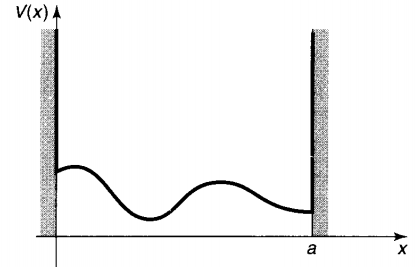
\includegraphics[width=0.4\textwidth]{figures/wkb1}
		\caption{The imagined potential in the bottom of an infinite well.}
		\label{fig:wkb1}
	\end{figure}
	
	I assume that $p(x)$ is real, the classical case, and thus $E>V(x)$ from equation \eqref{sch11}. From equation \eqref{sol} I find
	\begin{equation}
		\psi(x)\simeq\frac{1}{\sqrt{p(x)}}(C_+e^{i\phi(x)}+C_-e^{-i\phi(x)}),
		\label{sol4}
	\end{equation} 
	where
	\begin{equation}
		\phi(x)=\frac{1}{\hbar}\int_{0}^{x} p(x')dx'.
	\end{equation} 
	Using that $e^{\pm i x}=cos(x)\pm isin(x)$ I rewrite equation \eqref{sol4}
	\begin{equation}
		\psi(x)\simeq\frac{1}{\sqrt{p(x)}}((C_++C_-)cos(\phi(x))+(C_+-C_-)sin(\phi(x)).
		\label{sol5}
	\end{equation} 
	Since $\psi(x)\Rightarrow0$ at $x=0$ $C_++C_-=0$. Likewise, $\psi(x)\Rightarrow0$ at $x=a$, which results in $\phi(x)=n\pi$. Thus
	\begin{equation}
		\psi(x)\simeq\frac{1}{\sqrt{p(x)}}(C_+-C_-)sin(\phi(x)),
		\label{sol6}
	\end{equation} 
	where
	\begin{equation}
		\int_{0}^{a}p(x)dx=n\pi\hbar.
	\end{equation} 
	The quantization determines the approximate energy eigenvalues. They are determined by evaluating $p=\sqrt{2M(E-V(x))}$ and $\int_{0}^{a}p(x)dx=n\pi\hbar$ for $p(x)$ and equating the results. With $\phi(x)$ evaluated wave-function in equation \eqref{sol6} is also determined.
\end{example}

\begin{example}
	In this example I consider quantum tunneling, which corresponds to the non-classical case where $E<V$ and thereby $p(x)$ is imaginary. By setting $E<V$ I find from equation \eqref{sol}
	\begin{equation}
		\psi(x)\simeq\frac{C}{\sqrt{|p(x)|}}e^{\pm\frac{1}{\hbar}\int |p(x)|dx}.
		\label{sol7}
	\end{equation} 
	Quantum tunneling is non-classical because a particle of lower energy travels through a larger potential barrier. The probability of traveling through the barrier can be found by considering the wave function hitting the(a rectangular) barrier. I consider the scenario shown in figure \ref{fig:wkb2}.
	\begin{figure}[H]
		\captionsetup{width=1\textwidth}
		\centering
		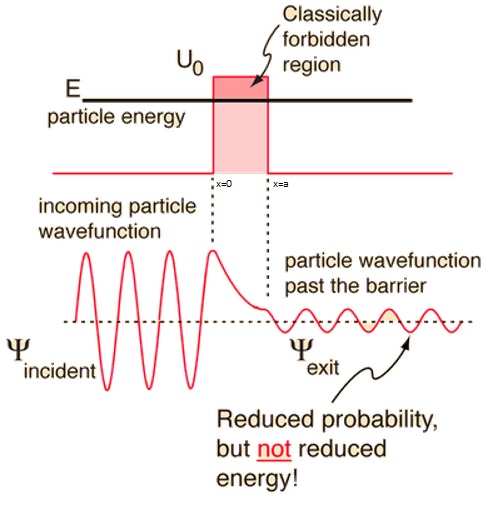
\includegraphics[width=0.5\textwidth]{figures/wkb2}
		\caption{Quantum tunneling.}
		\label{fig:wkb2}
	\end{figure}
	Analog to classical wave-physics, the involved waves will be an incident wave (I) a reflected wave(R) and a transmitted wave(T). I define $x=0$ where the wall starts, and $x=a$ where it ends. At $x<0$ the the incident and reflected wave is described by the wave function\footnote{The potential is constant, so the integral just evaluates to $x$.}
	\begin{equation}
		\psi_{x<0}(x)=Ie^{ik_1x}+Re^{-ik_1x},
	\end{equation} 
	where the subscript "$x<0$" denotes that this is the wave function for $x<0$, $I$ and $R$ are the amplitudes of the incident and reflected wave, respectively, and\footnote{At $x<0$ $V(x)=0$. I have used this in $p=\sqrt{2M(E-V(x))}$  along with $k=\frac{p}{\hbar}$.} $k_1=\frac{\sqrt{2ME}}{\hbar}$. I write the wave function in the tunneling region, $0<x<a$, as (with constant potential, $E_0$)
	\begin{equation}
		\psi_{0<x<a}(x)=C_1e^{ik_2x}+C_2e^{-ik_2x},
	\end{equation} 
	where $k_2=\frac{\sqrt{2M(E_0-E)}}{\hbar}$. I write the transmitted wave at $x>a$ as
	\begin{equation}
		\psi_{x>a}(x)=Te^{ik_1x}.
	\end{equation} 
	From my definitions the transmission probability is given by
	\begin{equation}
		P_{trans}=\frac{|T|^2}{|I|^2}.
	\end{equation} 
	I find $P_{trans}$ by evaluating the amplitudes $T$ and $I$ via imposing boundary conditions. I require continuity at the boundaries
	\begin{equation}
		\psi_{x<0}(0)=\psi_{0<x<a}(0),
	\end{equation} 
	\begin{equation}
		\frac{\partial \psi_{x<0}(0)}{\partial x}=\frac{\partial \psi_{0<x<a}(0)}{\partial x},
	\end{equation} 
	\begin{equation}
		\psi_{0<x<a}(a)=\psi_{x>0}(a),
	\end{equation} 
	\begin{equation}
		\frac{\partial \psi_{0<x<a}(a)}{\partial x}=\frac{\partial \psi_{x>0}(a)}{\partial x}.
	\end{equation} 
	From the BC I find
	\begin{equation}
		R=\frac{1}{2}\bigg(C_2(1-\frac{ik_2}{k_1})+C_1(1+\frac{ik_2}{k_1})\bigg),
	\end{equation} 
	\begin{equation}
		I=\frac{1}{2}\bigg(C_2(1+\frac{ik_2}{k_1})+C_1(1-\frac{ik_2}{k_1})\bigg),
	\end{equation} 
	\begin{equation}
		C_2=\frac{B_3}{2}(1-\frac{ik_1}{k_2})e^{-(ik_1+k_2)a},
	\end{equation} 
	\begin{equation}
		C_1=\frac{B_3}{2}(1+\frac{ik_1}{k_2})e^{(k_2-ik_1)a}.
	\end{equation} 
	Thus, I find the transmission probability ($P_{trans}$) as~\citep[p.340]{BR}
	\begin{equation}
		P_{trans}=\bigg|\frac{2k_1k_2e^{-k_1a}}{2k_1k_2cosh(k_2a)-i(k_1^2-k_2^2)sinh(k_2a)}\bigg|^2.
		\label{ptrans}
	\end{equation} 
	For large $k_2a$, which corresponds to small penetrations, I can make the small angle approximations
	\begin{equation}
		sinh(k_2a)\approx
		cosh(k_2a)\approx\frac{e^{k_2a}}{2}.
	\end{equation} 
	Thus, equation \eqref{ptrans} reduces to
	\begin{equation}
		P_{trans}\approx\bigg(\frac{4k_1k_2}{k_1^2+k_2^2}\bigg)^2e^{-2k_2a}.
		\label{ptrans2}
	\end{equation} 
	The first factor is down to reflection losses at the two boundaries ($x=0$ and $x=a$). The exponential describes the exponential decay of the amplitude of the wave function inside the barrier. The first factor varies slowly with energy and is therefore often neglected. Thus, the transmission probability is written as
	\begin{equation}
		P_{trans}\approx e^{-2k_2a}.
		\label{ptrans3}
	\end{equation} 
	Taking into account that the potential could be non-constant in the tunneling region, I find
	\begin{equation}
		P_{trans}\approx e^{-\frac{2}{\hbar}\int_{0}^{a}|p(x)|dx}=e^{-\frac{2}{\hbar}\int_{0}^{a}|\sqrt{2M(V(x)-E)}|dx},
		\label{ptrans4}
	\end{equation} 
	where $V(x)$ and $E$ has switched places because of the imaginary unit is "pulled out" and I consider the magnitude. From equation \eqref{ptrans4} it is clear that the incoming wave decays approximately exponentially inside the barrier, so the relationship between the incident and outgoing wave is the exponential decay. This squared gives the (approximate) transmission probability. The transmission probability is often used eg. in $\alpha$ particle decay or in nuclear fusion.
\end{example}